\documentclass[12pt,pdftex]{article}
\usepackage[pdftex]{graphicx,color}
\usepackage{setspace,palatino,multirow}
\usepackage{amsmath,amssymb}
\usepackage{titlesec}
\usepackage{lscape}
%\usepackage{subfigure}
\usepackage{threeparttable}
\usepackage{natbib}
\bibliographystyle{ecta}
\usepackage{cite}
\usepackage{booktabs}
\usepackage{subcaption}
\usepackage{pdflscape}
\usepackage{afterpage}
\usepackage{xcolor}
\usepackage{rotating}

\definecolor{nblue}{RGB}{0,0,128}

\usepackage[pdftex,colorlinks=true, bookmarks=false,
pdfstartview={XYZ null null 0.65},
pdftitle={Heterogeneous Agent Trade},
pdfauthor={ Michael E. Waugh},
pdfkeywords={economics, trade, dynamics, quant econ, consumption, data science,
waugh, incomplete markets, inequality, julia, Armington, Minneapolis Fed, price elasticity, distance, python, matplotlib},
colorlinks=true,linkcolor=darkgray,citecolor=darkgray,urlcolor=darkgray,
breaklinks]{hyperref}

\newcounter{saveeqni}%
\newcounter{saveeqn01i}%
\newcommand{\alpheqni}{\setcounter{saveeqni}{\value{section}}%
%\setcounter{saveeqn01i}{\value{subsectioni}}%
\renewcommand{\theequation}
    {\alph{saveeqni}\mbox{.\arabic{equation}}}}%
\newcommand{\reseteqni}{\setcounter{equation}{\value{saveeqni}}%
\renewcommand{\theequation}{\arabic{equation}}}%

\newtheorem{as}{Assumption}
\newtheorem{reg}{Regularity Condition}
\newtheorem{conjecture}{Conjecture}
\newtheorem{corr}{Corollary}
\newtheorem{df}{Definition}
\newtheorem{lemma}{Lemma}
\newtheorem{prp}{Proposition}
\newtheorem{rmk}{Remark}
\newenvironment{prf}{{\bf Proof}}{\hfill { }}

\DeclareMathOperator*{\plim}{plim}
\DeclareMathOperator*{\umax}{max}

\special{papersize=8.5in,11in}
\onehalfspacing
\setlength{\parindent}{0.1em}
\setlength{\parskip}{.09in}
\textwidth15.75cm
\evensidemargin 1.5in
\oddsidemargin 1.5in
\topmargin 8.5cm
\textheight 10in
\hyphenation{over-lapping}

\titleformat{\section}{\color{black}\large\bf}{\color{black}{\thesection.}}{.25cm}{}
\titleformat{\subsection}{\color{black}\normalsize\bf}{\thesubsection.}{.5em}{}
\titleformat{\subsubsection}{\color{black}\normalsize\bf}{\thesubsubsection.}{.5em}{}

\titlespacing{\section}{0pt}{*1.5}{*.5}
\titlespacing{\subsection}{0pt}{*1.5}{*.5}
\titlespacing{\subsubsection}{0pt}{*1.5}{*.5}

\def\thesection{\arabic{section}}
\def\thesubsection{\arabic{section}.\arabic{subsection}}
\def\thesubsubsection{\arabic{section}.\arabic{subsection}.\Alph{subsubsection}}

\def\citeapos#1{\citeauthor{#1}'s (\citeyear{#1})}

\renewcommand{\arraystretch}{1.1}
\usepackage[margin=2cm]{geometry}

\begin{document}

\begin{onehalfspacing}

{\large \textbf{\href{https://www.waugheconomics.com/uploads/2/2/5/6/22563786/heterogeneous-agent-trade.pdf}{Heterogeneous Agent Trade}}}

\vspace{0.5cm}

\href{http://www.waugheconomics.com/}{Michael E. Waugh} \\ Federal Reserve Bank of Minneapolis and NBER

\vspace{0.5cm}

\textbf{In Progress.} This draft: April 2023

\vspace{1.5cm}


\normalsize

ABSTRACT ------------------------------------------------------------------------------------------------------------

This paper develops a model of heterogenous agents and international trade. Heterogenous agents are modeled as in the standard incomplete markets tradition with households facing incomplete insurance against idiosyncratic productivity and taste shocks. Trade in goods follows the Armington tradition but is derived from the ``bottom up'' with micro-level heterogeneity shaping aggregate trade. I show how micro-level trade elasticities, trade, and the gains from trade vary with a household's wealth and how self-insurance motives shape these outcomes. In aggregate, the pattern of trade is distorted relative to the efficient allocation and the gains from trade deviate from standard benchmarks. Quantitatively, I compute the multi-country, asymmetric global economy and calibrate it to match bilateral trade flows for 19 countries. I use the model to measure the gains from trade and the first-best pattern of trade.

------------------------------------------------------------------------------------------------------------------------------
%%\vspace{0.25cm}
%
%%JEL Classification:
%%
%%
%%Keywords:

\vspace{6.0cm}

\footnotesize Email: michael.e.waugh@gmail.com. The views expressed herein are those of the author and not necessarily those of the Federal Reserve Bank of Minneapolis or the Federal Reserve System. This project was developed with research support from the National Science Foundation (NSF Award number 1948800). Thomas Hasenzagl provided excellent research assistance. My github repository provides the code and supplementary work behind this paper at \url{https://github.com/mwaugh0328/heterogeneous-agent-trade}.

\hspace{-0.05cm}



\thispagestyle{empty}
\newpage
\normalsize

This paper develops a model of heterogenous households and international trade. From the perspective of trade, household heterogeneity is interesting because of the notion that some benefit from trade and others don't. One aspect of these unequal gains relates to the idea that rich and poor consumers have different sensitivities to price and, thus, they shape the expenditure patterns and the gains from trade at the micro and macro level. I develop this idea in a model where heterogeneity in price sensitivity arises because of a market failure, i.e., the lack of insurance against life's circumstances. I then study the model's implications for aggregate trade, the gains from trade and how they are distributed, and the normative implications, e.g., what \emph{should} the pattern of trade look like.


An appealing feature of the model that I develop is that the ingredients are well known and workhorse frameworks within their respective literatures. Household heterogeneity is induced via the standard incomplete markets model (\citet{bewley1979optimum}, \citet{huggett1993risk}, \citet{aiyagari1994uninsured}) with households facing incomplete insurance against idiosyncratic productivity and taste shocks. Trade in goods follows the Armington tradition with producers in each country producing a national variety. The twist is that households have random utility over these varieties and they make a discrete choice over the varieties to consume (\citet{mcfadden1974frontiers}) in addition to their savings decisions. The explicit aggregation of household-level decisions then determines aggregate trade flows, trade elasticities, and the gains from trade.

The key force through which heterogeneity matters are trade (price) elasticities that vary with income and wealth at the household-level. I characterize household-level trade elasticities, their connection with savings motives, and how household-level elasticities translate to aggregates. Behind the math is the intuitive idea that poor households strongly value extra consumption|independent of the variety|as their marginal utility of consumption is high. So, poor households are very sensitive to price on both the intensive and extensive margin and then concentrate their expenditure on the cheapest commodity available. In contrast, rich households' marginal utility is low, are less sensitive to changes in prices, and likely consume their ideal variety independent of price. In aggregate, the pattern of trade and the response of trade to shocks|the aggregate trade elasticity|depends upon the micro-level trade elasticities and the distribution of demand.

The issues behind heterogeneity in price sensitivity lead to new perspectives on the welfare gains from trade. First, I show how one aspect of the household level gains from trade reflect the expected, discounted stream of changes in an individual's ``home choice probability,''  similar in spirit to the result of \citet*{arkolakis2012new}.

A second force is how a liberalization changes a household's valuation of its net asset position. The issue is that a trade liberalization will change interest rates and lead to winners and losers depending upon a households' net asset position. For example, if a trade liberalization leads to an increase in interest rates, net debtors suffer since their terms to borrow deteriorated, while net savers benefit. Why might a trade liberalization change interest rates? It's because of heterogenous effects on expenditure patterns and savings. For example, if the liberalization disproportionately benefits the rich /savers in the economy, they shed assets to consume a bit more and interest rates must increase to clear financial markets impacting the poor / debtors in the economy. The novelty here is how heterogeneity on the trade side links up with the financial market|not separate as they are typically treated or would occur in the knife-edge case discussed below.

%A third force is that there are true reallocation effects on the household side and these influence the aggregate gains from trade. As alluded to above, trade influences the households' incentives to consume and save, and, thus, where households ultimately reside in the distribution of wealth. So does a liberalization make it more or less likely that households are in ``good'' or ``bad'' parts of the distribution. As discussed below, this force is unique to the decentralized allocation and symptomatic of an inefficiency in the initial allocation.


Before moving on to the quantitative work, I explore two special cases. The first case is the efficient allocation where a planner can reallocate resources and overcome market incompleteness. In this case, I recover ``first-best intuition'' in that the gains from trade only reflect the direct savings associated with a reduction in trade costs. In this allocation, changes in expenditure patterns are not relevant via an envelope theorem argument|the planner already sources goods from the correct places so there are no gains from expenditure switching. While my economy is about heterogeneity on the household side, this result is reminiscent of \citet{AtkesonBurstein2010} and the irrelevance of firm heterogeneity in an economy where the allocation is efficient. Thus, the core issues at play in my model are not household heterogeneity per se, but inefficiencies induced by market incompleteness.

The second special case that I consider is when the utility function over the physical commodity is $\log$. With $\log$ utility, I obtain a separation result where aggregate trade outcomes ``separate'' from household heterogeneity. Trade takes a constant elasticity form with the trade elasticity pinned down by the dispersion parameter on the taste shocks similar to \citet{eaton2002technology}. And the trade elasticity and the share of home purchases summarize the gains from trade like in \citet{arkolakis2012new}. This case is also interesting because \citet*{anderson1987ces} showed that in a static model with log utility and additive logit shocks, the economy behaves \emph{as if} there were a representative agent CES consumer. In my economy, my suspicion was that market incompleteness and intertermporal behavior would nullify \citeapos{anderson1987ces} result|it does not.

Quantitatively, I make a contribution by computing and calibrating the model at a scale typically reserved for static trade models. As a testing ground, I focus on the data set of \citet{eaton2002technology}. The 19 countries in this data set is about the right size to easily illustrate how a very rich model like this can work in a multi-country setting. Moreover, the \citet{eaton2002technology} data set provides a well defined benchmark disciplined by bilateral trade flows and gravity variables|so it's a nice laboratory to explore new issues in.

The calibration challenge is the following. The model does not admit a ``gravity'' representation that allows researchers to invert trade frictions and productivity levels from trade flows as done, e.g., in \citet{eaton2002technology} and many subsequent papers. Similarly, the model does not admit the use of ``exact-hat algebra'' which allows the research to construct counterfactuals without the knowledge of primitives like trade frictions or productivity (see, e.g., the approach articulated in \citet{costinot2014trade} or the dynamic extension in \citet*{caliendo2015trade}).

My solution is to use the insight that the regressions employed in gravity frameworks provide very accurate descriptions of the data generating process. Rather than treating the gravity regression as a structural relationship, I use it as a ``guide'' and use an indirect inference procedure where I estimate parameters of the model so that the regression coefficients from a standard gravity regression run on my model's data match that seen in the data. This procedure works well and, thus, the model is able to match spatial distribution of economic activity in the data|just as well as standard, constant elasticity gravity models.

An outcome of the calibration is that trade elasticities decrease with the competitiveness of a source country in a destination. In other words, expensive products are more elastic relative to cheaper products. Behind this is what some might call a super-elasticity of trade within the model \emph{endogenously} delivering the result that elasticities increases with price and a pattern conforming with ``Marshall's Second Law of Demand.''

The final part of the quantitative analysis explores how trade behaves in the efficient allocation relative to that seen in the baseline model (and data). I should emphasize that this is a novel exercise than typical executed in the trade literature. Unlike the industry standard, I'm \emph{not} changing spatial, technological relationships (trade costs) and looking at how trade changes. What I'm doing is completing markets with the planner facing the same technological restrictions as private market participants and then asking what happens.

Two interesting things happen. Generally, the planner reduces trade in relationships that were already small. These are trading relationships that have the feature of being a luxury in the sense that it's mostly rich people engage in them. So when the planner redistributes within the country, trade ``catering to the rich'' is reduced. In contrast, the planner increases trade within already competitive relationships. An example of this is US imports with Japan, where the planner increases trade by nearly 5 percentage points. So here, the planner is using trade to ``service the masses'' as it redistributes.


Motivating my work has been a sequence of papers focusing on measuring the heterogenous impacts of trade on the consumer side. \citet{fajgelbaum2016measuring}, \citet{carroll2020heterogeneous}, \citet{borusyak2021distributional}, \citet{jaccardtoronto} are recent examples that measure heterogeneity in import exposure.\footnote{Its important for the reader to distinguish the pattern of heterogeneity across sectors vs. within a sector (\citet{cravino2017distributional} makes this distinction very clear). The evidence suggests that the patterns work in different directions with poor households consuming more traded goods, but within traded goods the poor consume lower price varieties and less imported content. My model is of one sector and about expenditure and substitution within that sector.} \citet*{auer2022unequal} and \citet*{colicev2022impact} go a step further measuring heterogeneity in price sensitivity across the income distribution and this type of evidence is very much the launching point for my paper.

While this work motivates my paper, I take a conceptually different approach. Rather than focusing on measurement, I take a model of household heterogeneity in price elasticities and study its implications. In this sense, my papers approach is most similar to \citet{fajgelbaum2011income} who study how heterogeneity in income and non-homotheticities (arising from a similar preference structure as mine) shape trade in vertically differentiated products.

A key feature of my work is that I start with a theory behind the distribution of income and wealth. This theory plus a demand system with heterogenous price elasticities then breaks aggregation in the goods market. And because aggregation is broken, it opens the door to new insights about trade, the interaction of trade and financial markets, and how market incompleteness shapes the aggregate pattern of trade.

% Connect with close economy stuff...evidence on prices


%because  within their respective literatures.
%
%
%
%
%%\footnote{Separate from this is computational challenge. Finding an equilibrium requires (i) solving for households dynamic problems|in each country (ii) constructing the stationary distribution of expenditure patterns and wealth|in each country (iii) aggregating and then (iv) finding a vector of prices so goods markets and financial markets clear world wide. Plot twist: It's doable. My github repository and the Appendix provides a complete description of my approach and methods.}
%
%
%then allows me to think explicitly about normative issues
%
%
%As a I show, market incompleteness is not a sufficient condition to




%Lit review:
%\begin{itemize}
%  \item FK paper, about heterogeneity in shares. This is about elasticities. They say model is pro-poor, but the issue is about sector. This is a model of within catagory/sector. Relates to Cravino Levchncho.
%
% \item Cravino Levchenko is about have a within discussion, they just don't see shares. But what they do see (in the is that high income guys buy high priced stuff). Then when constructing the price index, they assume this in some way. Simmilar to Krill. Key is to distingusih, income on price within varity, vs. income and shares (imported or not) and where they come from.

%  \item Note my formulas have similar flavor to fixed share approach. Planner is share times change is welfare gain. Need to look at krill paper.
%
%\item Krill paper... they do find that within category, rich buy more imported stuff than poor. The issue is complicated as you go across categories and then you do not get much action. The KN data set goes a deep dive and finds this as well. China is strange, strong case for thinking about qualit see Page 18 second to last paragraph. There you see the Armington quirk, imported stuff is more expensive, and rich guys are buying imported stuff. Other thing about Krill paper is critique of FK paper...AIDS generates a mechanical pro-poor bias. Non-homothetic CES is flexible to generate pattern in the data, FK is not. Final point, the Krill paper derives the share approach, this turns out to be exactly the same as the gains from trade in planner allocation
%
%\item Torston Jaccard does something simmilar to Krill, Auer. China messe stuff up, Europe strong pro rich exposure. All personal beuty products. Simmilar stuff to Auer. Proably more relavent for work with Simon is the stuff abour urban vs. rural and how this is above and beyond income, suggests something up about retailer. Does nested logit.
%
%\item The hotman paper is strange. This is mostly across sectors and claim they find something like Krill. No elasticity effect. Second, the Layspayers gives a totally different estimate than the model (inflation is high for poor vs rich) Why? Not really told that. The inflation results are suggestive that rich benefited more...but not quite obvious. Also not sure what the role of the firm is.
%
%\item Walsh paper...looks similar to my welfare calculations. Builds on the Moll paper too. Interesting is how they compute money metric by computing change in welfare relative to change in muc. Should put in labor income channel.
%
%\item Moll paper is very slick. Again more related than Walsh. One thing they do is put things in a money metric units by dividing through by muc in period 0. In the efficient economy, this then is back to Krill's formula. This money metric formula is why things are discounted by $R$ in Walsh...because the euler equation implies the ratio of muc's are equal to $R$. The other trick about this is that when assets are in zero net supply, the aggregate welfare gain in money metric units is zero. Key is that it's in money metric units though, in utils space there is true redistribution (worth talking about in either finacial globalization space or finacial autarky world).
%
%\item Is kind of related to Auclart...this the interest rate exposure channel. Less than I thought. As the key thing is more about dc. Tobin quote is nice about heterogenaity in muc. Everything is short term assets, so like in the moll paper sales = stocks. And then some people have different unhedge exposures to changes in interest rates.
%\end{itemize}


%This pattern of elasticities is consistent with recent evidence focusing on expenditure switching at the household level. \citet*{auer2022unequal} explore the heterogenous impact of the 2015 Swiss Franc appreciation and find that the exchange rate shock lead to larger changes in expenditure shares for poor households relative to the rich. In other words, poor households are more sensitive to price than rich households. Outside of the trade literature, there is broader set of evidence in support of the idea that price sensitivity declines with income; e.g. \citet{sangani2022markups} provides evidence in support of this fact using Nielsen Homescan data.
%%Discuss this evidence better. Faber Falley, Dellevingo,


\section{The Heterogeneous Agent Trade Model}

This section describes the model and then defines the decentralized competitive equilibrium. Trade is in the Armigton tradition with each country producing a nationally differentiated variety. Households face the ``income fluctuations problem'' as in the standard incomplete markets tradition (see, e.g., Chapter 17 of \citet{ljungqvist2012recursive}).

The key twist is that I do not employ modeling techniques with aggregation at household level across national varieties. Instead, I lean into the household heterogeneity and have households make a discrete choice over the varieties they consume in addition to their savings decisions. Aggregate trade flows, trade elasticities, and the gains from trade are then defined by the explicit aggregation of household-level decisions to purchase different varieties, their elasticity of demand, and their gains from trade.

\subsection{Production and Trade}\label{sec:trade}

There are $M$ locations which I call a country. Each country produces a nationally differentiated product. In country $i$, competitive firms' production technology to produce variety $i$ is:
\begin{align}
Q_i = A_i N_i,
\label{eq:production}
\end{align}
where $A_i$ is total factor productivity and $N_i$ are the efficiency units of labor supplied by households in country $i$.\footnote{Note that lack of physical capital in the model. Households here are saving in via pure exchange of non-state contingent IOUs as in \citet{huggett1993risk} rather than in physical capital as in \citet{aiyagari1994uninsured}.}

In the next several sections, I focus on only one type of barrier to trade: there are iceberg trade costs $d_{ij} > 1$ for a good to go from supplier $j$ to buyer $i$.

Profit maximization of the producers in location $i$ results in the wage per efficiency unit reflecting the value of the marginal product of labor
\begin{align}
w_{i} = p_{i} A_{i}.
\label{eq:marginal-product}
\end{align}
Given iceberg trade costs, the unit cost for country $i$ to purchase a good from location $j$ is
\begin{align}
p_{ij} = \frac{d_{ij}w_{j}}{A_{j}}.
\label{eq:marginal-product-ship}
\end{align}
This is the trade and production side of the model. While sparse, it's worth reminding you that with a representative agent and a constant elasticity Armigton aggregator much comes out of this model. There is a ``gravity equation'' relating bilateral trade flows to country characteristics with a constant trade elasticity. And there are two sufficient statistics (the trade elasticity and home trade share) that globally characterize the welfare gains from trade. In the next section, I give up on the representative agent.

\subsection{Households}

There is a mass of $L_i$ households in each country. Households are immobile across countries. They are infinite lived and have time-sparable preferences over consumption of varieties:
\begin{align}
E_{0} \sum_{t = 0}^{\infty} \beta^{t} \tilde{u}( \{ c_{ijt} \}_{M}),
\end{align}
where the notation $\{ c_{ijt} \}_{M}$ means that the household has preferences over all $j$ varieties supplied by $M$ countries in the world. Here I'm indexing things by $ij$ to denote the variety $j$ that is consumed in location $i$.

Households' period utility function is of the random utility class and each period households can only consume one variety. The utility associated with the choice of variety $j$ is
\begin{align}
\tilde{u}( c_{ijt} ) =  u(c_{i,t}) + \epsilon_{jt}. \label{eq:utility}
\end{align}
where the $\epsilon_{jt}$ are iid random variables across time, households, and countries. For the analysis, I assume that these shocks are distributed Type 1 Extreme Value with CDF
\begin{align}
F(\epsilon) &= \exp(-\exp(-\sigma_{\epsilon}^{-1}\epsilon))
\end{align}
where $\sigma_{\epsilon}$ is the dispersion parameter. A useful generalization of this setting to a multi-sector model is the ``infinite shopping isle'' approach of \citet{p-iq} where these shocks take on a Generalized Extreme Value representation and then households choose the sector and then the variety each period.

For now, all I assume that the utility function over the physical good $c_{ijt}$ is well behaved. In the analysis below I explore different specifications of the utility function $u$ over the physical commodity and I highlight the rather unique case of $\log$ utility.

A household's efficiency units are stochastic and they evolve according to a Markov chain. So, $z$ is a household's efficiently units and $\mathcal{P}(z,z')$ describes the probability of a household with state $z$ efficiency units transiting to state $z'$. Again, I assume that $\mathcal{P}$ is well behaved in the necessary ways.

Households can save and borrow in a non-state contingent asset $a$. One unit of the asset pays out with gross interest rate $R_i$ next period. I discuss this more in depth below, but the determination of $R_{i}$ is with that which clears the bond market (local or global). A country specific, exogenous debt limit $\phi_{i}$ constrains borrowing so:
\begin{align}
a_{t+1} \geq - \phi_{i}.
\label{eq:borrowing-constraint}
\end{align}
All these pieces come together in the household's budget constraint, conditional on choosing variety $j$ to consume, and focusing on a stationary setting where prices are constant:
\begin{align}
p_{ij}c_{ijt} +  a_{t+1} \leq    R_{i} a_{t} + w_{i} z_{t}.\label{eq:trade-budget-constraint}
\end{align}
The value of asset purchases and consumption expenditures must be less than or equal to asset payments and labor earnings.

\subsection{The Household Problem}

The state variables of a individual household are its asset holdings and efficiency units. As alluded to above, for now I focus on a stationary setting where aggregates are not changing and, thus, I abstract from carrying the notation associated with them around.\footnote{If you \emph{do} want to carry them around, notice that all that households in each country care about are prices (today and in the future). The distributions of households in other countries, per se, don't matter. Thus, the relevant aggregate states in country $i$ are $\big [ \ \{ w_i \}_{M}, R_i \big ]$ which is the collection wage per efficiency units and the interest rate.}

The value function of a household in country $i$, after the variety shocks are realized, is
\begin{align}
v_{i}(a, z) = &  \max_{j} \big  \{ \  v_{i}(a, z, j)  \ \big \}
\label{eq:valuefun}
\end{align}
which is the maximum across the value functions associated with the discrete choices of different national varieties. The value function conditional on a choice of variety is
\begin{align}
v_{i}(a, z, j) = &  \max_{\ a' \ }\bigg  \{ u(c_{ij}) + \epsilon_{j}  + \beta \, \mathbb{E} [v_{i}(a', z')]  \bigg\}
\label{eq:value_fun_option} \\
\nonumber \\
\mbox{subject to}  \ & (\ref{eq:borrowing-constraint}) \  \mathrm{and} \ (\ref{eq:trade-budget-constraint}) \nonumber
\end{align}
where households choose asset holdings and the level of consumption is residually determined through the budget constraint. Associated with the solution to this problem is a policy function $g_{i}(a,z, j)$ which solves (\ref{eq:value_fun_option}) and maps current states into asset holdings tomorrow $a'$ contingent upon the variety choice $j$. The continuation value function on the right-hand side of (\ref{eq:value_fun_option}) is the expectation over (\ref{eq:valuefun}) with respect to (i) efficiency units next period, $z'$ and (ii) the variety taste shocks. An implication of this is that households understand that their may be situations where they really desire, say, a high priced imported good and, hence, save accordingly.

The Type 1 extreme value distribution on the taste shocks give rise to the following choice probabilities for each differentiated good:
\begin{align}
\pi_{ij}(a, z) = \exp \left( \frac{ v_{i}(a, z, j) }{\sigma_{\epsilon}} \right) \Bigg / \sum_{j'} \exp \left( \frac{ v_{i}(a, z, j') }{\sigma_{\epsilon}} \right), \label{eq:choice-prob}
\end{align}
which is the probability that a household with assets $a$ and efficiency units $z$ chooses country variety $j$. And then the expectation of (\ref{eq:valuefun}) with respect to the taste shocks takes the familiar log-sum form
\begin{align}
v_i(a, z) = \sigma_{\epsilon} \log \left\{ \sum_{j'} \exp \left( \frac{  v_{i}(a, z, j')}{\sigma_{\epsilon}} \right) \right\}. \label{eq:log_sum}
\end{align}
Associated with this problem in (\ref{eq:value_fun_option}) for non-borrowing-constrained households is a Euler Equation for each variety choice $j$:
\begin{align}
\frac{u'(c_{i}(a, z, j))}{p_{ij}} = \beta R_{i} \mathrm{E}_{z'} \left[ \sum_{j'} \pi_{ij'}(a', z') \frac{u'(c_{i}(a', z', j'))}{p_{ij'}} \right].
\label{eq:euler_equation}
\end{align}
This has a very natural interpretation: a household equates marginal utility of consumption today with expected discounted marginal utility of consumption tomorrow adjusted by the return on delaying consumption. The interesting feature here is that the expected value of the marginal utility of consumption reflects the uncertainty over one's preference over different varieties tomorrow via the choice probabilities. And note that households has some control over these probabilities as the asset choice today influence the choice probabilities tomorrow.

Before moving on to aggregation, I make one useful observation that assists the analysis. Stare at (\ref{eq:choice-prob}) and (\ref{eq:log_sum}) long enough, one can arrive at a dynamic, sufficient statistic representation of $v_i(a, z)$. Appendix \ref{apx-sec:gains-trade} works through the individual steps, but (\ref{eq:log_sum}) can be summarized as
\begin{align}
v_i(a, z) = -\sigma_{\epsilon} \log \pi_{ii}(a,z) + u(c_{i}(a,z,i)) + \beta \mathbb{E}_{z'} v_{i}(a',z').
\label{eq:log_sum-home}
\end{align}
Here the ex-ante value function (prior to the realization of the preference shocks) is expressed as a sum of the log home choice probability, utility over physical consumption of the home good, and recursively the expected value function tomorrow. What's going on here is that the home choice probability $\pi_{ii}$ summarizes the expected value of the taste shocks, their benefits, and how households respond to them in the future.\footnote{Home choice probabilities are not necessarily the same as home trade shares, but this is closely related to Equation (15), Footnote 42 of \citet{eaton2002technology} and I'm heading towards situations where this result plus restrictions on $u$ give rise to the result in \citet{arkolakis2012new}.}

Equation (\ref{eq:log_sum-home}) together with (\ref{eq:euler_equation}) also provides more insight about how households' savings motives interact with the variety choice. Focusing on a household consuming the home good (and note that the left-hand-side below could be for any variety choice), the Euler Equation in (\ref{eq:euler_equation}) becomes:
\begin{align}
\frac{u'(c_{i}(a,z,i))}{p_{ii}} = \beta \mathrm{E}_{z'} \bigg \{ -\sigma_{\epsilon} \frac{\partial \pi_{ii}(a',z') / \pi_{ii}(a',z')}{\partial a'} + \frac{u'(c_{i}(a',z',i))R_i}{p_{ii}} \bigg \},
\label{eq:euler_equation-home}
\end{align}
which says that an unconstrained household should be indifferent between the marginal utility of consumption forgone to hold some more assets and two components: (i) the benefit from how a change in assets changes in their variety choice in the future and this is summarized by the change in the home choice probability and (ii) the direct benefit of the returns on the assets evaluated at the marginal utility of consumption.

\subsection{Aggregation}

\textbf{Aggregation.} At the core of aggregation is a probability distribution $\lambda_{i}(a, z)$ describing the measure of households across the individual states. This distribution evolves according to
\begin{align}
\lambda_i(a', z') = \sum_{j} \int_{z}\int\displaylimits_{a: a' = g_{i}(a, z, j)} \pi_{ij}(a, z) \mathcal{P}(z, z') \lambda_i(a, z) \ da \ dz.
\label{eq:law_motion}
\end{align}
where the inner most term describes the mass of households choosing variety $j$, multiplied by the probability that $z$ transits to $z'$, multiplied by the existing measure of households with states $a$ and $z$. This is integrated with respect to those actually choosing asset holdings $a'$, over all $z$'s, and then summed over the different variety choices.

Given this distribution, everything else follows. First focusing on trade, aggregate bilateral imports are
\begin{align}
M_{ij} = L_i \int_{z} \int_{a}  p_{ij} c_{i}(a, z, j) \pi_{ij}(a, z) \lambda_i(a, z) \ da \ dz.
\label{eq:imports}
\end{align}
Here imports take on a mixed logit formulation that very much mimics that used in the industrial organization literature, e.g, \citet*{berry1995automobile}.

There are, however, several interesting differences in that there is an active intensive margin (not unit demand) and inside the choice probability $\pi_{ij}(a, z)$ is the non-linear value function from (\ref{eq:valuefun}). These features are interesting because they're determined by the dynamic features of the household problem. The household's inter-temporal choice to save determines the quantity choice. And because the choice probability reflects the value function, it embeds forward looking behavior of the household.

The third interesting feature is that the mixing distribution|over which demands are aggregated|is endogenous. Through the law of motion in (\ref{eq:law_motion}) household behavior determines the distribution of wealth. So it's not a free parameter and it will change with changes in primitives of the environment.

Similar to imports, aggregate bilateral exports from country $i$ to country $j$ are
\begin{align}
X_{ji} = L_j \int_{z} \int_{a}  p_{ji} c_{j}(a, z, i) \pi_{ji}(a, z) \lambda_i(a, z)da \ dz.
\label{eq:exports}
\end{align}
The value of aggregate consumption is
\begin{align}
\widetilde{P_{i} C_i}  &=  L_{i} \sum_{j} \int_{z} \int_{a}  p_{ij} c_{i}(a, z, j) \pi_{ij}(a, z) \lambda_i(a, z)da \ dz \label{eq:bigC}
\end{align}
In (\ref{eq:bigC}), one can see both a bug and a feature of this model. Here there is an ``index number problem`` in the sense that there is not an ideal price index for which one can decompose aggregate values in to a price and quantity component. This is in contrast to, e.g., a model where households consume a CES bundle of goods.

Finally, the aggregate quantity of asset holdings integrates across the asset choices of individual households
\begin{align}
\mathrm{A}_i' = L_{i}\sum_{j} \int_{z} \int_{a}  g_{i}(a, z, j) \pi_{ij}(a, z) \lambda_i(a, z) da \ dz.
\label{eq:aggregate_asset}
\end{align}
which integrates over the asset choices|given the policy function $g_{ij}(a, z)$ and variety choices $\pi_{ij}(a, z)$. And then sum's across the different varieties available.

\textbf{National Accounting.} From here, I reconstruct national income and product identities. Starting from the production side, aggregate efficiency units are
\begin{align}
N_i = L_{i}\int_{z} \int_{a}\ z \lambda_i(a, z) da \ dz. \label{eq:ag-labor-supply}
\end{align}
and from here we can connect the value of aggregate production must equal aggregate payments to labor so
\begin{align}
p_{i} Y_{i} = p_{i} A_{i} N_{i} = L_i \int_{z} \int_{a} w_{i} \ z \ \lambda_i(a, z) da \ dz,
\label{eq:value_production}
\end{align}
Then by summing over individual consumers' budget constraint and substituting in (\ref{eq:value_production}), the aggregated budget constraint is:
\begin{align}
p_{i} Y_{i}  = \widetilde{P_{i} C_i}  + \bigg[-R_i\mathrm{A_i} +  \mathrm{A_i'} \bigg],
\label{eq:aggregate_budget_constraint}
\end{align}
where national income equals the value of aggregate consumption $\widetilde{P_{i} C_i}$ and the country's net factor payments and net asset position. To arrive at the standard national income accounting identity, simply work with the relationship between production, exports, and aggregate consumption in (\ref{eq:bigC}) and imports gives rise to
\begin{align}
p_{i} Y_{i}  = \widetilde{P_{i} C_i} + \bigg[\ \sum_{j\neq i}X_{ji} -  \sum_{j\neq i}M_{ij} \bigg],
\label{eq:gdp}
\end{align}
where national production or GDP equals consumption plus exports minus imports. A comparison of (\ref{eq:aggregate_budget_constraint}) and (\ref{eq:gdp}) then makes clear that the trade imbalance is connected with a countries net factor payments and net asset position.

Beyond accounting, this last observation shows how trade flows are interlinked with financial flows. Inspection of the individual elements in (\ref{eq:imports}), (\ref{eq:aggregate_asset}), and the households' budget constraint reveal that household's asset positions are intertwined with trade flows through both the intensive (how much to consume and, hence, save) and the extensive margins (which variety to consume). Thus, a feature of this model is that the trade side is interlinked with the financial side of the economy in a non-trivial way.

\subsection{The Decentralized Equilibrium}

In this section, I discuss the market clearing conditions that an equilibrium must respect and then define the Decentralized Equilibrium of this economy.

\textbf{The Goods Market.} Goods market clearing equates the value of production of commodity $i$  with global demand for country $i$'s commodity:
\begin{align}
p_{i} Y_{i} &= \sum_{j}  X_{ji} \label{eq:goods-supply},
\end{align}
where the left hand side is production and the right hand side is world demand for the commodity (via exports) from (\ref{eq:exports}).

\textbf{The Bond Market.} The second market clearing condition is the bond market. There are two case worth thinking about here. One is of ``financial autarky'' in which there is a local bond market that facilitates within country asset trade, but not across countries. In this case, there is an interest rate $R_i$ for each country and the associated market clearing condition is
\begin{align}
\mathrm{A_i'} = 0, \ \ \forall i
\label{eq:bond-market-country}
\end{align}
which says that net asset demand within each country $i$ must be zero. As is common in the trade literature, this condition implies that trade is balanced|just stare at (\ref{eq:aggregate_budget_constraint}) and (\ref{eq:gdp}). Yet, even with balanced trade, there is still within country trade of financial assets. Some households are savers, others are borrowers and the interest rate is that which the net asset position is zero.

The second case is of ``financial globalization'' where there is a global bond market that facilitates both within country asset trade, and across countries. In this case, there is a single interest rate $R$ and the associated market clearing condition is
\begin{align}
\sum_{i}\mathrm{A_i'} = 0
\label{eq:bond-market-globalization}
\end{align}
In this case trade need not be balanced for each country. Here a specific country might run, say, a trade deficit because at the given prices, the total amount of borrowing within a country is larger than the total amount of saving. However, across all countries total borrowing must equal total saving.

Below I formally define the Decentralized Stationary Equilibrium where private market participants taking prices as given solve their problems, the distribution of households is stationary, and prices are consistent with market clearing.

\textbf{The Decentralized Stationary Equilibrium.} A Decentralized Stationary Equilibrium are asset policy functions and commodity choice probabilities $\{\  g_{i}(a, z, j), \pi_{ij}(a, z) \ \}_{i}$, probability distributions $\{ \ \lambda_i(a, z) \ \}_{i}$ and positive real numbers $\left \{w_i, p_{ij}, R_i\right \}_{i,j}$ such that
\begin{itemize}
\vspace{-.4cm}
\item[i]  Prices ($w_i, p_{ij}$) satisfy (\ref{eq:marginal-product}) and (\ref{eq:marginal-product-ship});
\item[ii] The policy functions and choice probabilities solve the household's optimization problem in (\ref{eq:valuefun}) and (\ref{eq:value_fun_option});
\item[iv] The probability distribution $\lambda_i(a, z)$ induced by the policy functions, choice probabilities, and primitives satisfies (\ref{eq:law_motion}) and is stationary;
\item[v] Goods market clears:
\begin{align}
p_{i} Y_{i} - \sum_{j}^{M}  X_{ji} = 0, \ \ \forall i
\end{align}
\item[v] Bond market clears with either
\begin{align}
\mathrm{A_i'} = 0, \ \ \forall i \ \ \ \mbox{or} \ \ \ \sum_{i}\mathrm{A_i'} = 0
\label{eq:fa-condition}
\end{align}
\end{itemize}

\subsection{Outline of the rest of paper}

This model above has households making individual choices over national varieties, savings, all while facing productivity and taste shocks. Explicit aggregation of household behavior determines the pattern of trade and this is linked with trade in financial assets.  The remaining sections of the paper work through the following questions:
\begin{enumerate}
\item \textbf{What does the efficient, centralized allocation look like?} The model features an inefficiency arising from market incompleteness. Households would like insurance against future shocks to income and taste shocks, but only have a partial ability to provide themselves this insurance. Endowing a central planner with the ability to overcome this friction and studying the resulting allocation helps illustrate the behavior of model in the decentralized allocation.

\item \textbf{What are the gains from trade in decentralized allocation?} Here, surprisingly, a lot can be said. I connect the results with those from the Centralized Allocation. I also workout a knife edge case when utility is $\log$ over consumption and how it delivers complete separation between the heterogenous agent side of the economy and trade.

\item \textbf{What are the quantitative implications of this model?} In this section, I calibrate the model essentially replicating the analysis of \citet{eaton2002technology} by selecting trade costs and productivity parameters so that bilateral trade flows in the model line up in the data. I then perform several counterfactuals to illustrate the mechanics of the model and make comparisons to the model of \citet{eaton2002technology} and the response of the centralized allocation.
\end{enumerate}

\section{The Centralized Allocation}\label{sec:planner}

This section describes the Centralized (Efficient) Allocation. The starting point is a stance on the social welfare function. I focus on a additive social welfare:
\begin{align}
W = \sum_{t=0}^{\infty} \sum_{i}  \int\limits_{z} \beta^{t} \psi_{i} v_{i}(z,t) L_{i}\lambda_{i}(z,t),
\nonumber
\end{align}
and here $v_i(z,t)$ is a households ex-ante utility (before preference shocks are realized) with state $z$, time $t$, in country $i$. The $\psi_{i}$ terms are country specific Pareto weights. And $\lambda_{i}(z,t)$ is the distribution of households in country $i$ across productivity states at date $t$. Now unpack the benefits from physical commodity and the preference shock in the following way:
\begin{align}
W = \sum_{t=0}^{\infty}  \sum_{i} \sum_{j} \int\limits_{z}  \beta^{t} \psi_{i} \  \bigg \{  u(c_{i}(z, j, t) ) + \mathrm{E}[ \ \epsilon \ | \ \pi_{ij}(z,t) ] \bigg \}\pi_{ij}(z,t) L_{i} \lambda_{i}(z, t)
\label{eq:social-welfare-2}
\end{align}
so the inner term is period utility given the associated consumption allocation and then the expected value of the preference shock conditional on the choice probability $\pi_{ij}(z,t)$. This inner term is then weighted by the number of households that receive that utility, i.e., the choice probability times the mass of households with shock $z$ at date $t$. The sum across $j$ adds up all households in country $i$. Then the sum across $i$ reflects that this is global welfare.

The Planner chooses consumption allocations $c_{i}(z, j, t)$ and choice probabilities $\pi_{ij}(z,t)$ for all $i,j$ pairs, $z$ states, and dates $t$ to maximize (\ref{eq:social-welfare-2}). This maximization problem is subject to two constraints. The first is the resource constraint:
\begin{align}
Y_{it} \  \geq \ \sum_{j} \int_{z} d_{ji} c_{j}(z, i, t) \pi_{ji}(z,t) L_{j}\lambda_{j}(z, t),
\label{eq:planner_rc}
\end{align}
which says that production of variety $i$ must be greater than or equal to world consumption of variety $i$ inclusive of trade costs $d_{ji}$. The second constraint is that the choice probabilities are probabilities and sum to one:
\begin{align}
1 = \sum_{j}\pi_{ij}(z,t).
\label{eq:planner_choice_probs}
\end{align}
Given these constraints I define the \textbf{Centralized Planner's Problem} as the following:
\begin{align}
&\max\limits_{c_{i}(z, j, t),\ \pi_{i,j}(z, t)} \ \sum_{t=0}^{\infty}  \sum_{i} \sum_{j} \beta^{t} \int\limits_{z}   \  \bigg \{  u(c_{i}(z, j, t) ) + \mathrm{E}[ \ \epsilon \ | \ \pi_{ij}(z,t) ] \bigg \}\pi_{ij}(z,t) L_{i} \lambda_{i}(z, t) \ \ \label{eq:planner_problem}\\
\nonumber \\
& \ \ \mbox{subject to} \ \ (\ref{eq:planner_rc}), \ (\ref{eq:planner_choice_probs}) \ \mbox{and an inital condition} \ \ \lambda_i(z, 0).
\end{align}
In Appendix \ref{sec:apx-planner}, I derive the solution to this problem. Proposition \ref{prp:efficient-allocation} describes the allocation that maximizes social welfare and I will call this allocation the Efficient Allocation.

\begin{prp}[\textbf{The Centralized (Efficient) Allocation}]\label{prp:efficient-allocation} The allocation that satisfies the Centralized Planning Problem in (\ref{eq:planner_problem}) is:
\begin{enumerate}
\item A consumption allocation satisfying:
\begin{align}
\psi_{i} u'(c_{i}(z,j,t) ) = \chi_{j}(t) d_{ij}
\label{eq:planner-consumption}
\end{align}
where $\chi_{j}(t)$ is the shadow price of variety $j$.
\item The choice probabilities are
\begin{align}
\pi_{ij}(t) =\exp \left( \frac{u(c_{i}(j, t)) - u'(c_{i}(j, t))c_{i}(j,t)}{\sigma_{\epsilon}}\right) \bigg / \sum_{j'}\exp \left( \frac{u(c_{i}(j',t)) - u'(c_{i}(j', t))c_{i}(j', t)}{\sigma_{\epsilon}} \right)
\label{eq:planner-choice-prob}
\end{align}
and are independent of $z$ because of (\ref{eq:planner-consumption}).
\end{enumerate}
\end{prp}
Proposition \ref{prp:efficient-allocation} has some neat features. First, the consumption allocation takes on the natural feature that the (Pareto-weighted) marginal utility of consumption equals its shadow price adjusted by the trade friction. Here the shadow price is the multiplier $\chi_{j}(t)$ on the resource constraint in (\ref{eq:planner_rc}). Because the shadow price only reflects the scarcity of the commodity, the marginal utility of consumption (and consumption) then does not depend upon the household's state $z$. So if a household is productive or unproductive at date, $t$, the Planner equates the marginal utility of consumption across these states|within variety. This is the sense in which the planner is providing full insurance across households.

Another implication of (\ref{eq:planner-consumption}) is that the marginal utility of consumption is \textit{not} equated across all households within a country as one would typically expect in a one good model. (\ref{eq:planner-consumption}) implies that the ratio of the marginal utility of consumption|adjusted by relative shadow prices|should be equal. This is like a within-country \citet{backus1993} condition.

The second part of Proposition \ref{prp:efficient-allocation} prescribes the mass of households that consume variety $j$. Per the distributional assumption on the taste shocks, the choice probabilities in (\ref{eq:planner-choice-prob}) take the form of ratio's of $\exp$ relative to sum of $\exp$ functions with the dispersion parameter $\sigma_{\epsilon}$ showing up in the natural way.

The interpretation of the terms within the $\exp$ function take on a very intuitive form: it's the net social benefit of assigning a household to consume that variety.\footnote{A precursor to this result are the migration probabilities derived in \citet*{lagakos2023welfare} in the planing problem for their economy.} Net is here because it's the difference between the utility received $u(c_{i}(j,t))$ minus the social cost $u'(c_{i}(j,t))c_{i}(j,t))$. Why is the social cost? From (\ref{eq:planner-consumption}), the marginal utility of consumption exactly reflects the scarcity of providing $c_{i}(j,t)$. Thus, the interpretation is that variety assignment is based upon the social benefit net of providing that benefit.

Given Proposition \ref{prp:efficient-allocation}, I can compute the welfare gains from a change in trade costs. I do this by focusing on stationary allocations, so $t$'s are not relevant. And then study how welfare changes across the two stationary allocations. Here it is of no consequence as there is no moving aggregate state variable in the allocation, so the jump across stationary equilibrium is instantaneous.

Appendix \ref{sec:apx-planner} works out the details, Proposition \ref{prp:gains-efficient-allocation} describes the result.

\begin{prp}[\textbf{Trade Elasticities and Welfare Gains in the Efficient Allocation}]\label{prp:gains-efficient-allocation} The elasticity of trade to a change in trade costs between $i,j$ in the efficient allocation is:
\begin{align}
\theta_{ij} =  -\frac{1}{\sigma_{\epsilon}} \bigg [ u'(c_{i}(j)) c_{i}(j) \bigg]. \label{eq:eff-trade-elasticity}
\end{align}
And the welfare gains from a reduction in trade costs between $i,j$ are
\begin{align}
\frac{\mathrm{d} W}{\mathrm{d} d_{ij} / d_{ij}} = \frac{\partial W}{\partial d_{ij} / d_{ij}} = \frac{1}{1-\beta} \times \psi_{i} \ u'(c_{i}(j)) c_{i}(j) \pi_{ij} L_i
\label{eq:eff-trade-gains}
\end{align}
which is the discounted, direct effect from relaxing the resource constraint in (\ref{eq:planner_rc}).
\end{prp}
Proposition \ref{prp:gains-efficient-allocation} highlights a couple of things. First, consistent with intuition from \citeapos{eaton2002technology} Ricardian model, the dispersion parameter matters inversely. So if $\sigma_{\epsilon}$ is small, national varieties are ``as if they are near substitutes'' and thus trade flows will respond a lot. What is relatively non-standard is that the marginal utility of consumption times consumption shows up here and makes this trade elasticity $i,j$ specific. This is a generic feature of the environment and I discuss this point more below.

The second part of Proposition \ref{prp:gains-efficient-allocation} says that the total change in welfare only reflects the direct effect from relaxing the resource constraint, then discounted for the infinite future, hence the $1/ (1-\beta)$ term. Behind this result is an envelope-type argument with direct effects only mattering because I'm evaluating the change in welfare at the optimized allocation and any benefits of adjusting consumption and choice probabilities are zero|on the margin.

What is the direct effect? It equals the amount being eaten $c_{i}(j) \pi_{ij}(t) L_i$ times the valuation of the commodity which is the marginal utility of consumption. In other words, the gains from trade come from the destruction of less resources by trade costs, this directly allows for more consumption, an it's converted to utils by the marginal utility of consumption.

This result is reminiscent of \citet{AtkesonBurstein2010} who make a similar claim in the context of a model with rich firm heterogeneity. More specifically, they argue that the only first order effect lower trade costs have on welfare is the direct consumption effect and that indirect effects are second order. This is similar, but with household heterogeneity, by saying that, in the efficient allocation, the welfare gains are these direct consumption benefits.

As mentioned above, the non-standard thing is that the trade elasticity is $i,j$ specific and reflects the marginal utility of consumption times consumption. When preferences are $\log$
\begin{align}
\theta_{ij} = -\frac{1}{\sigma_{\epsilon}} \ \ \ \forall \ \ i,\ j,
\end{align}
the trade elasticity is \textit{not} $i,j$ specific and it exactly mimics \citet{eaton2002technology}. And it connects with \citet{anderson1987ces} and \citet{anderson1992discrete} (who focus on the log preference case), in that trade here behaves as if there were a representative agent Armington-CES consumer. I discuss this case in the decentralized allocation more below in Section \ref{}

Proposition \ref{prp:gains-efficient-allocation} is useful because it sets a benchmark for thinking about the role that incomplete markets is playing. It also highlights an interesting observation, that outside of $\log$ preferences, the random utility model naturally introduces a form of non-homotheticity. And, even in the efficient allocation, this is shaping how aggregate trade is responding to changes in trade costs.


\section{Trade Elasticities and the Gains from Trade}

This section focuses on the decentralized equilibrium and works towards understanding outcomes like trade elasticities and gains from trade (as in Proposition \ref{prp:gains-efficient-allocation}). I show how micro-level decisions shape the aggregate trade elasticity and then the gains from trade and the sources of those gains.

\subsection{Trade Elasticities}\label{sec:trade-elasticity}

My definition of the trade elasticity is the partial equilibrium response of imports from $j$ relative to domestic consumption due to a permanent change in trade costs.\footnote{Because the aggregate distribution of households will adjust|even with prices fixed|the elasticities that I derive are in a sense ``short-run'' elasticities.} By partial equilibrium, I mean that wages, interest rates, and the distribution of agents are fixed at their initial equilibrium values. This is consistent with the definition of the trade elasticity in say, \citet{arkolakis2012new} or \citet{simonovska2014elasticity}. By permanent, I mean that the change in trade costs is for the indefinite future and that households correctly understand this.

Given this discussion, my mathematical definition of the aggregate trade elasticity is
\begin{align}
\frac{\partial M_{ij} / M_{ij}}{\partial d_{ij} / d_{ij}}  - \frac{\partial M_{ii} / M_{ii}}{\partial d_{ij} / d_{ij}}.
\label{eq:def_trade_elasticity}
\end{align}
Then working from the definition of imports in (\ref{eq:imports}), Proposition \ref{prp:GET} connects the aggregate trade elasticity with micro-economic behavior:
\begin{prp}[\textbf{The H-A Trade Elasticity}] \label{prp:GET} The trade elasticity between country $i$ and country $j$ is:
{\footnotesize
\begin{align}
\theta_{ij} = 1 + \int_{z,a} \bigg \{ \theta_{ij}(a,z)^{I} + \theta_{ij}(a,z)^{E} \bigg \}\omega_{ij}(a,z)da \ dz - \int_{z,a} \bigg \{ \theta_{ii,j}(a,z)^{I} + \theta_{ii,j}(a,z)^{E} \bigg \}\omega_{ii}(a,z)da \ dz
\label{eq:trade-elasticity}
\end{align}
}which is an expenditure-weighted average of micro-level elasticities. The micro-level elasticities are decomposed into an intensive margin and extensive margin
{\footnotesize
\begin{align}
\nonumber
\theta_{ij}(a,z)^{I} = \frac{\partial c_{i}(a,z,j)/ c_{i}(a,z,j)}{\partial d_{ij} / d_{ij}}, \ \ \ \ \ \ \theta_{ij}(a,z)^{E} = \frac{\partial \pi_{ij}(a,z) / \pi_{ij}(a,z)}{\partial d_{ij} / d_{ij}}, \ \ \ \
\end{align}
}
and the expenditure weights are defined as
{\footnotesize
\begin{align}
\nonumber
\omega_{ij}(a,z) = \frac{p_{ij}c_{i}(a,z,j)\pi_{ij}(a,z) \lambda_{i}(a,z) L_i}{M_{ij}}.
\end{align}
}
\end{prp}
Proposition \ref{prp:GET} says that the aggregate trade elasticity is an expenditure weighted average of micro-level trade elasticities. And these micro-level trade elasticities are decomposed into two components: an intensive margin trade elasticity $\theta_{ij}(a,z)^{I}$ reflecting the change in spending by a household on variety from $j$ as trade costs change and an extensive margin trade elasticity $\theta(a,z)_{ij}^{E}$ reflecting how households substitute across varieties as trade costs change. And this is all relative to how these margins adjust home choices given the change in $j$, hence, the subscripts $ii,j$ in the second part of equation (\ref{eq:trade-elasticity}).

Proposition \ref{prp:GET} is derived only off the aggregation of imports at the micro level|no market clearing, functional forms, etc. However, by using the households budget constraint and the Type 1 extreme value assumption I can say more about these elasticities and how the household's consumption-savings problem influences them.

\textbf{The Intensive Margin Trade Elasticity.} By using the households budget constraint in (\ref{eq:trade-budget-constraint}) the intensive margin elasticity becomes:
\begin{align}
\underbrace{\frac{\partial c_{i}(a,z,j)/ c_{i}(a,z,j)}{\partial d_{ij} / d_{ij}}}_{\theta_{ij}(a,z)^{I}} &= \bigg [-\frac{\partial g_{i}(a,z,j)/ p_{ij}c_{i}(a,z,j)}{\partial p_{ij}/ p_{ij}} - 1 \bigg ]\frac{\partial p_{ij}/p_{ij}}{\partial d_{ij}/ d_{ij}} ,
\label{eq:intensive-margin}
\end{align}
where $g_{i}(a,z,j)$ is the policy function mapping states into asset holdings next period $a'$. The inside bracket of Equation (\ref{eq:intensive-margin}) connects the intensive margin elasticity with the household's savings decision, i.e., how it adjusts its wealth relative to expenditure when prices change.\footnote{Outside of the bracket in (\ref{eq:intensive-margin}) is how prices change with trade costs which is also known as ``pass-through.'' In the competitive environment here, it is always one, even though there is an is an active super-elasticity in the background. In the non-competitive environment of \citet{p-iq}, the super-elasticity matters here and pass-through deviates from one.} Then the way to think about (\ref{eq:intensive-margin}) is that it answers the question: If a household were confronted with lower prices, how much would go to extra consumption, how much to savings? And this division of resources determines the intensive margin elasticity.

Heterogeneity matters here because this division is not invariant to a household's state $a, z$. For example, if a households is constrained, assets can't adjust, and the intensive margin becomes $-1$ with a one percent decrease in trade costs leading to a one percent increase in consumption. In contrast, wealthy households save some from a reduction in prices and the intensive margin is less than one in absolute value. Poor households are more price sensitive than rich households on the intensive margin and the mechanism works through their savings motives.

\textbf{The Extensive Margin Trade Elasticity.} The Type 1 Extreme Value distributional assumption connects choice probabilities and a household's problem. As a first step, define the denominator of the choice probability in (\ref{eq:choice-prob}) as:
\begin{align}
\Phi_{i}(a,z) := \sum_{j'} \exp \left( \frac{ v_{i}(a, z, j') }{\sigma_{\epsilon}} \right).
\end{align}
The elasticity of the choice probability with respect to a change in trade costs is
\begin{align}
\underbrace{ \frac{\partial \pi_{ij}(a,z) / \pi_{ij}(a,z)}{\partial d_{ij} / d_{ij}} }_{\theta_{ij}(a,z)^{E}} &= - \frac{\partial \Phi_{i}(a,z) / \Phi_{i}(a,z)}{\partial d_{ij}/d_{ij}} + \frac{1}{\sigma_{\epsilon}}\frac{\partial v_{i}(a,z,j)}{\partial d_{ij}/d_{ij}} .
\label{eq:extensive-margin}
\end{align}
The first term reflects the fact that the change choice $j$ depends upon a comparison relative to the overall change in the value of options across variety. This is very much similar to how CES models behave except that this term is state $a,z$ specific.

The second term is how the choice specific value function changes with trade costs multiplied by the taste shock parameter. In other words, how elastic or inelastic the extensive margin is depends on how much more valuable choice $j$ becomes. The choice specific value function can be expanded out as:
\begin{align}
\frac{1}{\sigma_{\epsilon}}\frac{\partial v_{i}(a,z,j)}{\partial d_{ij}/d_{ij}} = \underbrace{-\frac{1}{\sigma_{\epsilon}}\bigg[u'(c_{i}(a,z,j))c_{i}(a,z,j)\bigg]}_{\mbox{\small micro-analog to (\ref{eq:eff-trade-elasticity})}} \
+ \ \ \beta \mathbb{E}\frac{1}{\sigma_{\epsilon}}\frac{\partial v_{i}(a',z')}{\partial d_{ij}/ d_{ij}}. \label{eq:value-fun-dd}
\end{align}
The first term in (\ref{eq:value-fun-dd}) is similar to trade elasticity expression in the efficient allocation of Proposition \ref{prp:gains-efficient-allocation}.\footnote{\label{f-note:bc-elasticity}As I show in the Appendix, a term reflecting the effect of borrowing constraints would also be here, but via envelope theorem type arguments, they zero out for small changes in trade costs.} The exception is that it is household specific and depends upon their wealth and idiosyncratic productivity. The final term in (\ref{eq:value-fun-dd}) says that the extensive margin elasticity depends upon how things change as $z$ evolves and through the behavioral response of assets.

To get a better sense of how things work just focus on the first term and differentiate it with respect to assets. The thought experiment here is if a household was a bit wealthier how much more elastic would the household be:
\begin{align}
\frac{\partial (u'(c_{i}(a,z,j))c_{i}(a,z,j))}{\partial a} = u'(c_{i}(a,z,j))\times \mathbf{MPC}_{i}(a,z,j) \times \bigg[-\rho_{i}(a,z,j) + 1\bigg], \label{eq:elasticity-mpc}
\end{align}
where $\mathbf{MPC}_{i}(a,z,j)$ is the household's marginal propensity to consume and $\rho_{i}(a,z,j)$ is the Arrow-Pratt measure of relative risk aversion.

Constant Relative Risk Aversion (CRRA) preferences clarifies things as $\rho_{i}(a,z,j)$ becomes a constant parameter. If relative risk aversion is greater than one, then poor, high marginal utility households who are also likely high MPC households are \emph{more elastic relative} to rich households on the extensive margin.\footnote{In the $\log$ preference case (and I work through this case more in depth below), this term becomes zero and the first term in (\ref{eq:value-fun-dd}) is constant and not varying with wealth.} This is the sense in which wealthy or poor households will have systematically different extensive margin elasticities and, like the discussion around the intensive margin elasticity, the households consumption-savings motives play a role.

\afterpage{
\clearpage

\begin{figure}[!t]
\centering{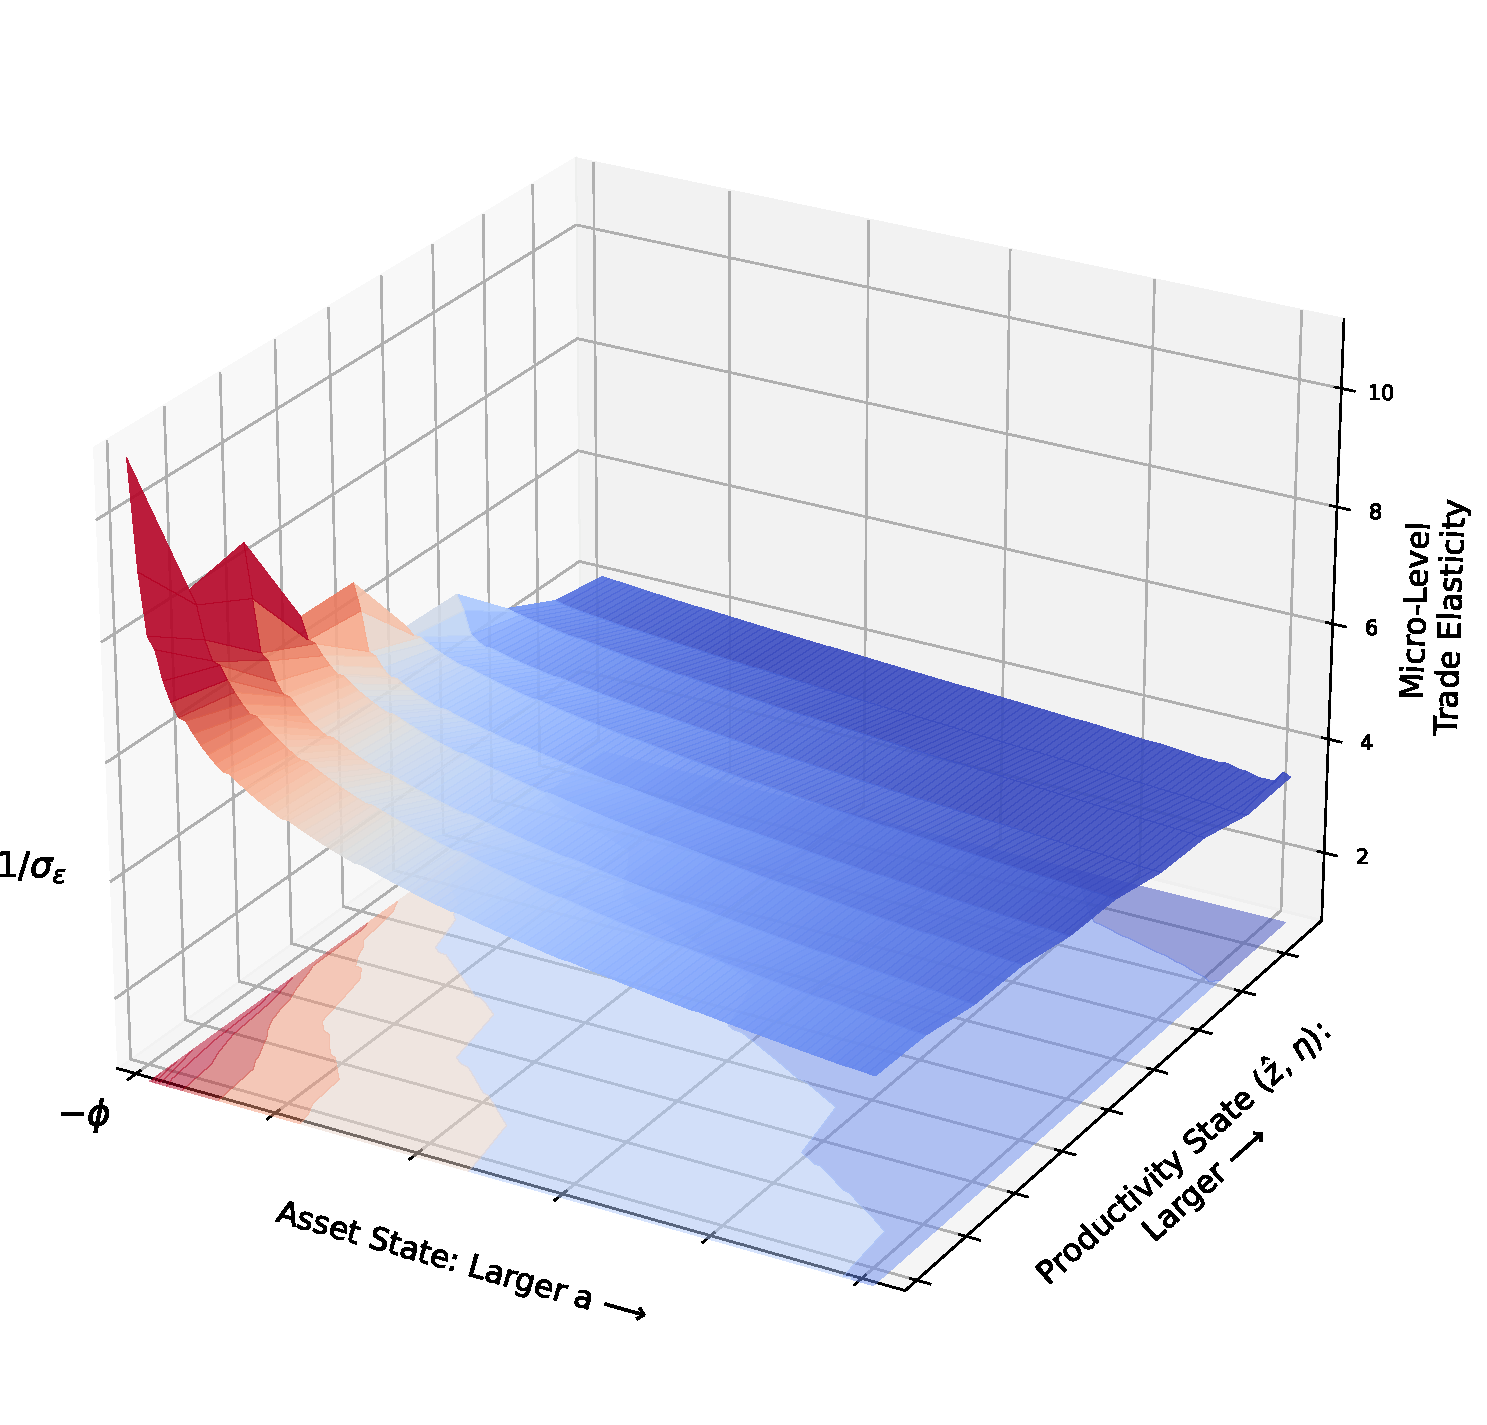
\includegraphics[width = .62\textwidth]{./figures/micro-elasticity.pdf}}
\caption{Elasticities, $-\theta_{ij}(a,z)$}\label{fig:elasticity}
\end{figure}


\begin{figure}[!t]
\centering{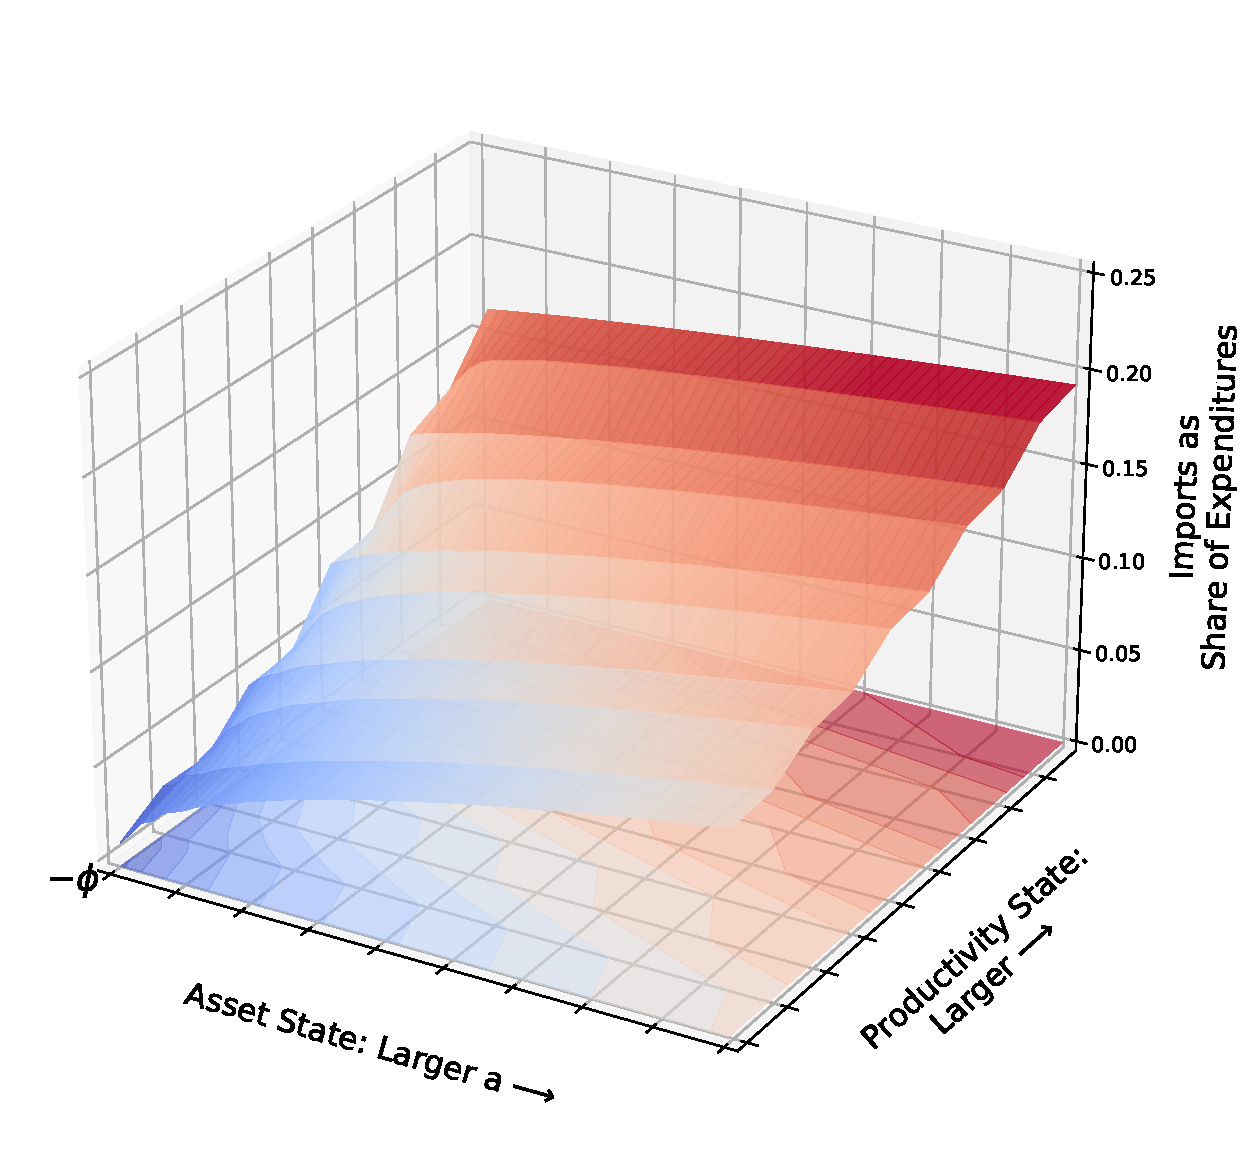
\includegraphics[width = .62\textwidth]{./figures/trade-share.pdf}}
\caption{Trade, $M_{ij}(a,z) / M_{ii}(a,z)$ }\label{fig:micro-trade}
\end{figure}


}

Figure \ref{fig:elasticity} and \ref{fig:micro-trade} illustrates how this works in a two country economy. Figure \ref{fig:elasticity} plots the absolute value of the trade elasticity (intensive and extensive margin) by household state (assets are on the x-axis, productivity state on the y-axis) and the borrowing constraint $\phi$ is in the south-west corner. This shows is how the trade elasticity systematically varies with assets and income: Poor households|especially those near the borrowing constraint|are very price elastic with a trade elasticity of around $-10$. Richer households are less price elastic with this elasticity declining below $-4.$

Because rich and poor households face the same prices, differences in elasticities lead to different trade shares. Figure \ref{fig:micro-trade} plots expenditure on the foreign good relative to the home good. First, note that because of trade costs and symmetry across countries, the home good is the relatively cheaper good. Thus, poor, high-price-elastic households spend more on the home good versus the foreign good. In fact for those near the borrowing constraint in this example, it's near zero. Thus, this is a model where micro-level heterogeneity in trade elasticities leads to micro-level variation in expenditure patterns that vary with assets and income.

This pattern of trade elasticities mimics \citeapos{harrod1936trade} ``Law of Diminishing Elasticity of Demand'' that says that price sensitivity declines with income; see, e.g., \citet{sangani2022markups} who provides evidence in support of this fact and discusses related literature. The evidence in \citet*{auer2022unequal} most closely relates to the patterns in Figure \ref{fig:elasticity} and \ref{fig:micro-trade} in that they find (i) household-level import shares systematically differ between rich and poor (ii) poorer households have higher price elasticities and (iii) rich and poor appear to be facing the same relative price changes.

\subsection{The Gains from Trade}

In this section I compute how social welfare changes due to a permanent change in trade costs. This section derives these gains across steady states, the idea here is that I'm thinking a situation where the change is small and there is an immediate jump to the new steady state. The purpose here is to heuristically illustrate mechanics and where the gains from trade arise from. Unlike the trade elasticity, I take total derivatives that encompass general equilibrium changes in wages and interest rates.

The analysis proceeds in several steps before stating the main result in Proposition \ref{prp:gains-trade}. First, I focus only on country $i$ and study a change in trade costs $d_{ij}$. To simplify the algebra, I choose $w_i$ to be the numeraire and normalize $A_i = 1$. This implies is that $p_{ii}$ equals one and it's derivative with respect to a change in trade costs is zero as it's pinned down by my choice of normalizations.

As in the efficient allocation, I focus on a utilitarian social welfare function:
\begin{align}
W_{i} = \int_{z} \int_{a}  v_{i}(a,z) L_i \lambda_{i}(a,z)
\label{eq:apx-social-welfare}
\end{align}
where $v_{i}(a,z)$ is a households ex-ante (before preference shocks are realized) value function in country $i$, with states $a,z$. The total change in total welfare is
\begin{align}
\frac{\mathrm{d} W_{i}}{\mathrm{d} d_{ij} / d_{ij}} \approx \int_{z} \int_{a} \bigg \{ \frac{\mathrm{d} v_i(a, z)}{\mathrm{d} d_{ij} / d_{ij}}  + v_{i}(a,z) \frac{\mathrm{d} \lambda_{i}(a,z)/ \lambda_{i}(a,z)}{\mathrm{d} d_{ij} / d_{ij}}  \bigg \} L_i \lambda_{i}(a,z).
\label{eq:social-welfare-change}
\end{align}
where the $\approx$ symbol reinforces my point that this is a heuristic, thinking about a small change and there is an immediate jump to the new steady state.

At a high-level, (\ref{eq:social-welfare-change}) illustrates that the gains from trade come through two forces. The first component reflects changes in household-level welfare. So conditional on a distribution of households across states, this computes if households are better (or worse!) off from the change. Relative to the efficient allocation this force is always present, however, the planner equalizes things across households such that individual states do not matter and, thus, distributional issues do not matter.

The second component of (\ref{eq:social-welfare-change}) is about reallocation. It says: take the old $v$'s and compute how the change in the distribution (that arise because of behavioral responses of households) effects social welfare. So does trade make it more or less likely that households are in ``good'' parts of the distribution. This force is unique to the decentralized allocation and symptomatic of an inefficiency in the initial allocation.

In total, the change in social welfare is then the weighted average of these two forces with the weights being those at the initial distribution.

A key issue is how household-level welfare changes. Here, I make the use of the observation in Equation (\ref{eq:log_sum-home}) that the ex-ante value function can be represented in only in terms of home choice $ii$ values and then recursively push forward. In other words, I can compute $\frac{\mathrm{d} v_i(a, z)}{\mathrm{d} d_{ij} / d_{ij}}$ \emph{as if} one only consumed the home good for the infinite future. This observation gives rise to the following:
\begin{align}
\frac{\mathrm{d} v_i(a, z)}{\mathrm{d} d_{ij} / d_{ij}} =& -\sigma_{\epsilon} \frac{\mathrm{d} \pi_{ii}(a,z) / \pi_{ii}(a,z)}{\mathrm{d}d_{ij} / d_{ij}} \ + \ \underbrace{u'(c_{i}(a,z,i))a \ \frac{\mathrm{d} R_{i}}{\mathrm{d} d_{ij} / d_{ij}}}_{\gamma_{ii}(a,z)} \\
\nonumber \\
& + \beta \mathbb{E} \bigg \{ -\sigma_{\epsilon} \frac{\mathrm{d} \pi_{ii}(a',z') / \pi_{ii}(a',z')}{\mathrm{d}d_{ij} / d_{ij}} +  u'(c_{i}(a',z',i))\frac{\mathrm{d} R_{i}}{\mathrm{d} d_{ij} / d_{ij}}a' \ \  \ldots \mbox{and into the future.} \nonumber
\end{align}
Let me walk through the interpretation of each term.\footnote{Similar to Footnote \ref{f-note:bc-elasticity}, a general expression has terms reflecting the effect of borrowing constraints. But again, envelope arguments for small changes mean that these terms are zero.} The first term: $-\sigma_{\epsilon} \frac{\mathrm{d} \pi_{ii}(a,z) / \pi_{ii}(a,z)}{\mathrm{d}d_{ij} / d_{ij}}$ is what I'll call \emph{gains from substitution}. Using logic from \citet{arkolakis2012new}, the change in the home choice probability summarizes the benefits of price changes and, hence, it reflects the gains associated with this substitution.

The second term $u'(c_{ii}(a,z))a \ \frac{\mathrm{d} R_{i}}{\mathrm{d} d_{ij} / d_{ij}}$ is what I'll term as \emph{gains to asset trade}. The idea here is that changes in trade costs affect the equilibrium interest rate in the country and then benefit (or hurt) households depending upon their net asset position.  For example, if a trade liberalization leads to an increase in interest rates, net debtors suffer since their terms to borrow deteriorated, while net savers benefit.

Why might a trade liberalization change interest rates? It's because the liberalization has heterogenous effects on expenditure patterns and savings through the forces discussed in Section \ref{sec:trade-elasticity}. So if the liberalization disproportionately benefits rich /savers in the economy, they shed assets to consume a bit more of the now cheaper goods. Then interest rates must increase to clear financial markets impacting the poor / debtors in the economy. The novelty here is how the goods trade and the financial market are interlinked|not separate as they are typically treated.

Finally, these repeat themselves into the expected future, appropriately discounted. Proposition \ref{prp:gains-trade} summarizes the result below.
\begin{prp}[\textbf{H-A Welfare Gains from Trade}] \label{prp:gains-trade} The welfare gains from trade are given by
{\footnotesize
\begin{align}
\frac{\mathrm{d} W_{i}}{\mathrm{d} d_{ij} / d_{ij}} \approx \int_{z} \int_{a}  \bigg \{ \frac{\mathrm{d} v_i(a, z)}{\mathrm{d} d_{ij} / d_{ij}}  + v_{i}(a,z) \frac{\mathrm{d} \lambda_{i}(a,z)/ \lambda_{i}(a,z)}{\mathrm{d} d_{ij} / d_{ij}}  \bigg \} L_i \lambda_{i}(a,z).
\nonumber
\end{align}
}which reflects the change in household level gains and how the distribution of households changes. Household level gains are given by
{\footnotesize
\begin{align}
\nonumber
\frac{\mathrm{d} v_i(a, z)}{\mathrm{d} d_{ij} / d_{ij}} = \mathbb{E}_{z} \sum_{t = 0}^{\infty} \beta^{t} \bigg \{ -\sigma_{\epsilon} \frac{\mathrm{d} \pi_{ii}(a_{t},z_{t}) / \pi_{ii}(a_{t},z_{t})}{\mathrm{d}d_{ij} / d_{ij}} + u'(c_{i}(a_{t},z_{t},i))a_{t} \times \frac{\mathrm{d} R_{i}}{\mathrm{d} d_{ij} / d_{ij}} \bigg \}
\end{align}
}where each term represents:
\begin{itemize}
\item Gains from substitution: $-\sigma_{\epsilon} \frac{\mathrm{d} \pi_{ii}(a_{t},z_{t}) / \pi_{ii}(a_{t},z_{t})}{\mathrm{d}d_{ij} / d_{ij}}$.

\item Gains to asset trade: $u'(c_{i}(a_{t},z_{t}, i))a_{t} \times \frac{\mathrm{d} R_{i}}{\mathrm{d} d_{ij} / d_{ij}}$
\end{itemize}
\end{prp}

\subsection{The Case of $\log$ preferences}

There is one special case worth working through, it's with $\log$ preferences over the physical commodity. This (very common) preference structure leads to an interesting result where micro-level heterogeneity, market incompleteness completely sperate from the trade side of the economy. So in this one case, trade behaves ``as if'' there were a representative agent Armington-CES consumer and then the gains from trade take the form in \citet{arkolakis2012new}|even though individual households are facing shocks, borrowing constraints, and in general trying to deal with life's circumstances.

Consider the following preference structure:
\begin{align}
\tilde{u}( c_{ij,t} ) =  \log(c_{ij,t}) + \epsilon_{j,t}. \nonumber
\end{align}
There is essentially one insight and then everything follows. Examining the problem in (\ref{eq:value_fun_option}) and substituting in the households budget constraint from (\ref{eq:trade-budget-constraint}), then leads to the observation that the optimal $a'$ conditional on a choice $j$ is \textbf{independent} of the price and the choice $j$. In Appendix \ref{apx-sec:log-preferences}, I employ a formal ``guess and verify'' approach off the Euler equation and show it leads to the same conclusion and this is verified on the computer as well.

Everything follows from this observation.

Because assets don't adjust to changes in prices, from (\ref{eq:intensive-margin}) the intensive margin elasticity for $ij$ is minus one. On the extensive margin, things are more involved as at the micro level they are varying by income and assets. But across different destinations, within states, they vary in the same exact way. Given that the trade elasticity is always defined relative to home choices, heterogenous effects wash out and the end result is that everything collapses to $-\frac{1}{\sigma_{\epsilon}}$. Similarly, aggregate trade satisfies a gravity-like relationship (which no role for household heterogeneity) as in a CES-Armington model or \citet{eaton2002technology}.

Working from Proposition \ref{prp:gains-trade} one can see how the gains only depend on aggregates. The reallocation term in (\ref{eq:social-welfare-change}) is zero because asset holdings don't change. The gains to asset trade are zero because $R$ does not move. Thus, the gains from trade are only about the discounted stream of changes in the home choice probability $\pi_{ii}$|which is the same for rich and poor households per the argument in the previous paragraph.

Appendix \ref{apx-sec:log-preferences} works through this logic step-by-step. Below I state the result:
\begin{corr}[\textbf{Separation of Trade and Micro-Heterogeneity}]\label{prp:seperation} In the dynamic, heterogenous agent trade model where preferences are logarithmic over the physical commodity: The trade elasticity is
\begin{align}
\theta = -\frac{1}{\sigma_{\epsilon}}, \nonumber
\end{align}
and relative trade flows satisfy a gravity relationship
\begin{align}
\frac{M_{ij}}{M_{ii}} = \left( \frac{  w_{j} / A_{j} }{  w_{i} / A_{i} } \right)^{\frac{-1}{\sigma_{\epsilon}}} d_{ij}^{\frac{-1}{\sigma_{\epsilon}}}, \nonumber
\end{align}
and are independent of the household heterogeneity. Ant the welfare gains from trade are
\begin{align}
\frac{\mathrm{d} W_{i}}{\mathrm{d} d_{ij} / d_{ij}} = -\frac{1}{\theta (1-\beta)} \times \frac{\mathrm{d} \pi_{ii} / \pi_{ii}}{\mathrm{d}d_{ij} / d_{ij}}. \nonumber
\end{align}
and is (i) independent of the household heterogeneity and (ii) summarized by the trade elasticity and the change in the home choice probability.
\end{corr}
To be honest, I found this result surprising. By looking at the choice probabilities in (\ref{eq:choice-prob}) and noting how the value functions determine choices, not period utility functions, one would suspect that the household's income fluctuations problem would shape aggregate trade outcomes. Corollary \ref{prp:seperation} shows that is not the case but that micro-outcomes and aggregate trade outcomes ``separate.''

Not only does heterogeneity not matter, aggregate outcomes essentially mimic the results of \citet{arkolakis2012new} and, thus, my heterogenous agent model \emph{with log preferences} delivers the ``same old gains.'' Trade flows take a constant elasticity form with the trade elasticity pinned down by the dispersion parameter on the trade shocks. And then the total change in welfare is summarized by the trade elasticity and how the share of home purchases changes to any change in trade costs.

Proposition \ref{prp:seperation} is also interesting because it generalizes the results of \citet*{anderson1987ces} and \citet{anderson1992discrete} to a far more complicated economy. They showed that in a static model with log utility and additive logit shocks, the economy behaves \emph{as if} there were a representative agent CES consumer. I recover their result, but I must emphasize the complexity of the economy at the micro-level for which this result stands|households are froward looking, face productivity and taste shocks in the presence of incomplete markets and borrowing constraints. Yet, these details don't matter when the magic of $\log$ kicks in.

\section{Calibration}

This section focuses on my approach to calibrating the model.

At a high-level, I follow the gravity literature by picking country specific parameters to match bilateral trade flows. How I do this is a novelty of my paper|I use ``gravity as a guide'' to overcome the fact that my model does not admit a closed form map from trade flows to parameters as static, gravity models do. I describe this approach below and then discuss how the remaining non-country specific parameters are chosen.

In the quantitative work below, I always focus on the case of Financial Globalization where there is a international bond market and a global interest rate.

\subsection{Using Gravity as a Guide}

My calibration strategy is to use the gravity regression as a guide in an indirect inference procedure where I estimate parameters of the model so that the regression coefficients from a standard gravity regression run on my model's data match that seen in the data.

Here are the details. The bilateral trade flows that I use are from \citet{eaton2002technology}. The 19 countries in this data set is about the right size to do what I want to do below in about an afternoon. Moreover, the \citet{eaton2002technology} data set provides a well defined benchmark disciplined by bilateral trade flows and gravity variables|so it's a nice laboratory to explore new issues within.

In the 19 country model, the parameters I need to choose are 19 country-specific TFP parameters (the $A_i$s) and then $(19-1) \times (19-1)$ trade costs (with the minus one since the $ii$ trade costs is normalized to one) to infer from the bilateral trade data. This leaves me under-identified with  $(19-1) \times (19-1)$ bilateral trade shares.

\textbf{Step 0.} Like most of the literature, I'll reduce the number of parameters to estimate by placing a restriction on trade costs and assume they are some function of observable data.  Specifically, I assume that trade costs take the form as in \citet{eaton2002technology} with
\begin{align}
\log d_{ij} = d_{k} + b + l + e_{h} + m_{i},
\label{eq:trade-cost-function}
\end{align}
where trade costs are a logarithmic function of distance, where $d_k$ with $k = 1,2,...,6$, is the effect of distance between country $i$ and $j$ lying in the $k$-th distance interval.\footnote{Intervals are in miles: $[0,375)$; $[375,750)$; $[750,1500)$; $[1500,3000)$; $[3000,6000)$; and $[6000,\mbox{maximum}]$. } $b$ is the effect of a shared border in which $b =1$ if country $i$ and $j$ share a border and zero otherwise. Similarly $l$ is a dummy variable if country's $i$ and $j$ share a language, and $e_{h}$ is a dummy variable for different indicators of European integration. The final part is an importer fixed effect shifting trade costs up or down depending upon the identity of the importer.

At this point, I've reduced the parameter space to the $29$ (or if your not following $6 + 1 + 1 + 2 + 19$) coefficients on the trade cost function rather than the complete matrix of trade costs and then the 19 TFP terms.

\textbf{Step 1.} Then I'm going to run the following gravity regression on the data
\begin{align}
\log \left( {\frac{X_{ij}}{X_{ii}}} \right) = {M_{i}} + {Ex_{j}} + {d_{k}} + {b} + {l} + {e_{h}} + \delta_{ij},
\label{eq:gravity-data}
\end{align}
which projects normalized imports between country $i$ and $j$ on an importer effect, exporter effect and then the gravity variables relating to distance, border, language, etc. and finally there is an error term $\delta_{ij}$ that reflects other factors not in this specification.

This is the canonical representation of trade flows|the gravity model.In a standard Armington-CES, \citet{eaton2002technology}, or \citet{melitz2003impact} style model, the importer effects and exporter effects have specific interpretations. And given the point estimates from (\ref{eq:gravity-data}), productivity and the importer fixed effects on the trade cost function are easily recovered.

In my model, this is not the case. However, what I can do is use the point estimates from (\ref{eq:gravity-data})) as moments for my model to match. Abstracting from normalizations, I now have $19 + 29$ point estimates to match up with the $19 + 29$ parameters I need to estimate.\footnote{To be clear about normalizations: I really only have 18 TFP parameters to match and then a normalization on the importer fixed effects is that they sum to zero as in \citet{eaton2002technology}. The fixed effects in \ref{eq:gravity-data} satisfy the normalization that each of their sum is zero. Thus I have $18 + 28$ parameters to match $18 + 28$ moments}

The next step constructs model analogs to (\ref{eq:gravity-data}).

\textbf{Step 2.} To construct model analogs to (\ref{eq:gravity-data}), I guess a set of $19 + 29$ TFP parameters and coefficients on the trade cost function in (\ref{eq:trade-cost-function}). Define this parameter vector as $\Theta$.

Given $\Theta$, I compute an equilibrium of the world economy. This amounts to: (i) solving for households' dynamic problems|in each country (ii) constructing the stationary distribution of wealth and expenditure patterns|in each country (iii) aggregating and then (iv) finding a vector of prices so goods markets and financial markets clear world wide.

Once I find an equilibrium, I run the same regression as in (\ref{eq:gravity-data}) on the model generated data. As some notation, the model constructed moments are defined as, e.g., $M_{i}(\Theta)$ which is the importer effect estimated on model generated data under the parameter vector $\Theta$.

\textbf{Step 3.} The final step constructs moment conditions which provide the foundation for estimation. Define $\mathbf{y}(\Theta)$ as a set of moments conditions comparing the point estimates from the data with the point estimates from the model under the parameter vector $\Theta$. For example, ${M_{i}} - M_{i}(\Theta)$ or $d_k - d_k(\Theta)$, etc.

My estimation procedure is based on the moment condition
\begin{align}
E\left[\mathbf{y}(\Theta_o)\right] = 0,
\end{align}
where $\Theta_o$ is the true value of $\Theta$. Thus, my method of moments estimator is:
\begin{align}
\hat{\Theta} = \arg\min_{\Theta} \left[\mathbf{y}(\Theta)'\ \mathbf{y}(\Theta)\right], \label{eq:smm-condition}
\end{align}
At a mechanical level, finding the minimum to (\ref{eq:smm-condition}) amounts to returning to \textbf{Step 2.} each time and smartly updating parameter guess for $\Theta$. One of the nice features of this set-up and the dimensionality reduction that I did, is that now this is an exactly identified problem and standard root-finding techniques can be applied to update $\Theta$ and a minimum found.

\begin{figure}[!t]
\centering{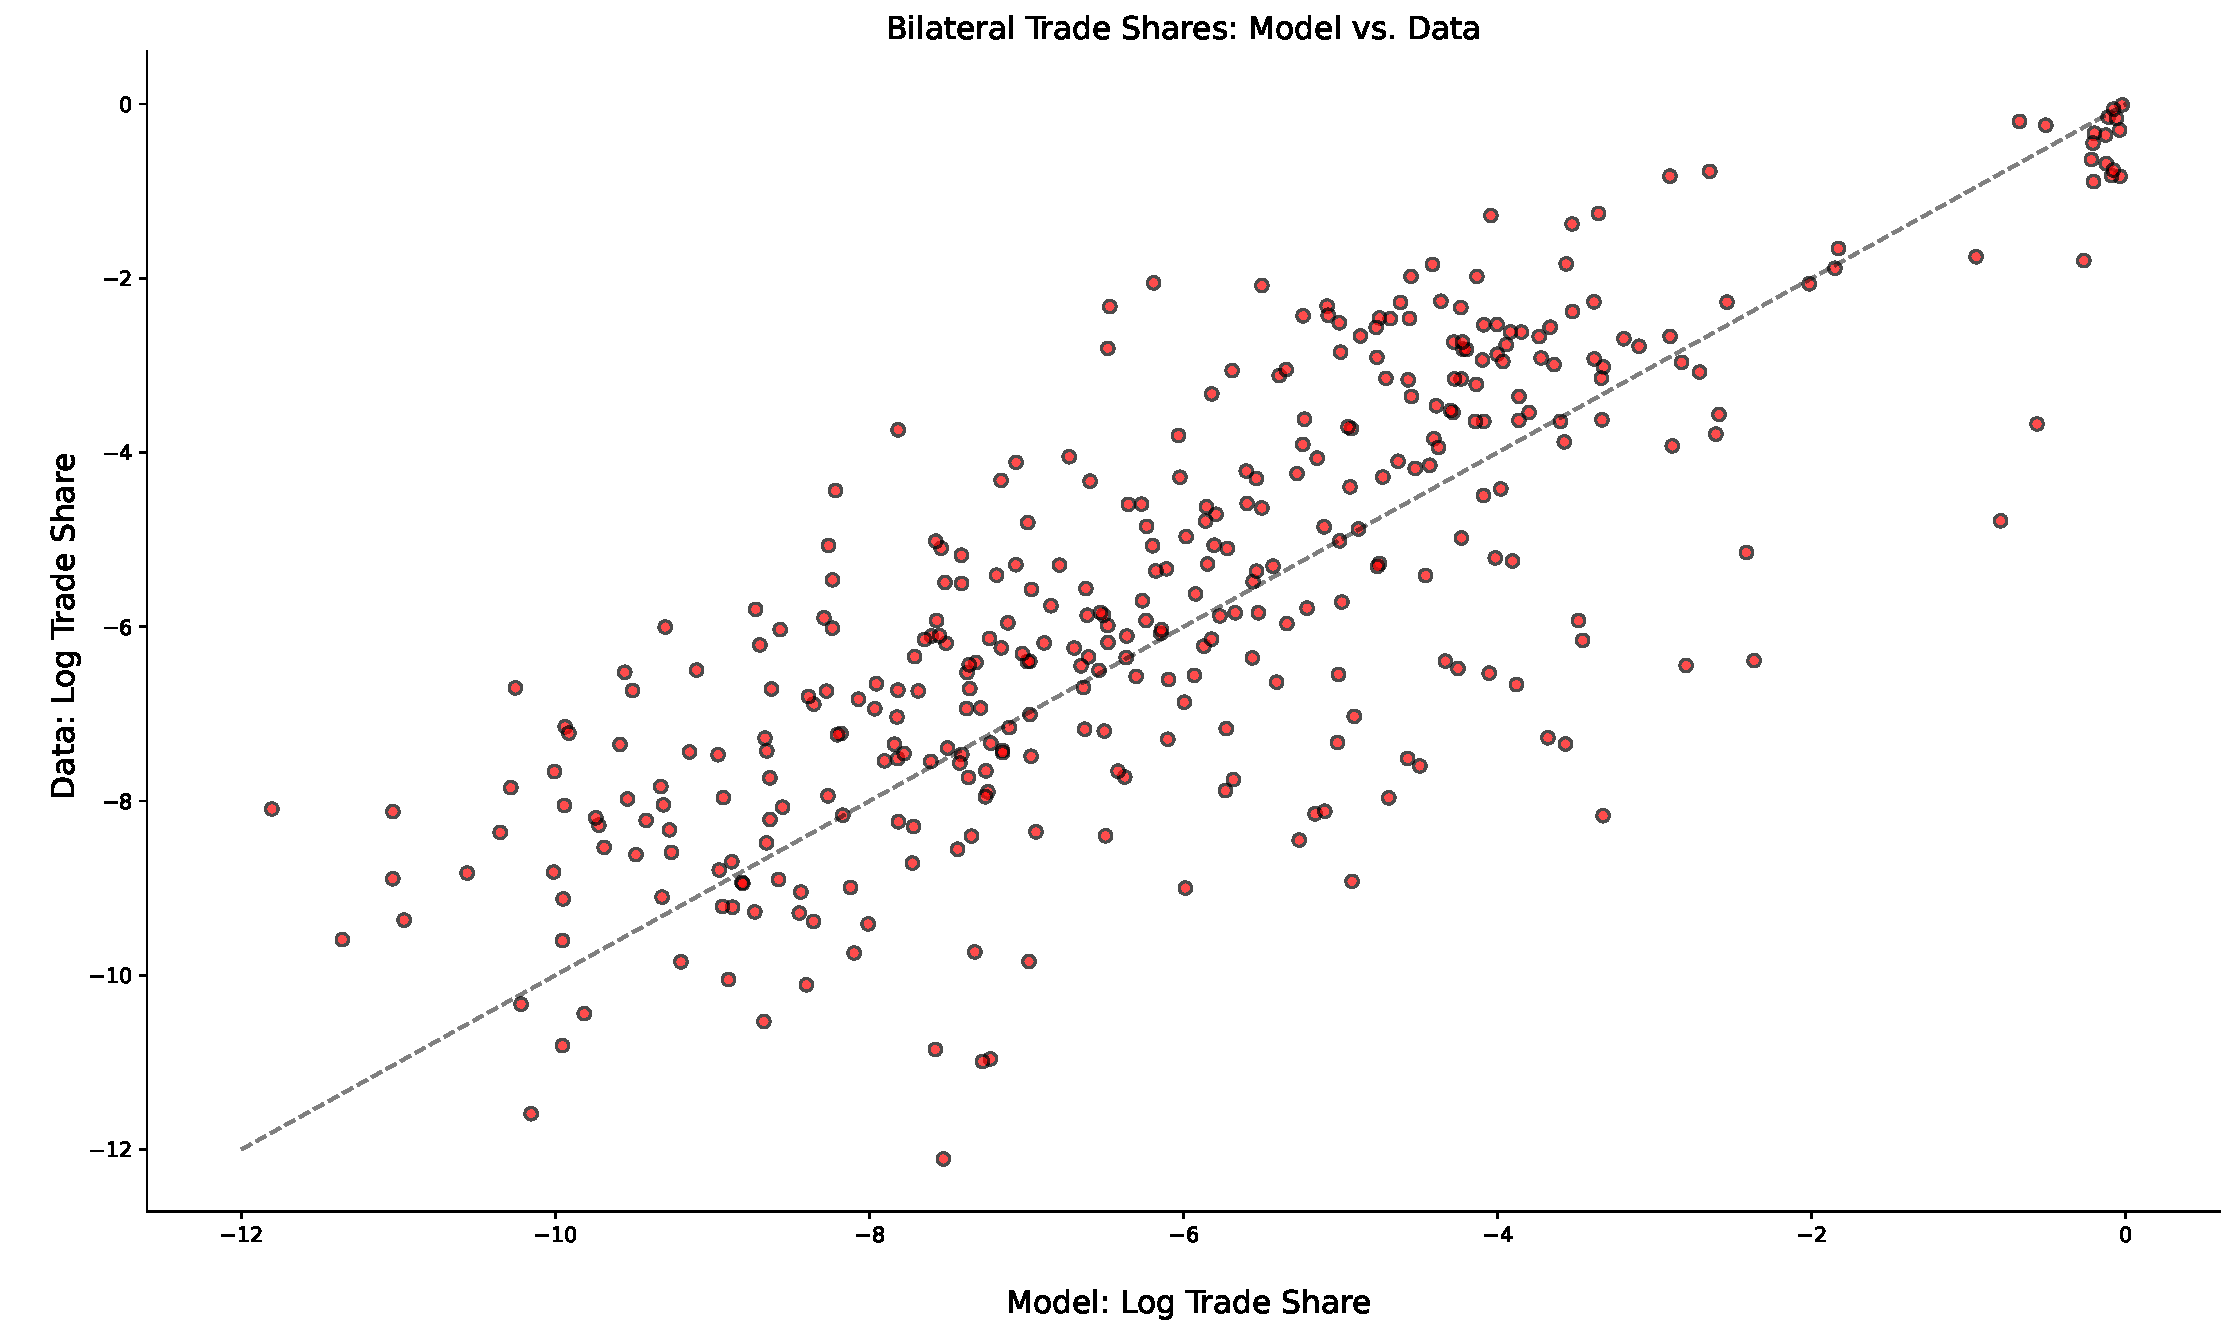
\includegraphics[scale = .45]{./figures/trade-fit.pdf}}
\caption{Bilateral Trade: Model vs. Data}\label{fig:model-fit}
\end{figure}

\subsection{Remaining Parameter Values}

The final parameters to calibrated in the following way. First, utility over the physical commodity is CRRA with relative risk aversion $\gamma =  1.5$, so just a bit above $\log$ and per the discussion above will lead to a pattern (at least qualitatively) or elasticities of substitution across rich and poor households that are consistent with \citet*{auer2022unequal}.

The income shock process is set up to be a mixture of a persistent and transitory component and calibrated as in \citet*{krueger2016macroeconomics}. I use their exact parameter values. And it is assumed to be the same across countries.

The borrowing constraint is set in the following way. First, I scale it by a countries autarky level of average real labor income. Then it is set so that a household can borrow up to fifty percent of it's autarky level of income. The scaling here is done to deliver a ``balanced-growth-like'' property of the model so a households debt capacity is invariant to a country's level of income. Since the level of income is endogenous, a solution to this is to pin things down my connecting it with the autarky labor income.

The discount factor is jiggled around so the equilibrium world interest rate is about 1.5 percent.

The taste shock parameter is set in the following way. First, I set it so that $1 / \sigma_{\epsilon} = 4.0$. Second, I then scale this parameter country by country to deliver a ``balanced-growth-like'' property of the model. Specifically, each country will have it's own parameter and it is scaled so that $\sigma_{\epsilon,i} = \sigma_{\epsilon} A_i^{1-\gamma}$. What this implies is that if there were two countries  one with high TFP and one with low TFP in a closed economy, this scaling ensures that trade elasticities in the two countries are the same, but one is just richer than the other.

\subsection{Calibration Results}

Figure \ref{fig:model-fit} provides a sense of model fit after running my ``gravity as guide procedure.'' The y-axis reports bilateral trade data and the x-axis reports the outcome from my model. The fit is very high, and nearly indistinguishable from, for example, how a standard trade model perform would perform. Or the $\log$ preference model which per Proposition \ref{prp:seperation} should (and it does) operate just like a standard trade model.

Table \ref{tb-grav-est} reports another measure of fit and some of the resulting parameter values. The first column are the distance, border, etc. moments from the gravity regression in (\ref{eq:gravity-data}) (and note they exactly correspond with those in the top panel of Table 3 of \citet{eaton2002technology}). The second column reports the moments from the model. Here they exactly line up and are consistent with the argument in Figure \ref{fig:model-fit}, the fit is good and the model is replicating geographic pattern of activity seen in the data.

\begin{table}[t]
\small
\begin{center}
\refstepcounter{table}
\setlength {\tabcolsep}{5.5mm}
\renewcommand{\arraystretch}{1.50}\label{tb-grav-est}
\begin{tabular}[t]{l c c c}
\multicolumn{4}{c}{{\normalsize\textbf{Table \ref{tb-grav-est}: Estimation Results}} }
\\\hline \hline
& & \multicolumn{2}{c}{\textbf{HAT-Model}}  \\
\cmidrule(lr){3-4}
Barrier& Moment & Model Fit & Parameter \\
\hline $[0,375)$                &$-3.10 $           & $-3.10 $              & $2.35$           \\
$[375,750)$                     &$-3.67 $           & $-3.67 $              & $2.81$           \\
$[750,1500)$                    &$-4.03 $           & $-4.03 $              & $3.09$           \\
$[1500,3000)$                   &$-4.22 $           & $-4.22 $              & $3.23$           \\
$[3000,6000)$                   &$-6.06 $           & $-6.06 $              & $4.88$           \\
$[6000,\mbox{maximum}]$         &$-6.56 $           & $-6.56 $              & $5.69$           \\
Shared border                   &$\phantom{-}0.30$  & $\phantom{-}0.30$     & $0.91$  \\
Language                        &$\phantom{-}0.51$  & $\phantom{-}0.51$     & $0.87$  \\
EFTA                            &$\phantom{-}0.04$  & $\phantom{-}0.04$     & $0.98$  \\
European Community              &$\phantom{-}0.54$  & $\phantom{-}0.54$     & $0.89$  \\
\hline
\end{tabular}
\\[0.5ex]
\parbox{5.0in}{\footnotesize \textbf{Note:} The first column reports data moments the HAT-model targets. The second reports the model moments. The third column reports the estimated parameter values.}
\end{center}
\end{table}

The final column reports the primitive estimates on the trade cost function. Each value reports the level effect of being in a distance bin or sharing a border etc.  So if two countries are measured to be in the smallest distance bin and share a border, the trade cost between these two countries is $2.35 \times 0.91$ (first row times seventh row). Or if a country is in the furthest distance bin, its trade costs is 5.69.

How would this compare to a standard model? It's a bit hard since one needs to take a stand on the trade elasticity in the standard model to translate estimates in column one into levels of the trade costs. But an approach is the following: find the trade elasticity so the cost of the nearest distance bin is the same as in my model and then look at how things relate in other bins. In an \citet{eaton2002technology} world, this would correspond with an trade elasticity of about 3.6. Then, for example, one takes the moment in the first column, last distance bin and compares $\exp( - 1 / 3.6 \times  -6.56)$ vs. 5.69.

What comes out of is that closer relationship are a bit more expensive then what a constant elasticity model would predict. And the furthest destinations are meaningfully less expensive, seven and ten percent less, for the last two distance bins. This is picking up a model outcome where trade elasticities are increasing with cost. So far away destinations are relatively elastic destinations, so the cost need not be as large to deter trade.

Figure \ref{fig:bilateral-elasticities} provides an example of the of trade elasticities that come of this model. In this figure, I focus on the US and plot each bilateral trade elasticity vs. that countries price in the US. The balls represent the relative size of US imports from that destination. And these elasticities are constructed from the bottom up via the formula in (\ref{eq:trade-elasticity}). The feature that stands out very clearly is that trade elasticities systematically increase with price and decrease with the volume of trade.

\begin{figure}[!t]
\centering{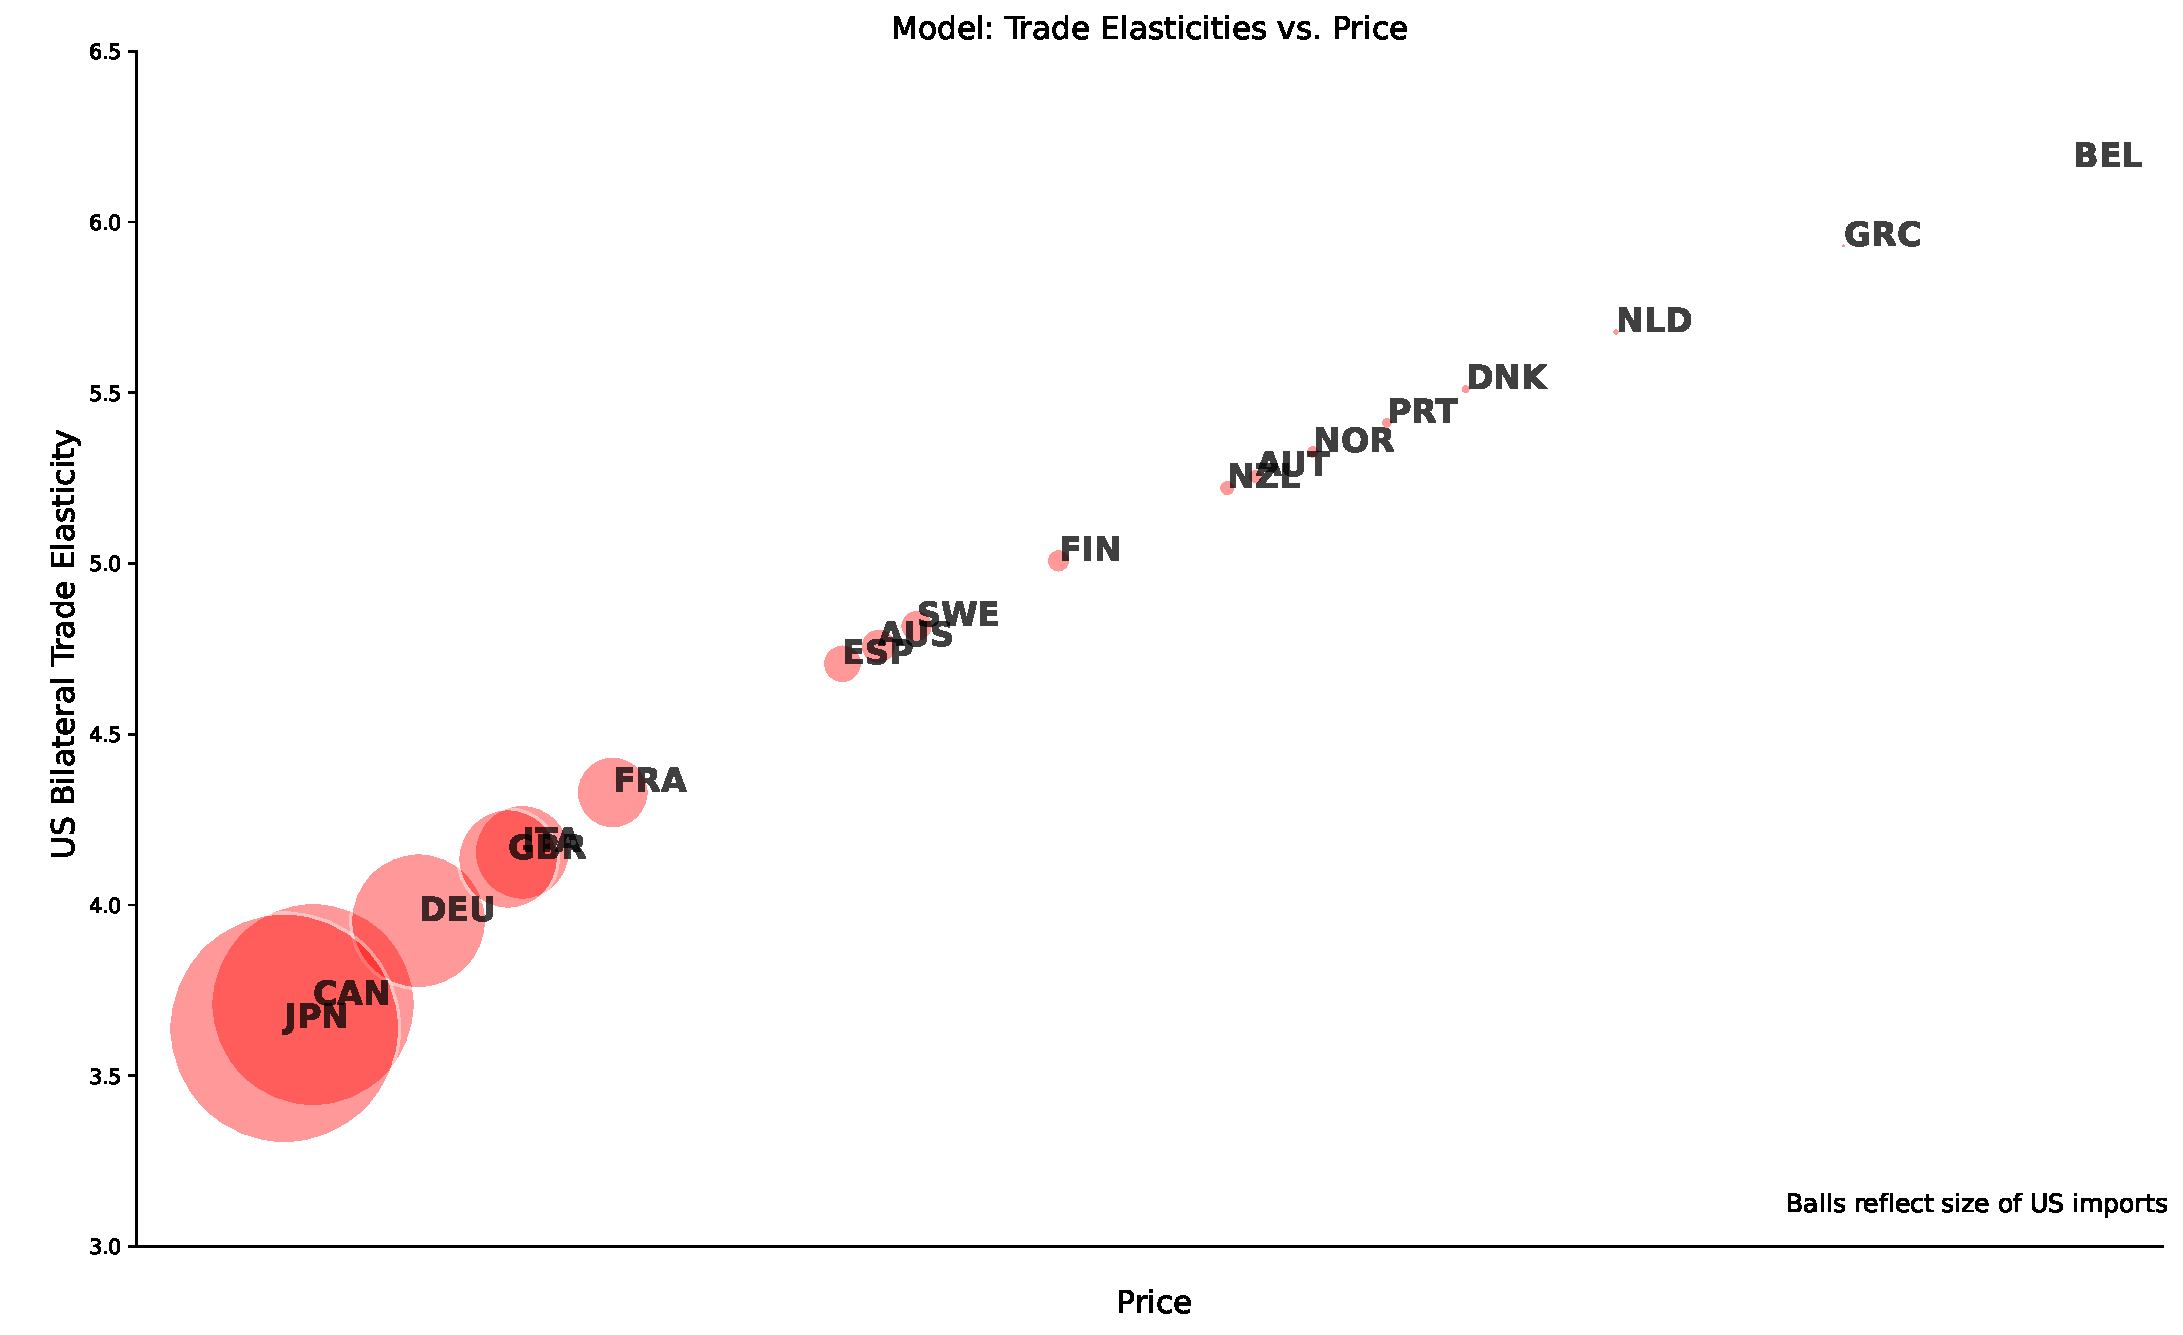
\includegraphics[scale = .45]{./figures/us-elasticity.pdf}}
\caption{Trade Elasticities $-\theta_{us,j}$}\label{fig:bilateral-elasticities}
\end{figure}


At the micro-level, there are two opposing forces giving rise to this aggregate relationship. Per the arguments discussed above around Proposition \ref{prp:GET}, the aggregate bilateral trade elasticity reflects both household level elasticities $\theta(a,z)$s and composition through the expenditure weights $\omega(a,z)$s. Thus, when prices increase as one moves from one source to a less competitive source, there are two competing forces at work: (i) how do micro-level elasticities change and (ii) how does composition change?

The first force is that as prices increase \emph{both} rich and poor households' elasticities increase. In other words, everyone is more elastic when contemplating a purchase from a more expensive destination. This is a force pushing the model to have elasticities \emph{increase} with price.

The second force | the composition effect| generally works in the opposite direction. As one moves from more cheaper to more expensive destinations, less price sensitive households sort into those varieties. Thus, the composition of households purchasing more expensive varieties are the rich, relatively inelastic households. This is a force pushing the model to have elasticities \emph{decrease} with price. In more standard, BLP-like settings, \citet{nakamura2010accounting} and \citet*{head2021poor} highlight this composition effect in shaping pass-through.

Which one wins? Figure \ref{fig:bilateral-elasticities} shows that the first force dominates the composition effect. One way to view this result is through the lens of \citeapos{mrazova2017not} language that demand in this model endogenously turns out to be ``subconvex'' relative to CES demand and which is equivalent to ``Marshall's Second Law of Demand.'' The endogenous part is important as it's not parameterized as in, say, Kimball Demand which has become a popular tool to allow for non-constant elasticities. Did the model have to deliver this? Per the arguments above, it's not obvious as composition effects could have dominated.\footnote{\citet{head2021poor}, using \citeapos{berry1995automobile} estimated model, illustrate that composition does indeed dominate with pass-through greater than one when heterogeneity in the valuation of product characteristics are shut down.}

In the trade literature, there is evidence suggesting that trade elasticities conform to what comes out of my model. Both \citet{novy2013international} and \citet*{carrere2020gravity} find that proxy's for the trade elasticity are larger, the less trade there is between two countries. \citet{chen2022gravity} further confirm this idea by finding that trade cost effects are strong for small bilateral relationships weak or even zero for large trading relationships. Mapping these ideas back into outcomes from my model, a currency union between the US and Canada would likely have a small effect since this is a high volume / low elasticity relationship.



%``super-elasticity'' of trade within the model \emph{endogenously} delivering the result that elasticities increases with price.





\section{Gains From Trade}

Sorry, I'm still filling this in.

\section{Trade in the Efficient Allocation}

This section computes what the pattern of trade \emph{should} look like were we living in a first-best world.

\begin{figure}[!t]
\centering{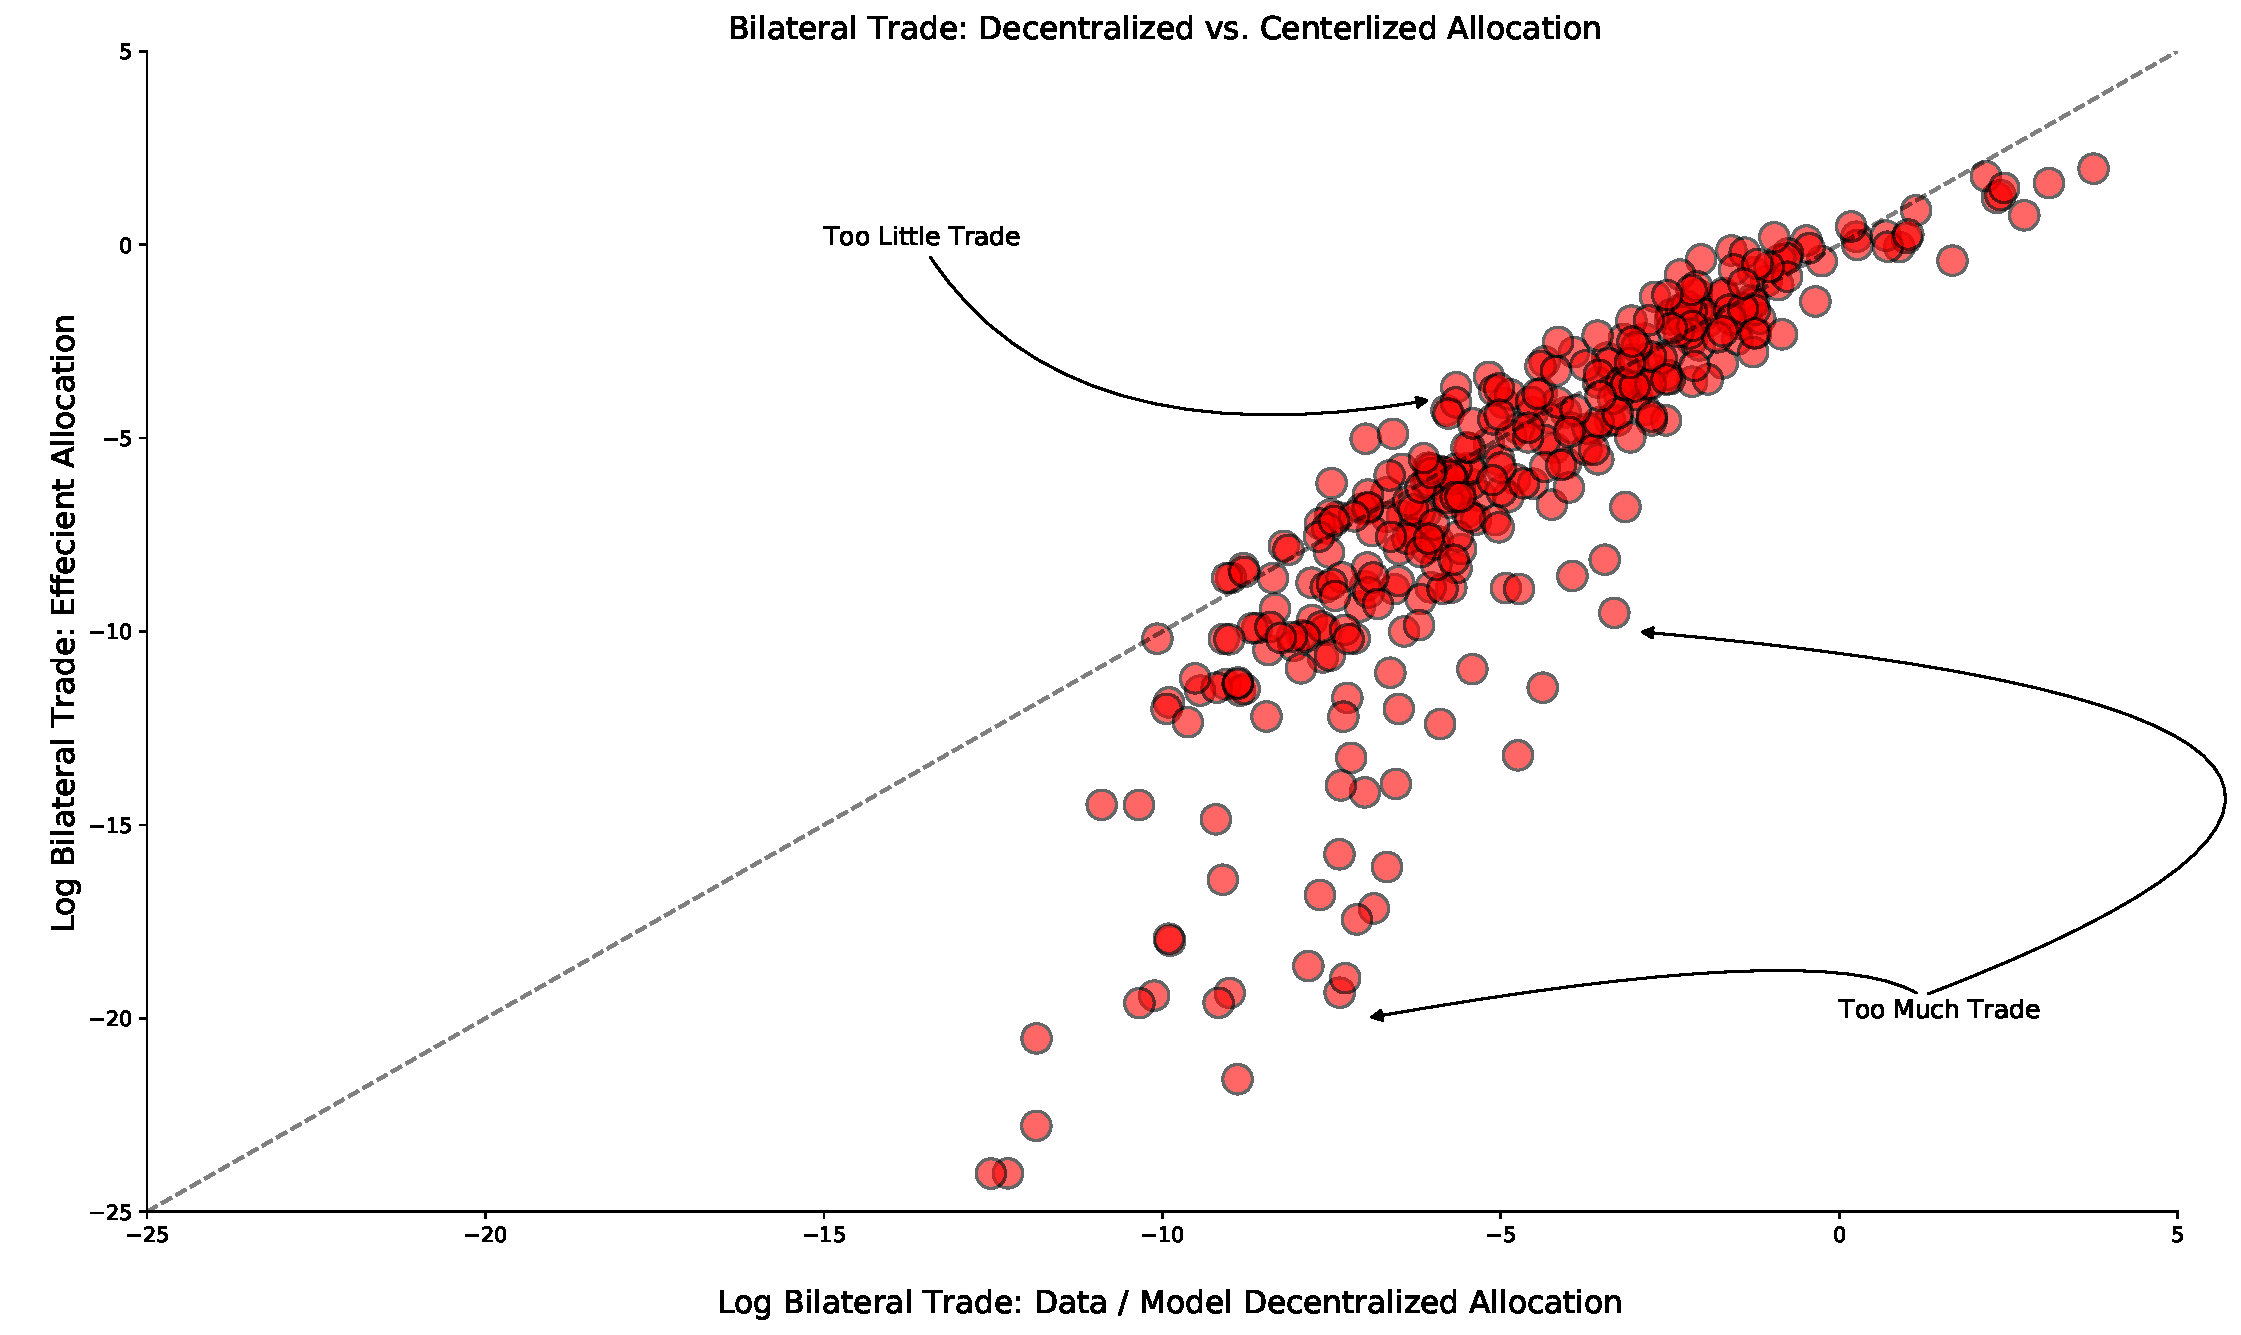
\includegraphics[scale = .45]{./figures/decentralized-trade-all.pdf}}
\caption{}\label{fig:planner-trade}
\end{figure}

Before getting into the results, an important input into computing the allocation in Proposition \ref{prp:efficient-allocation} are the Pareto weights. I set the Pareto weight for a country to be proportional to it's level of TFP. My rationale behind this choice of weights is to eliminate the Planners incentives to shift consumption across countries vs. margins within the country. More specifically, this specification limits the planners desire to redistribute consumption from say, the US (a rich country) to Greece (a poor country in the data set) and focuses the exercise on within country redistribution.

Given the Pareto weights, I take the parameters of the model and then compute consumption allocations and trade flows that solve planning problem described in Section \ref{sec:planner}. To be clear, there is no change in trade costs | all the planner is doing is redistributing and overcoming market incompleteness that is present in the decentralized allocation.

\subsection{Efficient Trade}

Figure \ref{fig:planner-trade} illustrates what the pattern of trade should look like from the planners perspective. The x-axis of Figure \ref{fig:planner-trade} plots log bilateral trade flows in the model (and data) in the decentralized equilibrium. So the same thing as in Figure \ref{fig:model-fit}. The y-axis reports the trade flows in the efficient allocation. The 45-degree line is drawn so if the red-dots lie on this line, this means that trade in the efficient allocation lines up with the decentralized allocation.

Generally they do not line up on the 45-degree line. Two types of deviations stand out. First, small trade flows tends to be made smaller. From the planners perspective these are not efficient trading relationships. In contrast, large trading relationships are generally not large enough, this is the set of dots lying from about -5 to 0. So there is a meaningful sense that the Planner wants a reallocation of how households source goods.

Figure \ref{fig:planner-vs-data} further illustrates this reallocation by focusing on how US imports change. The left panel reports import shares in the model (and data). Here you can see that the aggregate import share is about 7 percent with Canada, Japan, and some other European countries contributing to the bulk of US imports.

In the efficient allocation the planner simultaneously wants the US to trade \emph{more}, but concentrate US imports on it's most productive (and large) partner which is Japan, a bit more from Germany, and less from Canada. And small trade flows with the potpourri of the remaining countries are made much smaller consistent with Figure \ref{fig:planner-trade}.

The issue is this: uncompetitive source countries are ``luxuries'' from the planners perspective. In the decentralized equilibrium, the varieties from these countries are only purchased from rich households (and have the appearance of being luxuries as they are also high elasticity goods). Then, when the planner equalizes consumption within a country, the demand for these goods is eliminated.

Why does trade expand in certain directions? There is an optimistic message here: the US is under-utilizing other productive countries via trade as a means to increase consumption for the masses. This is why trade expands with Japan which in the calibrated economy is very productive with a large labor force.

\begin{figure}[!t]
\begin{subfigure}{0.5\textwidth}
    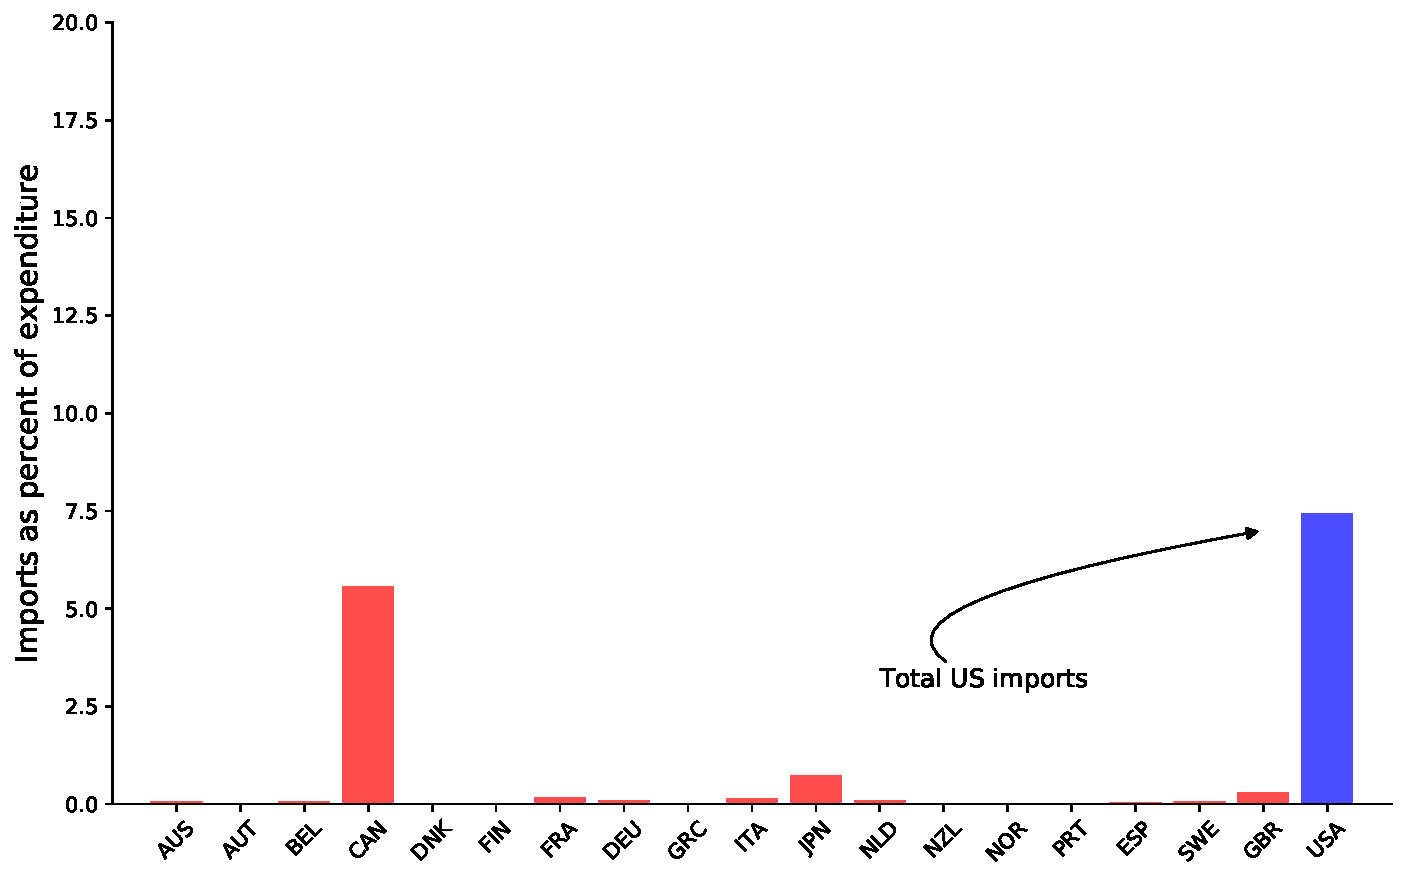
\includegraphics[scale = 0.36]{./figures/decentralized-trade-us.pdf}
    \caption{{Trade in the Decentralized Allocation}}\label{fig:us-data-trade}
\end{subfigure}
\hspace{0.01cm}
\begin{subfigure}{0.5\textwidth}
    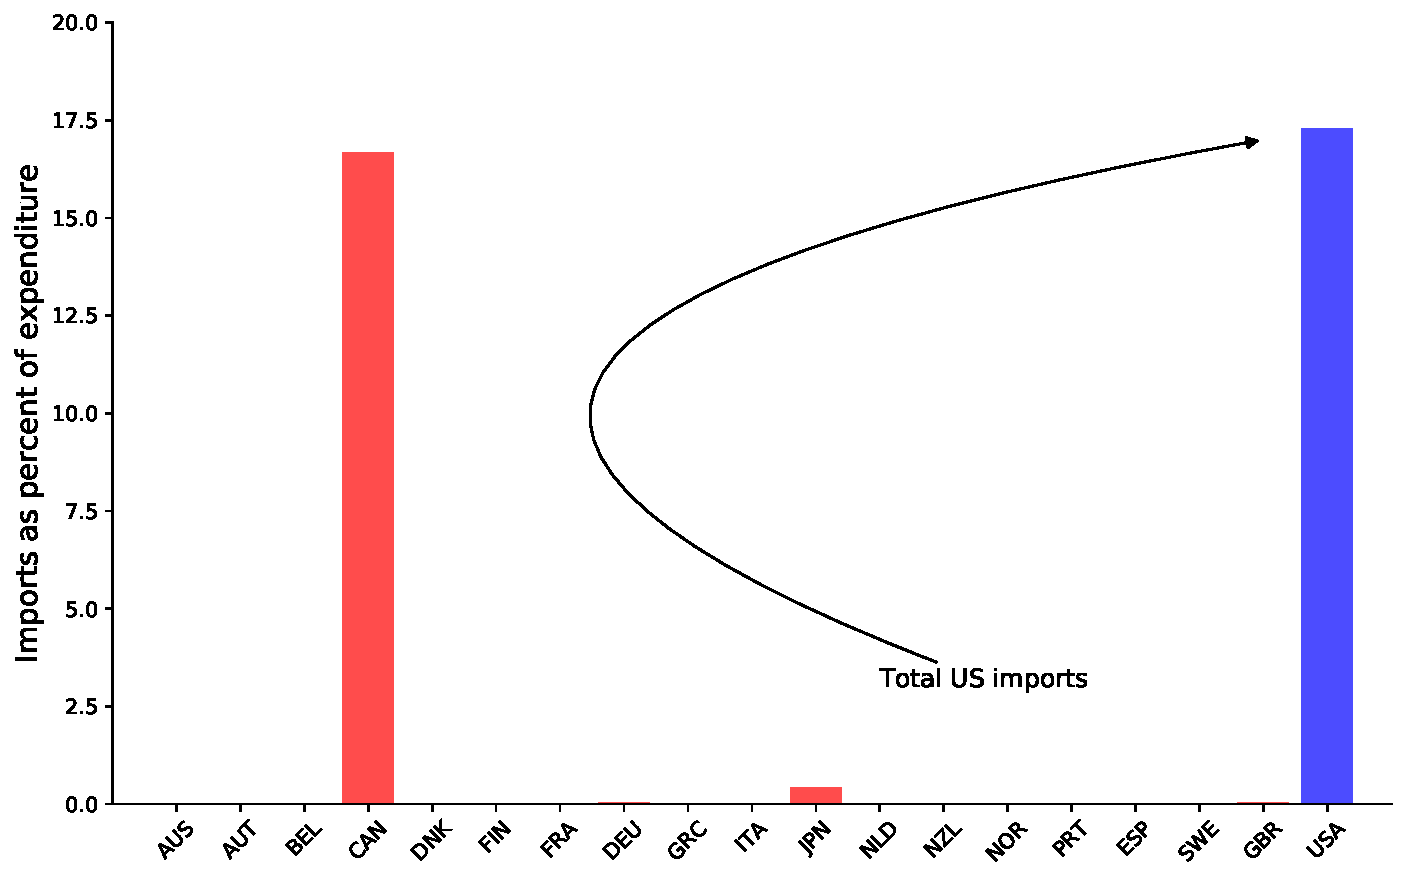
\includegraphics[scale = 0.36]{./figures/planner-trade-us.pdf}
    \caption{{Trade in the Efficient Allocation}}\label{fig:us-planner-trade}
\end{subfigure}
\caption{US imports: Decentralized vs. Centralized Pattern of Trade}\label{fig:planner-vs-data}
\end{figure}


\section{Conclusion}

What do you find interesting? Email me.



\appendix

\clearpage
\newpage

\begin{center}
\textbf{\Large Appendix}
\end{center}

\addcontentsline{toc}{section}{Appendices}

\section{The Planning Problem}\label{sec:apx-planner}

I focus on a utilitarian social welfare function with Pareto weights that vary across countries:
\begin{align}
W = \sum_{t=0}^{\infty} \sum_{i}  \int\limits_{z} \beta^{t} \psi_{i} v_{i}(z,t) L_{i}\lambda_{i}(z,t),
\label{eq:apx-social-welfare}
\end{align}
and here $v_i$ a households utility in country $i$ and $\psi_{i}$ is the Planners weight on those residing in country $i$. Now, I'm going to place the social welfare function in sequence space and then unpack the benefits from the preference shock in the following way:
\begin{align}
W = \sum_{t=0}^{\infty}  \sum_{i}  \sum_{j}  \int\limits_{z}  \beta^{t} \  \psi_{i} \bigg \{  u(c_{ij}(z, t) ) + \mathrm{E}[ \ \epsilon \ | \ \pi_{ij}(z,t) ] \bigg \}\pi_{ij}(z,t) L_{i} \lambda_{i}(z, t)
\label{eq:apx-social-welfare-2}
\end{align}
so the inner term is period utility given the associated consumption allocation $c_{ij}$ and then the expected value of the preference shock conditional on the choice probability $\pi_{ij}(z,t)$. This inner term is then weighted by the number of households that receive that utility, i.e. the choice probability times the mass of households with shock $z$ at date $t$. The sum across $j$ adds up all households in country $i$ and all of this is weighted by the Pareto weight $\psi_{i}$. Then the sum across $i$ reflects that this is global welfare.

One more point about the inner term in (\ref{eq:apx-social-welfare-2}), my claim is that with the Type 1 extreme value shocks:
\begin{align}
\mathrm{E}[ \ \epsilon \ | \ \pi_{ij}(z,t) ] = -\sigma_{\epsilon} \log \pi_{ij}(z,t)
\end{align}
where this is like the ``selection correction'' where if $\pi$ becomes smaller, the expected value of the taste shock becomes larger. So only those with the largest relative shocks are chosen and higher utility for those, conditional on being selected, is felt.

Given this formulation, the planner does the following: he chooses consumption and choice probabilities for all country pair combinations, state by state, for the infinite future. The Lagrangian associated with the Planning Problem is:
\begin{align}
\mathcal{L}  = & \sum_{t=0}^{\infty}   \sum_{i} \sum_{j} \int\limits_{z}  \beta^{t} \ \psi_{i} \bigg \{  u(c_{ij}(z, t) ) + \mathrm{E}[ \ \epsilon \ | \ \pi_{ij}(z,t) ] \bigg \}\pi_{ij}(z,t) L_{i} \lambda_{i}(z, t), \\
\nonumber \\
&+ \sum_{t=0}^{\infty} \sum_{i} \beta^{t} \chi_{i}(t) \bigg \{ Y_{it} \  - \ \sum_{j} \int\limits_{z}  d_{ji} c_{ji}(z, t) \pi_{ji}(z,t) L_{j}\lambda_{j}(z, t) \bigg \} \nonumber \\
\nonumber \\
&+ \sum_{t=0}^{\infty} \sum_{i} \int\limits_{z}  \beta^{t} \chi_{2i}(z,t) \bigg \{1 - \sum_{j}\pi_{ij}(z,t) \bigg \} L_{i} \lambda_{i}(z, t), \nonumber
\label{eq:planning-problem}
\end{align}
where the first term is the objective function; the second line is the resource constraint saying that output from country $i$ must equal the consumption of commodity $i$ globally including the transport costs. Then the third line ensures that choice probabilities are probabilities and sum to one. The final thing I'm doing is that I'm scaling the multipliers by $\beta^t$ so that the algebra is easier.

Associated with this problem are two first order conditions. The first one is consumption in $i$ with respect to variety $j$ so:
\begin{align}
\frac{\partial \mathcal{L} }{\partial c_{ij}(z, t)} &=  \beta^{t} \psi_{i} u'(c_{ij}(z, t))  \pi_{ij}(z,t) L_{i} \lambda_{i}(z, t) - \beta^{t} \chi_{j}(t) d_{ij} \pi_{ij}(z,t) L_{i} \lambda_{i}(z, t) = 0 \\
\nonumber \\
& \Rightarrow \ \ \psi_{i} u'(c_{ij}(z, t) ) = \chi_{j}(t) d_{ij}, \label{apx-eq:muc}
\end{align}
which says that the weighted marginal utility of consumption of ($i$ consuming variety $j$) should equal it's costs. What is this cost, it's the $j$'s multiplier adjusted by the trade cost $d_{ij}$ which gives this ``price'' like interpretation of the multiplier. It's like the shadow value of commodity $j$ which reflects how scarce or not the commodity is then multiplied by the transport costs.

This first order condition has several implications. First, because the right hand size is independent of $z$, then $\psi_{i} u'(c_{ij}(z, t)) = \psi_{i} u'(c_{ij}(z', t)) = \psi_{i} u'(c_{ij}(t))$ for all $z, z'$ combinations. So within choice, the marginal utility of consumption is equated. Second, across variety choice, within a country (so Pareto weights cancel), the ratio of marginal utility across variety $j$ is:
\begin{align}
\frac{u'(c_{ij}(t))}{u'(c_{ij'}(t))} = \frac{\chi_{j}(t) d_{ij}}{\chi_{j'}(t) d_{ij'}}
\end{align}
which says that consumption differences relate to the ratio of the multipliers on the resource constraint and the trade costs. This again gives the price like interpretation of the multipliers, i.e. that differences in the ratio of the marginal utility of consumption reflect relative scarcity or the shadow values. This is essentially a within country \citet{backus1993} condition.

The second first order condition is with respect to the choice probabilities. So
\begin{align}
\frac{\partial \mathcal{L} }{\partial \pi_{ij}(z, t)} \ = \ & \beta^{t} \psi_{i} \bigg \{  u(c_{ij}(z, t) ) + \mathrm{E}[ \ \epsilon \ | \ \pi_{ij}(z,t) ] \bigg \} L_{i} \lambda_{i}(z, t) + \beta^{t}\psi_{i} \frac{\partial \mathrm{E}[ \ \epsilon \ | \ \pi_{ij}(z,t) ]}{\partial \pi_{ij}}\pi_{ij}(z,t) L_{i} \lambda_{i}(z, t) \nonumber \\
\nonumber \\
& - \beta^{t} \chi_{j}(t) d_{ij} c_{ij}(z, t) L_{i}\lambda_{i}(z, t) - \beta^{t} \chi_{2i}(z,t) L_{i} \lambda_{i}(z, t)  = 0
\end{align}
where the first two terms are the marginal, social benefit of changing the choice probabilities. This reflects how utility shifts by adding more households to that choice and then how the expected preference shock changes. The last two terms reflect the costs of changing the choice probabilities which are the resources to provide the additional consumption and the cost of moving households out of other choices which is what the multiplier $\chi_{2i}(z,t)$ represents.

Further simplifying gives:
\begin{align}
\frac{\partial \mathcal{L} }{\partial \pi_{ij}(z, t)} \ = \ &  \psi_{i} \bigg[ u(c_{ij}(z, t) ) + \mathrm{E}[ \ \epsilon \ | \ \pi_{ij}(z,t) ] + \frac{\partial \mathrm{E}[ \ \epsilon \ | \ \pi_{ij}(z,t) ]}{\partial \pi_{ij}} \pi_{ij}(z, t) \bigg] - \chi_{j}(t) d_{ij} c_{ij}(z, t)  - \chi_{2i}(z,t)  = 0.
\end{align}
Then inserting the observations made above about the Type 1 extreme value distribution and then connecting things with the consumption allocation in \ref{apx-eq:muc} one has
\begin{align}
\psi_{i} \bigg[ u(c_{ij}(t) ) -\sigma_{\epsilon} \log \pi_{ij}(z,t) - \sigma_{\epsilon} - u'(c_{ij}(t) )c_{ij}(t)\bigg]   = \chi_{2i}(z,t).
\end{align}
Then some algebra gets toward a closed-form expression for the choice probability
\begin{align}
-\sigma_{\epsilon} \log \pi_{ij}(z,t) = -u(c_{ij}(t)  ) + u'(c_{ij}(t) )c_{ij}(t)  + \sigma_{\epsilon} + \chi_{2i}(z,t)\psi_{i}^{-1}, \\
\nonumber \\
\pi_{ij}(z,t) = \exp \left( \frac{u(c_{ij}(t)  ) - u'(c_{ij}(t))c_{ij}(t)}{\sigma_{\epsilon}} - 1 \right) \bigg / \exp \left( \chi_{2i}(z,t)\psi_{i}^{-1} / \sigma_{\epsilon} \right).
\end{align}
The choice probabilities must sum to one, so we can set the multiplier so
\begin{align}
\exp \left( \chi_{2i}(z,t) \psi_{i}^{-1} / \sigma_{\epsilon} \right) = \sum_{j'}\exp \left( \frac{u(c_{ij}(t)) - u'(c_{ij}(t))c_{ij}(t)}{\sigma_{\epsilon}} - 1 \right),
\end{align}
which implies
\begin{align}
\chi_{2i}(z,t) = \sigma_{\epsilon}  \psi_{i} \log \bigg \{ \sum_{j'}\exp \left( \frac{u(c_{ij}(t)) - u'(c_{ij}(t))c_{ij}(t)}{\sigma_{\epsilon}} - 1 \right) \bigg \}.
\end{align}
Then the choice probability is
\begin{align}
\pi_{ij}(t) =\exp \left( \frac{u(c_{ij}(t)) - u'(c_{ij}(t))c_{ij}(t)}{\sigma_{\epsilon}}\right) \bigg / \sum_{j'}\exp \left( \frac{u(c_{ij'}(t)) - u'(c_{ij'}(t))c_{ij'}(t)}{\sigma_{\epsilon}} \right),
\end{align}
which is independent of $z$ and the Pareto weight does not appear.  This has the standard Type 1 shape, but the inner most term says that the choice probability should reflect the ``net'' social benefit of having someone chose that good. The net part is the utility a household receives net of the cost of providing that amount of the consumption. And the cost is, well, $c$ converted into utils which is what the marginal utility bit is doing. Because of that this is all net, the Pareto weight does not directly appear. Given this discussion, the multiplier $\chi_{2i}(t)$ has the interpretation as the expected, net contribution to social welfare of households in country $i$.

The formal statement is below:
\begin{prp}[\textbf{The Efficient Allocation}]\label{apx-prp:efficient-allocation} The allocation that satisfies the Centralized Planning Problem in (\ref{eq:planner_problem}) is:
\begin{enumerate}
\item A consumption allocation satisfying:
\begin{align}
\psi_{i} u'(c_{ij}(z,t) ) = \chi_{j}(t) d_{ij}
\label{apx-eq:planner-consumption}
\end{align}
where $\chi_{j}(t)$ is the shadow price of variety $j$.
\item The choice probabilities are
\begin{align}
\pi_{ij}(t) =\exp \left( \frac{u(c_{ij}(t)) - u'(c_{ij}(t))c_{ij}(t)}{\sigma_{\epsilon}}\right) \bigg / \sum_{j'}\exp \left( \frac{u(c_{ij'}(t)) - u'(c_{ij'}(t))c_{ij'}(t)}{\sigma_{\epsilon}} \right)
\label{apx-eq:planner-choice-prob}
\end{align}
and are independent of $z$ because of (\ref{apx-eq:planner-consumption}).
\end{enumerate}
\end{prp}

\textbf{The Gains from Trade.} Let's compute the social gain to a change in trade costs. First, I going to express social welfare depending directly upon the trade costs $d$, and then indirectly as the allocations of $c$ and $\pi$ depend upon $d$ as well.
\begin{align}
W(d, c_{ij}(d), \pi_{ij}(d))
\end{align}
And then totally differentiate social welfare, so
\begin{align}
\frac{\mathrm{d} W}{\mathrm{d}d} = \frac{\partial W}{\partial d} + \frac{\partial W}{\partial c_{ij}(d)}\frac{\partial c_{ij}(d)}{\partial d} + \frac{\partial W}{\partial \pi_{ij}(d)}\frac{\partial \pi_{ij}(d)}{\partial d}
\end{align}
and then I invoke the Envelope Theorem. What this means here is that I evaluate this derivative at the optimal allocation. But the optimal allocation is optimal, so on the margin any gain from changing consumption or choice probabilities is zero. So indirect effects (at the optimal allocation) are zero and only direct effects matter. Then computing the direct effect gives
\begin{align}
\partial W = - & \sum_{t=0}^{\infty} \beta^{t} \ \chi_{j}(t) c_{ij}(t) \pi_{ij}(t) L_{i} \partial d_{ij}, \\
\nonumber \\
=& - \sum_{t=0}^{\infty} \beta^{t} \ \psi_{i} \ u'(c_{ij}(t)) c_{ij}(t) \pi_{ij}(t) L_{i} \partial d_{ij} / d_{ij},
\end{align}
where the last line inserts the relationship between the multiplier and the marginal utility of consumption in (\ref{apx-eq:planner-consumption}). This says that the change in social welfare equals essentially how much the resource constraint is relaxed by the change in trade costs. So it's like the $c_{ij}(t) \pi_{ij}(t) L_{i}$ is how much stuff people in $i$ get from $j$ and $\partial d_{ij} / d_{ij}$ perturbs it by the percent change in trade costs, then $u'(c_{ij}(t))$ converts it into utils and $\psi_{i}$ weights it appropriately.

\textbf{The Elasticity of Trade.} This is a bit non-standard from my perspective, but here is my argument. \textbf{put in notes on how to do this more directly}

Claim \#1: The intensive margin trade elasticity is minus one, i.e. any change in $d_{ij}$ results in a one for one increase, $c_{ij}$ So I don't need to mess with this.

Claim \#2: Then all I need to compute is the extensive margin elasticity. So I'm going to note that
\begin{align}
\frac{\partial \pi_{ij} / \pi_{ij}}{\partial d_{ij} / d_{ij}} =& \frac{1}{\sigma_{\epsilon}} \bigg [ u'(c_{ij}(t)\frac{\partial c_{ij}(t)}{\partial d_{ij}/ d_{ij}} - u''(c_{ij}(t)\frac{\partial c_{ij}(t)}{\partial d_{ij}/ d_{ij}}c_{ij}(t) - u'(c_{ij}(t)\frac{\partial c_{ij}(t)}{\partial d_{ij}/ d_{ij}} \bigg] - \frac{\partial \Phi_{i}(t) /\Phi_i(t)}{\partial d_{ij}/ d_{ij}} \\
\nonumber \\
=& \frac{-1}{\sigma_{\epsilon}} \bigg [ u''(c_{ij}(t)\frac{\partial c_{ij}(t)}{\partial d_{ij}/ d_{ij}}c_{ij}(t) \bigg] - \frac{\partial \Phi_{i}(t) /\Phi_i(t)}{\partial d_{ij}/ d_{ij}}
\end{align}
which the first line follows from the quotient rule and where $\Phi_{i}(t)$ is the part of the denominator in the choice probability. Recall the trade elasticity is relative to own trade so
\begin{align}
\frac{\partial \pi_{ii} / \pi_{ii}}{\partial d_{ij} / d_{ij}} = - \frac{\partial \Phi_{i}(t) /\Phi_i(t)}{\partial d_{ij}/ d_{ij}}
\end{align}
Then using my H-A Trade Elasticity formula, I have that:
\begin{align}
\theta_{ij} = 1 + \theta_{ij}^{I} + \theta_{ij}^{E} = 1 + -1 + \frac{-1}{\sigma_{\epsilon}} \bigg [ u''(c_{ij}(t)\frac{\partial c_{ij}(t)}{\partial d_{ij}/ d_{ij}}c_{ij}(t) \bigg]
\end{align}
Then here is what is interesting. I mention this fact below
\begin{align}
u'(c_{ij}(t) ) = \chi_{j}(t) d_{ij} \ \ \Rightarrow \ \ u''(c_{ij}(t))\frac{\partial c_{ij}(t)}{\partial d_{ij} / d_{ij}} = \chi_{j}(t)d_{ij}
\end{align}
so this means that the trade elasticity is:
\begin{align}
\theta_{ij} =  \frac{-1}{\sigma_{\epsilon}} \bigg [ u'(c_{ij}(t)) c_{ij}(t) \bigg]
\end{align}
where here you can already see the ``standard result'' with log preferences that the trade elasticity is independent of $i,j$ and is the one over the dispersion parameter like in \citet{eaton2002technology}. The next interesting piece is if this is combined with the gains from trade formula which is (in a stationary setting)
\begin{align}
\frac{\partial W}{\partial d_{ij} / d_ij} =  \frac{\sigma_{\epsilon} \theta_{ij} \pi_{ij}L_{i}}{1-\beta} ,
\end{align}
in other words, the gains from trade are how many people are buying $i,j$ times the trade elasticity, discounted for the indefinite future.

\begin{prp}[\textbf{Trade Elasticities and Welfare Gains in the Efficient Allocation}]\label{apx-prp:gains-efficient-allocation} The elasticity of trade to a change in trade costs between $i,j$ in the efficient allocation is:
\begin{align}
\theta_{ij} =  -\frac{1}{\sigma_{\epsilon}} \bigg [ u'(c_{ij}) c_{ij} \bigg]. \label{apx-eq:eff-trade-elasticity}
\end{align}
And the welfare gains from a reduction in trade costs between $i,j$ are
\begin{align}
\frac{\mathrm{d} W}{\mathrm{d} d_{ij} / d_{ij}} = \frac{\partial W}{\partial d_{ij} / d_{ij}} = \frac{1}{1-\beta} \times \psi_{i} u'(c_{ij}) c_{ij} \pi_{ij} L_i
\label{apx-eq:eff-trade-gains}
\end{align}
which is the discounted, direct effect from relaxing the resource constraint in (\ref{eq:planner_rc}).
\end{prp}

The one issue with this last result is that it's a bit opaque relative to the other welfare results that I derived. Let me connect them. So per the arguments above, I can write the ex-ante utility  and inserting the allocations associated with the planner as
\begin{align}
v_i(t) = -\sigma_{\epsilon} \log \pi_{ii} + u(c_{ii}(t))
\end{align}
and then
\begin{align}
\frac{\partial v_i(t)}{\partial d_{ij} / d_{ij}} = -\sigma_{\epsilon} \frac{\partial \pi_{ii} / \pi_{ii}}{\partial d_{ij} / d_{ij}}
\end{align}
so the gains only work through the home share. Now this elasticity is
\begin{align}
\frac{\partial \pi_{ii} / \pi_{ii}}{\partial d_{ij} / d_{ij}} =& -\frac{\pi_{ij}}{\sigma_{\epsilon}} \bigg \{ u'(c_{ij}(t))\frac{\partial c_{ij}(t)}{\partial d_{ij} / d_{ij}} - \bigg [u'(c_{ij}(t))\frac{\partial c_{ij}(t)}{\partial d_{ij} / d_{ij}} + u''(c_{ij}(t))\frac{\partial c_{ij}(t)}{\partial d_{ij} / d_{ij}}c_{ij}(t) \bigg ] \bigg \} \\
\nonumber \\
=& -\frac{\pi_{ij}}{\sigma_{\epsilon}}u''(c_{ij}(t))\frac{\partial c_{ij}(t)}{\partial d_{ij} / d_{ij}}c_{ij}(t)
\end{align}
Then notice the following from the consumption allocation that
\begin{align}
u'(c_{ij}(t) ) = \chi_{j}(t) d_{ij} \ \ \Rightarrow \ \ u''(c_{ij}(t))\frac{\partial c_{ij}(t)}{\partial d_{ij} / d_{ij}} = \chi_{j}(t)d_{ij}
\end{align}
where I'm just differentiating both sides by $d_{ij}$ and the dividing through by $d$ to make an elasticity. Then this implies that
\begin{align}
\frac{\partial \pi_{ii}(t) / \pi_{ii}(t)}{\partial d_{ij} / d_{ij}} =& \frac{\pi_{ij}(t)}{\sigma_{\epsilon}}u'(c_{ij}(t))c_{ij}(t)
\end{align}
and then
\begin{align}
\frac{\partial v_i(t)}{\partial d_{ij} / d_{ij}} = \pi_{ij}u'(c_{ij}(t))c_{ij}(t)
\end{align}
which means that the total change in social welfare equals
\begin{align}
\frac{\partial W}{\partial d_{ij} / d_{ij}} = \frac{\partial W_i}{\partial d_{ij} / d_{ij}} = \frac{1}{1-\beta} \times u'(c_{ij}(t)) c_{ij}(t) \pi_{ij}(t) L_i
\end{align}
and I'm done.

\textbf{Computing the Efficient Allocation.} Here I talk through an algorithm to actually compute the efficient allocation in a stationary setting.
\begin{enumerate}
\item First guess a level of home consumption $c_{ii}$ for each country $i$.

\item From first part of the efficient allocation, we can recover the country specific multipliers from
\begin{align}
u'(c_{ii}) = \chi_{i}
\end{align}
and then recover the consumption levels for every country $i$, $j$ pairs
\begin{align}
c_{ij} = u'^{-1}(\chi_{j} d_{ij})
\end{align}
so what we have is now an allocation of consumption that satisfies the first part of \ref{apx-prp:efficient-allocation}.

\item Construct choice probabilities from (\ref{apx-eq:planner-choice-prob})

\item Check if the resource constraint holds. Specifically
\begin{align}
 Y_{i} \  - \ \sum_{j} d_{ji} c_{ji} \pi_{ji} L_{j} = 0
\end{align}
where notice that $Y_{i}$ is predetermined given that there is no labor supply or capital. If this condition is not satisfied, for every country, then update the guess on consumption.

\item Once this is converged, we can construct trade flows in the following way:
\begin{align}
\frac{M_{ij}}{M_{ii}} = \frac{u'(c_{jj}) d_{ij} c_{ij} \pi_{ij} L_i}{u'(c_{ii})c_{ii}\pi_{ii}L_i}
\end{align}
where I'm using the observation that $u'(c_{ii}) = \chi_{i}$ and is the shadow price of variety $i$, not inclusive of the trade costs. So this is the as if value of imports in country $i$ from country $j$ relative to home trade. And then from here one can construct a ``trade wedge'' which is the ratio between the volume of trade in efficient allocation relative to the volume of trade in the decentralized allocation.
\end{enumerate}


\newpage


\section{The H-A Trade Elasticity}

My definition of the trade elasticity is the partial equilibrium response of imports from j relative
to domestic consumption due to a permanent change in trade costs.6 By partial equilibrium, I
mean that wages, interest rates, and the distribution of agents are fixed at their initial equilibrium
values. This is consistent with the definition of the trade elasticity in say, \citet{arkolakis2012new} and \citet{simonovska2014elasticity}. By permanent, I mean that the change in trade costs
is for the indefinite future and that households correctly understand this. Consistent with this discussion and the notation below, I compute the partial derivatives (not total) of objects with respect to trade costs.

Mathematically, the trade elasticity equals the difference between the elasticities for how trade between $i$ and $j$ change minus how home trade changes:
\begin{align}
\frac{\partial ( M_{ij} / M_{ii} )}{\partial d_{ij}} \times \frac{d_{ij}}{( M_{ij} / M_{ii} )} =& \frac{\partial M_{ij} / M_{ij}}{\partial d_{ij} / d_{ij}}  - \frac{\partial M_{ii} / M_{ii}}{\partial d_{ij} / d_{ij}}.
\label{apx-eq:def_trade_elasticity}
\end{align}
The change in imports between $i$ and $j$ with respect to a change in trade costs is:
\begin{align}
\frac{\partial  M_{ij}}{\partial d_{ij}} = \int_{a,z} \bigg \{\frac{\partial p_{ij}}{\partial d_{ij}} c_{i}(a,z,j) \pi_{ij}(a,z) +  \frac{\partial c_{i}(a,z,j)}{\partial d_{ij}} p_{ij} \pi_{ij}(a,z) +
 \frac{\partial \pi_{ij}(a,z)}{\partial d_{ij}} p_{ij}c_{i}(a,z,j) \bigg \} L_i \lambda_{i}(a,z) da \ dz.
\end{align}
Divide the stuff on the inside of the brackets by household level imports, $p_{ij}c_{i}(a,z,j)\pi_{ij}(a,z)$ and multiply on the outside giving,
\begin{align}
\frac{\partial  M_{ij}}{\partial d_{ij}} = \int_{a,z}  \bigg \{ \frac{\partial p_{ij}/p_{ij}}{\partial d_{ij}}  + \frac{\partial c_{i}(a,z,j)/ c_{i}(a,z,j)}{\partial d_{ij}} +
 \frac{\partial \pi_{ij}(a,z) / \pi_{ij}(a,z)}{\partial d_{ij}}  \bigg \} p_{ij}c_{i}(a,z,j)\pi_{ij}(a,z) L_i \lambda_{i}(a,z)da \ dz.
\end{align}
Define the following ``weight'' which is the share of goods that those with states $a,z$ account for in total expenditures from $j$ as
\begin{align}
\omega_{ij}(a,z) = \frac{p_{ij}c_{i}(a,z,j)\pi_{ij}(a,z) L_i \lambda_{i}(a,z)}{M_{ij}},
\end{align}
where the sum of $\omega_{ij}(a,z)$ over states $a,z$ equals one. This gives a nice expression for the import elasticity
\begin{align}
\frac{\partial  M_{ij} / M_{ij}}{\partial d_{ij} / d_{ij}} = 1 + \int_{a,z} \bigg \{ \underbrace{ \frac{\partial c_{i}(a,z,j)/ c_{i}(a,z,j)}{\partial d_{ij} / d_{ij}} }_{\theta_{ij}(a,z)^{I}}+
\underbrace{\frac{\partial \pi_{ij}(a,z) / \pi_{ij}(a,z)}{\partial d_{ij} / d_{ij}} }_{\theta_{ij}(a,z)^{E}} \bigg \} \omega_{ij}(a,z)da \ dz,
\end{align}
or more succinctly as
\begin{align}
\frac{\partial  M_{ij} / M_{ij}}{\partial d_{ij} / d_{ij}} = 1 + \int_{a,z} \bigg \{ \theta_{ij}(a,z)^{I} + \theta_{ij}(a,z)^{E} \bigg \}\omega_{ij}(a,z)da \ dz.
\end{align}
where the elasticity of aggregate imports into $i$ from $j$ is a weighted average of several effects. The value one out in front arises from the complete pass-through of changes in trade costs to changes in prices and this is a bug of perfect competition market structure. Then the first term within the brackets represent the intensive margin $\theta_{ij}(a,z)^{I}$, so how much do quantities change conditional on choosing to consume variety $j$. The next term $\theta_{ij}(a,z)^{E}$ represents the extensive margin, so how the choice probabilities change.

To complete the derivation, I'll derive the own-imports term which is similar with
\begin{align}
\frac{\partial  M_{ii}}{\partial d_{ij}} = \int_{a,z} \bigg \{ \underbrace{\frac{\partial p_{ii}}{\partial d_{ij}} c_{ii}(a,z) \pi_{ii}(a,z)}_{ \ = \ 0} +  \frac{\partial c_{ii}(a,z)}{\partial d_{ij}} p_{ii} \pi_{ii}(a,z) + \frac{\partial \pi_{ii}(a,z)}{\partial d_{ij}} p_{ii}c_{ii}(a,z) \bigg \} L_i \lambda_{i}(a,z)da \ dz,
\end{align}
where the first-term is zero because this is a partial equilibrium elasticity. Then after constructing the proper weights and converting everything to elasticity form we have
\begin{align}
\frac{\partial  M_{ii} / M_{ii}}{\partial d_{ij} / d_{ij}} = \int_{a,z} \bigg \{ \theta_{ii,j}(a,z)^{I} + \theta_{ii,j}(a,z)^{E} \bigg \}\omega_{ii}(a,z)da \ dz,
\end{align}
where the $ii, j$ notation is that $\theta_{ii,j}(a,z)^{I}$ reflects how the intensive margin adjusts, conditional on a $ii$ choice, given a change in $ij$ price. Similarly, $\theta_{ii,j}(a,z)^{E}$ represents how the $ii$ choice probability changes given the $ij$ change in price.

Proposition \ref{prp:GET} then follows:

\setcounter{prp}{2}
\begin{prp}[\textbf{The H-A Trade Elasticity}]The trade elasticity between country $i$ and country $j$ is:
{\footnotesize
\begin{align}
\theta_{ij} = 1 + \int_{z,a} \bigg \{ \theta_{ij}(a,z)^{I} + \theta_{ij}(a,z)^{E} \bigg \}\omega_{ij}(a,z)da \ dz - \int_{z,a} \bigg \{ \theta_{ii,j}(a,z)^{I} + \theta_{ii,j}(a,z)^{E} \bigg \}\omega_{ii}(a,z)da \ dz
\label{eq:trade-elasticity}
\end{align}
}which is an expenditure-weighted average of micro-level elasticities. The micro-level elasticities are decomposed into an intensive margin and extensive margin
{\footnotesize
\begin{align}
\nonumber
\theta_{ij}(a,z)^{I} = \frac{\partial c_{i}(a,z,j)/ c_{i}(a,z,j)}{\partial d_{ij} / d_{ij}}, \ \ \ \ \ \ \theta_{ij}(a,z)^{E} = \frac{\partial \pi_{ij}(a,z) / \pi_{ij}(a,z)}{\partial d_{ij} / d_{ij}}, \ \ \ \
\end{align}
}
and the expenditure weights are defined as
{\footnotesize
\begin{align}
\nonumber
\omega_{ij}(a,z) = \frac{p_{ij}c_{i}(a,z,j)\pi_{ij}(a,z) \lambda_{i}(a,z) L_i}{M_{ij}}.
\end{align}
}
\end{prp}

\subsection{Connecting Household Behavior with Elasticities}


By using the households budget constraint one can express the intensive margin elasticity as
\begin{align}
\underbrace{\frac{\partial c_{ij}(a,z)/ c_{ij}(a,z)}{\partial d_{ij} / d_{ij}}}_{\theta_{ij}(a,z)^{I}} &= \bigg [-\frac{\partial g_{ij}(a,z)/ p_{ij}c_{ij}(a,z)}{\partial p_{ij}/ p_{ij}} - 1 \bigg ]\frac{\partial p_{ij}/p_{ij}}{\partial d_{ij}/ d_{ij}} ,
\label{eq:apx-intensive-margin}
\end{align}
where recall that $g_{ij}(a,z)$ is the policy function mapping states into asset holdings next period $a'$. What this means is that the intensive margin elasticity is about a households consumption-savings behavior, i.e., how a household adjusts assets given a change in the price $p_{ij}$.

The Type 1 extreme value assumption allows for a characterization of how the choice probabilities change. As a first step, define the denominator of the choice probability as:
\begin{align}
\Phi_{i}(a,z) = \sum_{j'} \exp \left( \frac{ v_{ij'}(a, z) }{\sigma_{\epsilon}} \right).
\end{align}
The elasticity of the choice probability with respect to a change in trade costs is
\begin{align}
\underbrace{ \frac{\partial \pi_{ij}(a,z) / \pi_{ij}(a,z)}{\partial d_{ij} / d_{ij}} }_{\theta_{ij}(a,z)^{E}} &= \frac{1}{\sigma_{\epsilon}}\frac{\partial v_{ij}(a,z)}{\partial d_{ij}/d_{ij}} -  \frac{\partial \Phi_{i}(a,z) / \Phi_{i}(a,z)}{\partial d_{ij}/d_{ij}}.
\label{eq:apx-extensive-margin}
\end{align}
Now interestingly, I can say more about the value function part
\begin{align}
\frac{\partial v_{ij}(a,z)}{\partial d_{ij}/d_{ij}}  =& -u'(c_{ij}(a,z))c_{ij}(a,z) + \bigg [ -\frac{u'(c_{ij}(a,z))}{p_{ij}}\frac{\partial g_{ij}(a,z)}{\partial p_{ij}/ p_{ij}} \bigg ] + \beta \mathrm{E} \bigg \{\frac{\partial v}{\partial a'}\frac{\partial g_{ij}(a,z)}{\partial p_{ij}/ p_{ij}}\frac{ \partial p_{ij}/ p_{ij}}{\partial d_{ij}/ d_{ij}}  \\
\nonumber \\
&+  \frac{\partial v(g_{ij}(a,z),z')}{\partial p_{ij}/ p_{ij}}\frac{ \partial p_{ij}/ p_{ij}}{\partial d_{ij}/ d_{ij}} \bigg \}
\end{align}
which can then be further expressed using the Euler equation below as
\begin{align}
\frac{\partial v_{ij}(a,z)}{\partial d_{ij}/d_{ij}}  =& -u'(c_{ij}(a,z))c_{ij}(a,z) \\
\nonumber \\
&+ \bigg \{ -\frac{u'(c_{ij}(a,z))}{p_{ij}} + \beta \mathbb{E} \bigg [ -\sigma_{\epsilon} \frac{\partial \pi_{ii}(a',z') / \pi_{ii}(a',z')}{\partial a'} + u'(c_{ii}(a',z'))R \bigg ] \bigg \} \frac{\partial g_{ij}(a,z)}{\partial p_{ij}/ p_{ij}} \\
\nonumber \\
&+  \beta \mathbb{E}\frac{\partial v_{i}(a',z')}{\partial p_{ij}/ p_{ij}} \bigg \}
\end{align}
The term reflecting the Euler equation should be zero for small changes. See the discussion below around the welfare gains calculation.


I can then connect the first term with things like the relative risk aversion and the marginal propensity to consume. The thought experiment here is if a household was a bit wealthier what would the effect be on the $u'(c_{ij}(a,z))c_{ij}(a,z)$ and hence how one component of the extensive margin elasticity changes:
\begin{align}
\frac{\partial (u'(c_{ij}(a,z))c_{ij}(a,z))}{\partial a} =& u''(c_{ij}(a,z))\frac{\partial c_{ij}}{\partial a}c_{ij}(a,z) + u'(c_{ij}(a,z))\frac{\partial c_{ij}}{\partial a} \\
\nonumber \\
&= \frac{\partial c_{ij}}{\partial a}\bigg[u''(c_{ij}(a,z))c_{ij}(a,z) + u'(c_{ij}(a,z)) \bigg] \\
\nonumber\\
&= u'(c_{ij}(a,z))\times \mathbf{MPC}_{ij}(a,z) \times \bigg[-\rho_{ij}(a,z) + 1\bigg]. \label{eq:apx-elasticity-mpc}
\end{align}
And just to emphasize how this works, it's a derivative of $u'(c_{ij}(a,z))c_{ij}(a,z)$. So as assets go up, with $\rho > 1$ this implies that $u'(c_{ij}(a,z))c_{ij}(a,z)$ goes down! And this is a force for things to be less elastic for rich guys. As assets go down, this implies that $u'(c_{ij}(a,z))c_{ij}(a,z)$ goes up, and this is a force for poor guys to be more elastic.

\section{The Welfare Gains from Trade}\label{apx-sec:gains-trade}

This section derives the gains from a permanent change in trade costs, across steady states. Like the discussion above, the idea here is that I'm thinking a situation where the change is small and there is an immediate jump to the new steady state. Unlike the trade elasticity, I'm going to take total derivatives that will encompass general equilibrium changes in wages and interest rates.

The analysis proceeds in several steps.

First, I'm going to focus on country $i$ and study a change in trade costs $d_{ij}$. To simplify the algebra, I'm going to choose $w_i$ to be the numeraire. Then I'm going to normalize $A_i = 1$. What this implies is that $p_{ii} = \frac{w_i}{A_i}$ equals one and it's derivative with respect to things is zero.

Second, To compute how social welfare changes, I focus on a utilitarian social welfare function (Pareto weights across households, within a country, are the same):
\begin{align}
W_{i} = \int_{a}\int_{z}  v_{i}(a,z)\lambda_{i}(a,z)
\label{eq:apx-social-welfare}
\end{align}
Then the total change in total welfare is
\begin{align}
\frac{\mathrm{d} W_{i}}{\mathrm{d} d_{ij} / d_{ij}} = \int_{a}\int_{z}  \bigg \{ \frac{\mathrm{d} v_i(a, z)}{\mathrm{d} d_{ij} / d_{ij}}  + v_{i}(a,z) \frac{\mathrm{d} \lambda_{i}(a,z)/ \lambda_{i}(a,z)}{\mathrm{d} d_{ij} / d_{ij}}  \bigg \} \lambda_{i}(a,z).
\label{eq:apx-social-welfare-change}
\end{align}
What illustrates is that the gains from trade come through two forces. The first component reflects changes in household-level welfare. So conditional on a distribution of households across states, are households better or worse off. The second component is about reallocation, i.e., if|at the old $v$'s|does the distribution change so that social welfare gets better or worse. The change in social welfare is then the weighted average of these two forces with the weights being those at the initial distribution.

How does household-level welfare change? With the Type 1 extreme value distribution some progress can be made in several steps. First, notice that I can express everything relative to the home country $i$. Recall that the value function (with the expectation taken over the different preference shocks) is
\begin{align}
v_i(a, z) =  \sigma_{\epsilon} \log \left\{ \sum_{j'} \exp \left( \frac{  v_{ij'}(a, z)}{\sigma_{\epsilon}} \right) \right\},
\label{eq:apx-epsilon-vfun}
\end{align}
and then I'm going to make the observation that I can substitute out the sum part (\ref{eq:apx-epsilon-vfun} with the exp of the home value function relative to the micro-level ``home choice'' so
\begin{align}
\pi_{ii}(a, z) = \exp \left( \frac{ v_{ii}(a, z) }{\sigma_{\epsilon}} \right) \Bigg / \sum_{j'} \exp \left( \frac{ v_{ij'}(a, z) }{\sigma_{\epsilon}} \right), \\
\nonumber \\
\pi_{ii}(a, z) \times \sum_{j'} \exp \left( \frac{ v_{ij'}(a, z) }{\sigma_{\epsilon}} \right) = \exp \left( \frac{ v_{ii}(a, z) }{\sigma_{\epsilon}} \right), \\
\nonumber \\
\sum_{j'} \exp \left( \frac{ v_{ij'}(a, z) }{\sigma_{\epsilon}} \right) = \exp \left( \frac{ v_{ii}(a, z) }{\sigma_{\epsilon}} \right) \Bigg / \pi_{ii}(a, z).
\label{eq:apx-homeshare-vfun}
\end{align}
Then substituting (\ref{eq:apx-homeshare-vfun}) into the value function in (\ref{eq:apx-epsilon-vfun}) gives:
\begin{align}
v_i(a, z) =  \sigma_{\epsilon} \log \left\{ \frac{ \exp \left( \frac{  v_{ii}(a, z)}{\sigma_{\epsilon}}\right )}{\pi_{ii}(a,z)}  \right\}
\label{eq:apx-homeshare-vfun2}
\end{align}
and recall that the home choice value function is
\begin{align}
v_{ii}(a, z) = u(c_{ii}(a,z)) + \beta \mathbb{E} v_{i}(g_{ii}(a,z),z)
\end{align}
where the expectation operator is over the $z$s and the $v_{i}$ is the same value function as in (\ref{eq:apx-epsilon-vfun}) so the taste shocks are integrated out. Taking logs and exp's of (\ref{eq:apx-homeshare-vfun2}) allows for the $v_i$ value function to be represented as
\begin{align}
v_i(a, z) = -\sigma_{\epsilon} \log \pi_{ii}(a,z) + u(c_{ii}(a,z)) + \beta \mathbb{E} v_{i}(g_{ii}(a,z),z).
\label{eq:apx-home-valuefun}
\end{align}
The key innovation here is that now everything is written with respect to the home choice. Where are the taste shocks? What is going on is that the home choice $\pi_{ii}$ summarizes the expected value of those shocks and their benefits. No need to explicitly carry around the $v_{ij}$s. This is essentially the dynamic analog to Equation (15), Footnote 42 of \citet{eaton2002technology} and \citet{arkolakis2012new} and I explicitly show this in the example section below.

Now the strategy is to totally differentiate (\ref{eq:apx-home-valuefun}) with respect to trade costs and use the recursive structure to iterate forward and construct the change across time.  One more detail, to facilitate interpretation, it will be useful to compute the Euler equation associated with asset holdings when the borrowing constraint does not bind. This euler equation is:
\begin{align}
-u'(c_{ii}(a,z)) = \beta \mathbb{E} \bigg \{ -\sigma_{\epsilon} \frac{\partial \pi_{ii}(a',z') / \pi_{ii}(a',z')}{\partial a'} + u'(c_{ii}(a',z'))R \bigg \},
\end{align}
which says that the agent should be indifferent between the marginal utility of consumption forgone to hold some more assets and two components (i) the benefit from how a change in assets changes in their variety choice and (ii) the direct benefit of the returns on the assets evaluated at the marginal utility of consumption.

%\hrulefill
%
%Redo. Digression on chain rule. I'm going to
%\begin{align}
%v(a',z') = v(g(a,z,d), z')
%\end{align}
%where I substitute in the policy function for $a'$. Then first term inside indicates that $v$ depends upon the choice of $a'$ and this works through the policy function. And the dependence of $v$ on $d$ (and not through assets) is implicit. Then the total derivative of this is
%\begin{align}
%\frac{\mathrm{d} v(g(a,z,d), z')}{\mathrm{d} d} =& \frac{\partial v}{\partial a'}\frac{\mathrm{d}g}{\mathrm{d}d} +  \frac{\partial v(\overline{g(a,z,d)},z')}{\partial d}
%\end{align}
%So the first term is the partial change of $v$ with respect to $a'$ times how the policy function totally changes with respect to $d$. The second term is the partial change of $v$ with respect to $d$, \textbf{holding fixed assets} at their chosen level. That's why I'm emphasizing the bar on top. Now what is confusing to me is that this has partial, not total derivatives. But this term is mathematically the same as
%\begin{align}
%\frac{\partial v(\overline{g(a,z,d)},z')}{\partial d} = \frac{\mathrm{d} v(a', z')}{\mathrm{d} d }
%\end{align}
%where the RHS is the total derivative of $v$ treating $a'$ as a parameter. In other words, the LHS says, how does $v$ change (everything else) holding fixed assets. The RHS says how does everything else change holding fixed assets. There the same. And the RHS is the value function evaluated at the new states $a'$, $z'$.
%
%\hrulefill

Totally differentiating the value function gives
\begin{align}
\frac{\mathrm{d} v_i(a, z)}{\mathrm{d} d_{ij} / d_{ij}} =& \nonumber  \\
\nonumber \\
 -\sigma_{\epsilon} & \frac{\mathrm{d} \pi_{ii}(a,z) / \pi_{ii}(a,z)}{\mathrm{d}d_{ij} / d_{ij}}  + u'(c_{ii}(a,z))\frac{\mathrm{d} R}{\mathrm{d} d_{ij} / d_{ij}}a - u'(c_{ii}(a,z))\frac{\mathrm{d} g_{ii}(a,z)}{\mathrm{d} d_{ij} / d_{ij}}
+ \beta E \frac{\mathrm{d} v_i(g_{ii}(a,z), z')}{\mathrm{d} d_{ij} / d_{ij}}
\end{align}
Then the derivative of the continuation value function is:
\begin{align}
& \frac{\mathrm{d} v_i(g(a,z), z')}{\mathrm{d} d_{ij} / d_{ij}} = \underbrace{\bigg [-\sigma_{\epsilon} \frac{\partial \pi_{ii}(a',z') / \pi_{ii}(a',z')}{\partial a'} + u'(c_{ii}(a',z'))R \bigg ]}_{\frac{\partial v_i(g_{ii}(a,z), z')}{\partial a}}\frac{\mathrm{d} g_{ii}(a,z)}{\mathrm{d} d_{ij} / d_{ij}} \ \ + \\
\nonumber \\
& -\sigma_{\epsilon} \frac{\mathrm{d} \pi_{ii}(a',z') / \pi_{ii}(a',z')}{\mathrm{d}d_{ij} / d_{ij}}   + u'(c_{ii}(a',z'))\frac{\mathrm{d} R}{\mathrm{d} d_{ij} / d_{ij}}a' - u'(c_{ii}(a',z'))\frac{\mathrm{d} g_{ii}(a',z')}{\mathrm{d} d_{ij} / d_{ij}}
+ \beta E \frac{\mathrm{d} v_i(g_{ii}(a',z'), z'')}{\mathrm{d} d_{ij} / d_{ij}}
\end{align}
And now combine and collect terms so
\begin{align}
\frac{\mathrm{d} v_i(a, z)}{\mathrm{d} d_{ij} / d_{ij}} =& -\sigma_{\epsilon} \frac{\mathrm{d} \pi_{ii}(a,z) / \pi_{ii}(a,z)}{\mathrm{d}d_{ij} / d_{ij}} \\
\nonumber \\
& + \underbrace{u'(c_{ii}(a,z))\frac{\mathrm{d} R}{\mathrm{d} d_{ij} / d_{ij}}a}_{\gamma_{ii}(a,z)}  \\
\nonumber \\
& + \underbrace{\bigg \{- u'(c_{ii}(a,z)) + \beta \mathbb{E} \big [-\sigma_{\epsilon} \frac{\partial \pi_{ii}(a',z') / \pi_{ii}(a',z')}{\partial a'} + u'(c_{ii}(a',z'))R \big ] \bigg \}\frac{\mathrm{d} g_{ii}(a,z)}{\mathrm{d} d_{ij} / d_{ij}}}_{\delta_{ii}(a,z)} \\
\nonumber \\
& + \beta \mathbb{E} \bigg \{ -\sigma_{\epsilon} \frac{\mathrm{d} \pi_{ii}(a,z) / \pi_{ii}(a,z)}{\mathrm{d}d_{ij} / d_{ij}} +  u'(c_{ii}(a',z'))\frac{\mathrm{d} R}{\mathrm{d} d_{ij} / d_{ij}}a' \ \  \ldots
\label{eq:apx-welfare-vterms}
\end{align}
Let me walk through the interpretation of each term:
\begin{itemize}
\item $-\sigma_{\epsilon} \frac{\mathrm{d} \pi_{ii}(a,z) / \pi_{ii}(a,z)}{\mathrm{d}d_{ij} / d_{ij}}$ is the standard gains from trade term reflecting the idea that gains work through changes in expenditures across different varieties. With static logit, this is exactly the ACR formula.

\item $u'(c_{ii}(a,z))\frac{\partial R}{\partial d_{ij} / d_{ij}}a$ or what I'm labeling as $\gamma_{ii}(a,z)$ is what I would call how trade facilitates more asset trade. I think as trade costs decline the amount of resources available for asset trade expands and this changes the interest rate. Which way does it go?

\item The third term which I'm labeling as $\delta_{ii}(a,z)$  is the Euler equation for assets. Honestly, it's pretty cool the way this shows up here. But it should also zero out through some basic arguments. Let me expand on this.

    The idea is that if the household is unconstrained, then this term is zero as there is no gain through changes in asset behavior. Asset holdings are already chosen optimally so that margins are equated, thus, on the margin any benefit of lower trade costs on changes in asset behavior is zero. Essentially an application of the Envelope Theorem.

    Now in this economy, this term may not be zero because of borrowing constrained households, thus this term is positive. However, notice how the outside brackets is multiplied by the change in the asset policy function. Again, this is super cool. What this picks up is that if the household is constrained, then assets can't change so the outside term is zero and, thus, overall the second term is zero.

    Final point, then the only people that benefit and contribute to social welfare through these effects are those on the margin between constrained and not-constrained. But if they are on the margin between being constrained and not-constrained, then they are on their euler equation. More formally, these agents are those where, from the Generalized Euler equation in (\ref{eq:apx-euler_equation}), both terms under the max operator are equated, so
    \begin{align}
    \beta R_{i} \mathrm{E}_{z'} \left[ \sum_{j'} \pi_{ij}(a', z') \frac{u'(c_{ij}(a', z'))}{p_{ij}} \right]  = u' \left( \frac{R_i a + w_i - \phi_{i}}{p_{ij}} \right)
    \end{align}

\item The final term is about this continuing on into the infinite future.
\end{itemize}
Iterating on (\ref{eq:apx-welfare-vterms}) into the future, the gains from trade for a household with states $a,z$ today are
\begin{align}
\frac{\partial v_i(a, z)}{\partial d_{ij} / d_{ij}} = \mathbb{E} \sum_{t = 0}^{\infty} \beta^{t} \bigg \{ -\sigma_{\epsilon} \frac{\mathrm{d} \pi_{ii}(a_{t},z_{t}) / \pi_{ii}(a_{t},z_{t})}{\mathrm{d}d_{ij} / d_{ij}} + \gamma_{ii}(a_{t},z_{t}) + \delta_{ii}(a_{t},z_{t}) \bigg \}
\label{eq:apx-welfare-v}
\end{align}
Where the first component is the expected discounted gains from substitution, gains from asset trade and the relaxation of borrowing constraints. Combining (\ref{eq:apx-welfare-v}) and (\ref{eq:apx-social-welfare-change}) yields the following proposition for the gains from trade

\begin{prp}[\textbf{The Welfare Gains from Trade}] \label{apx-prp:gains-trade} The welfare gains from trade are given by
{\footnotesize
\begin{align}
\frac{\mathrm{d} W_{i}}{\mathrm{d} d_{ij} / d_{ij}} = \int_{a}\int_{z}  \bigg \{ \frac{\mathrm{d} v_i(a, z)}{\mathrm{d} d_{ij} / d_{ij}}  + v_{i}(a,z) \frac{\mathrm{d} \lambda_{i}(a,z)/ \lambda_{i}(a,z)}{\mathrm{d} d_{ij} / d_{ij}}  \bigg \} \lambda_{i}(a,z).
\nonumber
\end{align}
}which reflects the change in household level gains and how the distribution of households changes. Household level gains are given by
{\footnotesize
\begin{align}
\nonumber
\frac{\partial v_i(a, z)}{\partial d_{ij} / d_{ij}} = \mathbb{E} \sum_{t = 0}^{\infty} \beta^{t} \bigg \{ -\sigma_{\epsilon} \frac{\mathrm{d} \pi_{ii}(a_{t},z_{t}) / \pi_{ii}(a_{t},z_{t})}{\mathrm{d}d_{ij} / d_{ij}} + \gamma_{ii}(a_{t},z_{t}) + \delta_{ii}(a_{t},z_{t}) \bigg \}
\end{align}
}where each term represents:
\begin{itemize}
\item Gains from substitution: $-\sigma_{\epsilon} \frac{\mathrm{d} \pi_{ii}(a,z) / \pi_{ii}(a,z)}{\mathrm{d}d_{ij} / d_{ij}}$.

\item Gains from asset trade: $\gamma_{ij}(a,z) = u'(c_{ii}(a,z))\frac{\mathrm{d} R}{\mathrm{d} d_{ij} / d_{ij}}a$

\item Gains from relaxing borrowing constraints:
\begin{align}
\nonumber
\delta_{ii}(a,z) = \bigg \{- u'(c_{ii}(a,z)) + \beta \mathbb{E} \big [-\sigma_{\epsilon} \frac{\partial \pi_{ii}(a',z') / \pi_{ii}(a',z')}{\partial a'} + u'(c_{ii}(a',z'))R \big ] \bigg \}\frac{\mathrm{d} g_{ii}(a,z)}{\mathrm{d} d_{ij} / d_{ij}} = 0
\end{align}
which are equal to zero for small changes.
\end{itemize}
\end{prp}
Proposition \ref{apx-prp:gains-trade} nests several interesting cases that connect with the literature and further illustrate the mechanics.

\section{Log Preferences}\label{apx-sec:log-preferences}

This example is interesting because it retains an aggregate constant trade elasticity, but at the micro-level it is not quite with things canceling in a way during aggregation. Second, the welfare gains from trade formula looks like ACR kind of thing. Because this is a bit more involved I'm going to be super systematic about this.

\textbf{Step 1: Individual Choices.} With log preferences the $j$ choice value function is
\begin{align}
v_{ij}(a, z) = &  \max_{\ a' \in \mathcal{A} }\bigg  \{ \log\left (\frac{Ra + wz - a'}{p_{ij}} \right )  + \beta \, \mathbb{E} [v_{i}(a', z')]  \bigg\}
\end{align}
which is then
\begin{align}
v_{ij}(a, z) = &  \max_{\ a' \in \mathcal{A} }\bigg  \{ \log(Ra + wz - a' )  + \beta \, \mathbb{E} [v_{i}(a', z' )]  \bigg\} - \log p_{ij}
\label{eq:value_fun_option_log_p}
\end{align}
which then leads to the observation that the optimal $a'$ conditional on a choice $j$ is \textbf{independent} of the price and the choice $j$. So what is going on is if you consume an expensive or cheap good, then consumption simply scales up or down so that assets next period are exactly the same. This observation has the implication that expenditures on consumption are the same across choices. Compare households expenditures with the same state $a,z$ but different choices. Equation (\ref{eq:value_fun_option_log_p}) implies
\begin{align}
p_{ij}c_{ij}(a,z) = p_{ii}c_{ii}(a,z)
\label{eq:apx-same-spending}
\end{align}
so within states, people always spend the same amount. This fact will be useful below.

Finally, this observation implies that the choice probabilities are independent of the state only prices matter so
\begin{align}
\pi_{ij}(a, z) = & \exp \left( \frac{ v_{ij}(a, z) }{\sigma_{\epsilon}} \right) \Bigg / \sum_{j'} \exp \left( \frac{ v_{ij'}(a, z ) }{\sigma_{\epsilon}} \right) \\
\nonumber\\
\pi_{ij} = & \exp \left( \frac{  -\log p_{ij} }{\sigma_{\epsilon}} \right) \Bigg / \sum_{j'} \exp \left( \frac{ -\log p_{ij'} }{\sigma_{\epsilon}} \right) \label{apx-eq:shares}
\end{align}
which is exactly the same as discussed above in the static model. These observations are all consistent with the Generalized Euler Equation below. To see this
\begin{align}
\frac{u'(c_{ij}(a, z))}{p_{ij}} = \max \left\{ \beta R_{i} \mathbb{E} \left[ \sum_{j'} \pi_{ij}(a', z') \frac{u'(c_{ij}(a', z'))}{p_{ij}} \right] \ , \  u' \left( \frac{R_i a + w_i - \phi_{i}}{p_{ij}} \right) \right \}
\end{align}
and then impose log preferences and notice that
\begin{align}
(Ra + wz - a')^{-1} = \max \left\{ \beta R \mathbb{E} \left[ \sum_{j'} \pi_{ij}(a', z') (Ra' + wz - a'')^{-1} \right] \ , \   (R a + w - \phi_{i})^{-1} \right \}
\end{align}
and then because the term multiplying the $\pi_{ij}$'s does not depend upon $j$ it can be pulled out and
\begin{align}
(Ra + wz - a')^{-1} = \max \bigg \{ \beta R \mathbb{E} (Ra' + wz' - a'')^{-1}  \ , \   (R a + w - \phi_{i})^{-1}  \bigg \}
\end{align}
and thus the asset choice is independent from the variety choice $j$.

\textbf{Step 2: Micro Trade Elasticities.} I'm going to be super systematic about this:
\begin{itemize}
\item Starting with (\ref{eq:apx-intensive-margin}) and because the asset choice is independent of prices, the intensive margin elasticity $\theta_{ij}(a,z)^I$ is -1 and $\theta_{ii}(a,z)^I$ is zero as there are no partial effects on prices in $ii$.

\item The extensive margin elasticity is:
\begin{align}
\theta_{ij}(a,z)^E =& \frac{1}{\sigma_{\epsilon}}\frac{\partial v_{ij}(a,z)}{\partial d_{ij}/d_{ij}} -  \frac{\partial \Phi_{i} / \Phi_{i}}{\partial d_{ij}/d_{ij}}\\
\nonumber \\
=& -\frac{1}{\sigma_{\epsilon}}\frac{\partial p_{ij} / p_{ij}}{\partial d_{ij}/d_{ij}} + \beta \mathbb{E} \frac{\partial v_{i}(a',z')}{\partial d_{ij}/d_{ij}} -  \frac{\partial \Phi_{i}(z) / \Phi_{i}(z)}{\partial d_{ij}/d_{ij}} \\
\nonumber \\
=& -\frac{1}{\sigma_{\epsilon}} + \beta \mathbb{E} \frac{\partial v_{i}(a',z')}{\partial d_{ij}/d_{ij}} -  \frac{\partial \Phi_{i} / \Phi_{i}}{\partial d_{ij}/d_{ij}}
\label{eq:apx-log-partial-valuefun}
\end{align}
where the first line removes the $a,z$ indexing of $\Phi_i$ because they don't shape the choice probabilities. The next line then partially differentiates the value function with respect to the change in trade costs and I'm exploiting how with log preferences one can pull out the price term. And then the final line notes that the price elasticity is minus one. One more fact that:
\begin{align}
\theta_{ii}(a,z)^E =&  \beta \mathbb{E} \frac{\partial v_{i}(a',z')}{\partial d_{ij}/d_{ij}} -  \frac{\partial \Phi_{i} / \Phi_{i}}{\partial d_{ij}/d_{ij}}
\end{align}
where a key thing to notice is that the $i,i$ elasticity is the same as the second and third terms above in (\ref{eq:apx-log-partial-valuefun}).
\end{itemize}
It's worth emphasizing that the micro trade elasticities are \textbf{not} constant across states $a,z$. Unlike the static model with log preferences, they are varying by income and assets as the derivative of the value function is showing up. But what \textbf{is} occurring is that across different destinations, within states, they are varying in the same exact way. This is one aspect of this case that facilitates aggregation. However, the necessary aspect is that the expenditure weights work out in the right way, I show this next.

\textbf{Step 3: Expenditure Weights.} Recall that the micro level trade elasticities when aggregated are weighted by
\begin{align}
\omega_{ij}(a,z) = \frac{p_{ij}c_{ij}(a,z)\pi_{ij}(a,z) \lambda_{i}(a,z)}{M_{ij}}.
\end{align}
and note that we can relabel $p_{ij}c_{ij}(a,z) = x_{i}(a,z)$ given (\ref{eq:apx-same-spending}), that expenditures are independent of the source. With the choice probabilities independent of $a,z$ the weights become
\begin{align}
\omega_{ij}(a,z) =& \frac{x_{i}(a,z)\pi_{ij} \lambda_{i}(a,z)}{\sum_{a,z}x_{i}(a,z)\pi_{ij} \lambda_{i}(a,z)}, \\
\nonumber \\
=& \frac{x_{i}(a,z) \lambda_{i}(a,z)}{\sum_{a,z} x_{i}(a,z) \lambda_{i}(a,z)}
\end{align}
which are independent of source $j$. This is the second important observation that will facilitate aggregation.

\textbf{Step 4: The Trade Elasticity.} Now just mechanically follow Proposition \ref{prp:GET}:
\begin{align}
\nonumber
\theta_{ij} =& 1 + \int_{a,z} \bigg \{ -1 +  -\frac{1}{\sigma_{\epsilon}} + \beta \mathbb{E} \frac{\partial v_{i}(a',z')}{\partial d_{ij}/d_{ij}} -  \frac{\partial \Phi_{i} / \Phi_{i}}{\partial d_{ij}/d_{ij}} \  \bigg \}\omega_{i}(a,z) \\
\nonumber \\
& - \int_{a,z} \bigg \{   \beta \mathbb{E} \frac{\partial v_{i}(a',z')}{\partial d_{ij}/d_{ij}} -  \frac{\partial \Phi_{i} / \Phi_{i}}{\partial d_{ij}/d_{ij}}  \bigg \}\omega_{i}(a,z) \\
\nonumber \\
= & -\frac{1}{\sigma_{\epsilon}} \nonumber
\end{align}
where the last line follows because the $a,z$ terms in the micro level trade elasticities exactly cancel given that expenditure weights are source independent. And the aggregate trade elasticity is constant and parameterized by the dispersion in tastes.

\textbf{Step 5: Gravity.} Following the arguments in \textbf{Step 3} about expenditures being independent of the destination, bilayer imports are
\begin{align}
M_{ij} = \pi_{ij} \sum_{a,z}x_{i}(a,z) \lambda_{i}(a,z)
\end{align}
where the last term does not depend upon the source. Dividing by home consumption, using (\ref{apx-eq:shares}) and subsisting prices with technology and wages we have
\begin{align}
\frac{M_{ij}}{M_{ii}} = \left( \frac{  w_{j} / A_{j} }{  w_{i} / A_{i} } \right)^{\frac{-1}{\sigma_{\epsilon}}} d_{ij}^{\frac{-1}{\sigma_{\epsilon}}}
\end{align}
which is the same form as in a Armington model or \citet{eaton2002technology}.

\textbf{Step 5: The Grains From Trade.} Then from here I can just follow Proposition \ref{prp:gains-trade}. First the individual gains are
{\footnotesize
\begin{align}
\nonumber
\frac{\partial v_i(a, z)}{\partial d_{ij} / d_{ij}} = \underbrace{-\frac{1}{\theta (1-\beta)} \times \frac{\mathrm{d} \pi_{ii} / \pi_{ii}}{\mathrm{d}d_{ij} / d_{ij}}}_{ACR} \ \ + \ \
\mathbb{E} \sum_{t = 0}^{\infty} \beta^{t} \bigg \{ \gamma_{ii}(a_{t},z_{t}) + \delta_{ii}(a_{t},z_{t}) \bigg \}
\end{align}
}where the first term is exactly in the static model except for the discounting bit. But what facilitates this is that the choice probabilities are independent of $a,z$ and it can be pulled out of the expected discounted sum stuff. Then the subsequent terms take a slightly cleaner form:
\begin{itemize}
\item Gains from asset trade: $\gamma_{ij}(a,z) = \frac{\mathrm{d} R}{\mathrm{d} d_{ij} / d_{ij}}\frac{a}{c_{ii}(a,z)}$
\end{itemize}

\textbf{Step 6: Assets don't matter.} Claim is that because the asset policy function $g$ is independent of the price of varieties, then any change in trade costs will not affect $R$ and thus the total derivative $\frac{\mathrm{d} R}{\mathrm{d} d_{ij} / d_{ij}}$ equals zero and then the total derivative $\frac{\mathrm{d} g_{ii}(a,z)}{\mathrm{d} d_{ij} / d_{ij}}$ on the asset policy function is zero. And then $\frac{\mathrm{d} \lambda_{i}(a,z)/ \lambda_{i}(a,z)}{\mathrm{d} d_{ij} / d_{ij}}$ is zero as well.

\begin{corr}[\textbf{Separation of Trade and Heterogeneity}] In the dynamic, heterogenous agent trade model where preferences are logarithmic over the physical commodity: The trade elasticity is
\begin{align}
\theta = -\frac{1}{\sigma_{\epsilon}}, \nonumber
\end{align}
and relative trade flows satisfy a gravity relationship
\begin{align}
\frac{M_{ij}}{M_{ii}} = \left( \frac{  w_{j} / A_{j} }{  w_{i} / A_{i} } \right)^{\frac{-1}{\sigma_{\epsilon}}} d_{ij}^{\frac{-1}{\sigma_{\epsilon}}}, \nonumber
\end{align}
and are independent of the household heterogeneity. Ant the welfare gains from trade are
\begin{align}
\frac{\mathrm{d} W_{i}}{\mathrm{d} d_{ij} / d_{ij}} = -\frac{1}{\theta (1-\beta)} \times \frac{\mathrm{d} \pi_{ii} / \pi_{ii}}{\mathrm{d}d_{ij} / d_{ij}}. \nonumber
\end{align}
and is (i) independent of the household heterogeneity and (ii) summarized by the trade elasticity and the change in the home choice probability.
\end{corr}

To visualize some of this on the computer, Figures (\ref{fig:log-elasticity}) and (\ref{fig:log-micro-trade}) plot elasticities by state and trade shares. No short-cuts are involved in this calculation, the same exact algorithm is applied. The result is apparent, with log preference, trade elasticities and trade shares become independent of what is going on with the household and, thus, there is pure separation between them.

\afterpage{
\clearpage

\begin{figure}[!t]
\centering{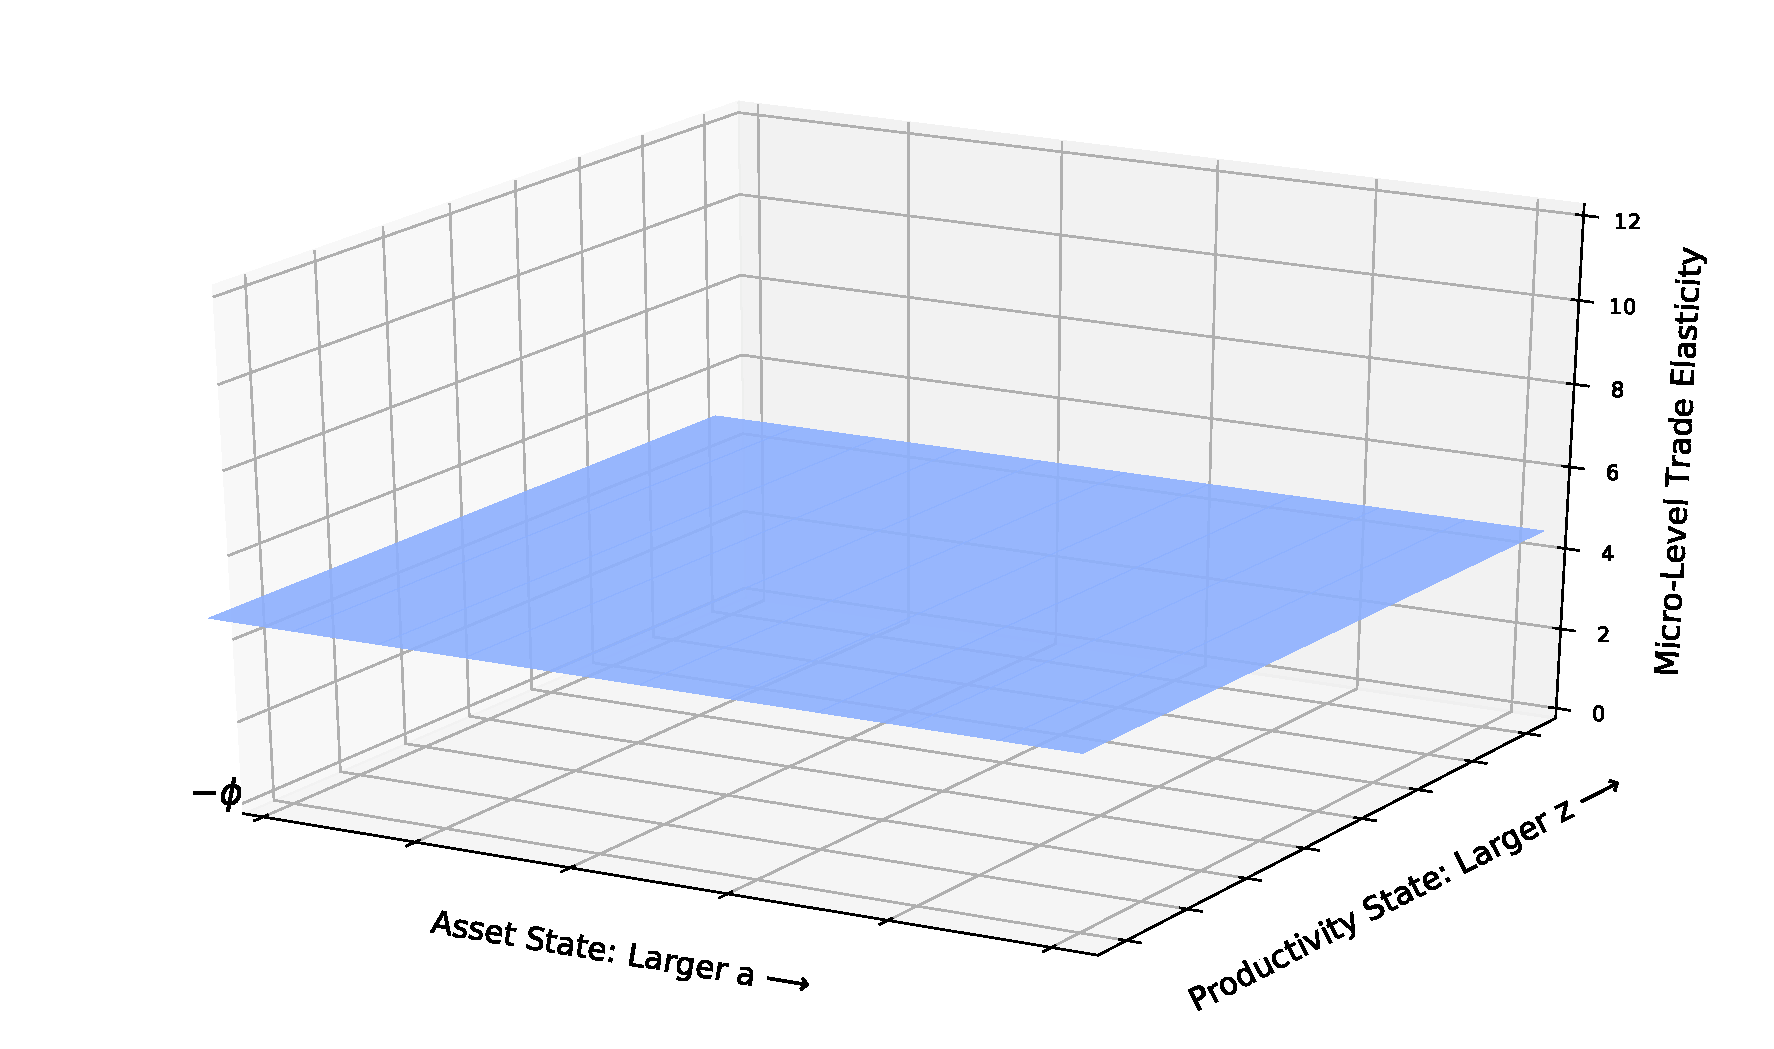
\includegraphics[scale = 0.57]{./figures/micro-elasticity-log.pdf}}
\caption{Log Preferences, Trade Elasticities, $-\theta_{ij}(a,z)$}\label{fig:log-elasticity}
\end{figure}


\begin{figure}[!t]
\centering{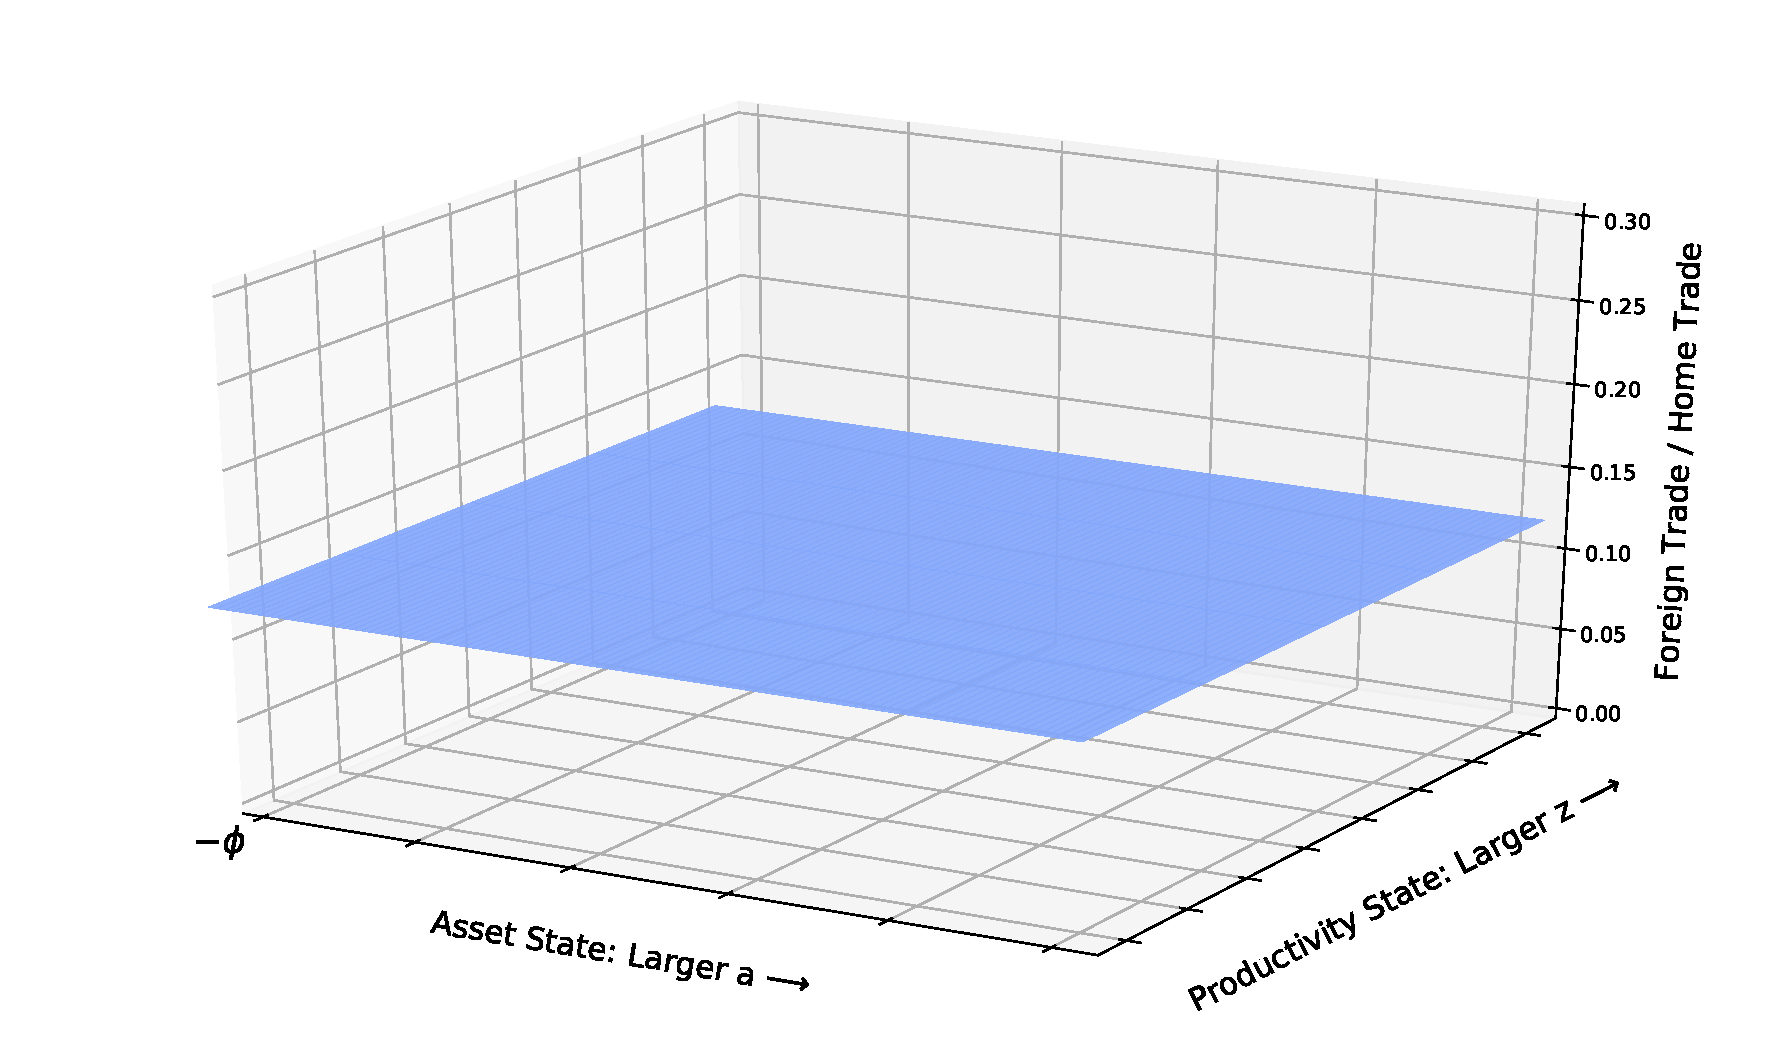
\includegraphics[scale = 0.57]{./figures/trade-share-log.pdf}}
\caption{Log Preferences, Trade, $M_{ij}(a,z) / M_{ii}(a,z)$ }\label{fig:log-micro-trade}
\end{figure}

}





\newpage


\section{Appendix: Endogenous Grid Method}

First, I'm going to derive the Euler equation for this model. I'll abstract from the situation in which the HH is at the borrowing constraint.

Focus on the within a variety choice component, the households value function can be written as:
\begin{align}
v_{ij}(a, z) = \max_{a'} u \left( \frac{R_i a + w_i z - a'}{p_{ij}} \right) + \beta  \mathrm{E} v(a', z')
\end{align}
then the first order condition associated with this problem is:
\begin{align}
\frac{u'(c_{ij}(a, z))}{p_{ij}} = \beta \mathrm{E} \frac{\partial v(a', z')}{\partial a'}
\end{align}
which is saying that, conditional on a variety choice the left hand side is the loss in consumption units which is $1 / p_{ij}$ evaluated at the marginal utility of consumption and then this is set equal to the marginal gain from saving a bit more which is how the value function changes with respect to asset holdings. Now we can arrive at the $\frac{\partial v(a', z')}{\partial a'}$ in the following way, so start from the log-sum expression for the expected value function
\begin{align}
\mathbb{E}_{\epsilon} v(a', z') =  \sigma_{\epsilon} \log \left\{ \sum_{j'} \exp \left( \frac{  v_{ij}(a', z')}{\sigma_{\epsilon}} \right) \right\}
\end{align}
and then differentiate this with respect to asset holdings which gives:
\begin{align}
\frac{\partial \mathbb{E}_{\epsilon} v(a', z')}{\partial a'} = \left( \frac{\sigma_{\epsilon}}{\sum_{j'} \exp \left( \frac{  v_{ij}(a', z')}{\sigma_{\epsilon}}\right)} \right)
\left[ \sum_{j'} \exp \left( \frac{  v_{ij}(a', z')}{\sigma_{\epsilon}}\right) \frac{1}{\sigma_{\epsilon}} \frac{\partial v_{ij}(a', z')}{\partial a'}  \right]
\end{align}
Then if you look at this carefully and notices how the choice probabilities from (\ref{eq:choice-prob}) are embedded in here, we have:
\begin{align}
\frac{\partial \mathbb{E}_{\epsilon} v(a', z')}{\partial a'} = \sum_{j'} \pi_{ij}(a', z) \frac{\partial v_{ij}(a', z')}{\partial a'}
\end{align}
and then we can just apply the Envelop theorem to the value functions associated with the discrete choices across the options:
\begin{align}
\frac{\partial \mathbb{E}_{\epsilon} v(a', z')}{\partial a'} = \sum_{j'} \pi_{ij}(a', z') \frac{u'(c_{ij}(a', z'))R_{i}}{p_{ij}}
\end{align}
So then putting everything together we have:
\begin{align}
\frac{u'(c_{ij}(a, z))}{p_{ij}} = \beta R_{i} \mathrm{E}_{z'} \left[ \sum_{j'} \pi_{ij}(a', z') \frac{u'(c_{ij}(a', z'))}{p_{ij}} \right]
\end{align}
where this has a very natural form: you set the marginal utility of consumption today equal to the marginal utility of consumption tomorrow adjusted by the return on delaying consumption, and the expected value of the marginal utility of consumption which reflects how the uncertainty over both ones' preference over different varieties and shocks to efficiency units. Taking into account the borrowing constraint then gives the generalized Euler equation from which the endogenous grid method will exploit:
\begin{align}
\frac{u'(c_{ij}(a, z))}{p_{ij}} = \max \left\{ \beta R_{i} \mathrm{E}_{z'} \left[ \sum_{j'} \pi_{ij}(a', z') \frac{u'(c_{ij}(a', z'))}{p_{ij}} \right] \ , \  u' \left( \frac{R_i a + w_i - \phi_{i}}{p_{ij}} \right) \right \}
\label{eq:apx-euler_equation}
\end{align}

\subsection{EGM-Discrete Choice Algorithm}

Here is a proposed approach. This focuses on just the consumer side in one country $i$.
\begin{itemize}
\item[\textbf{0.}] Set up an asset grid as usual. Then guess (i) a consumption function $g_{c,ij}(a,z)$ for each $a$, $z$, and product choice $j$ and (ii) choice specific value function $v_{ij}(a,z)$.

\item[\textbf{1.}] Compute the choice probabilities from (\ref{eq:choice-prob}) for each $(a,z)$ combination, given the guessed value functions.

\item[\textbf{1.}] Given the consumption function and choice probabilities compute the RHS of (\ref{eq:euler_equation}) first.

\item[\textbf{2.}] Then invert to find the new updated consumption choice so
\begin{align}
c_{ij}(\tilde a, z) = u^{' -1}\left\{ p_{ij} \max \left\{ \beta R_{i} \mathrm{E}_{z'} \left[ \sum_{j'} \pi_{ij}(a', z') \frac{u'(c_{ij}(a', z'))}{p_{ij}} \right] \ , \  u' \left( \frac{R_i a + w_i - \phi_{i}}{p_{ij}} \right) \right \} \right \}
\end{align}
where $u^{' -1}$ is the inverse function of the marginal utility of consumption.

Side note: One of the interesting things about this equation is that the direct $j$ component on the RHS that only affects the consumption choice is through the price. Can this be exploited? We also know the choice probabilities need to sum to one, so is there a way to map the consumption choice into the choice probabilities? Also, can interpolation be done once how $p$ scales things...

\item[\textbf{3.}] The key issue in this method is that we have found  $c_{ij}(\tilde a, z)$ where the consumption function is associated with some asset level that is not necessarily on the grid. The solution is to (i) use the budget constraint and infer $\tilde a$ given that $a'$ was chosen above (that's where we started), $z$, and $c_{ij}(\tilde a, z)$. Now we have a map from $\tilde a$ to $a'$ for which one can use interpolation to infer the $a'$ chosen given $a$ where $a$ is on the grid.

\item Do steps \textbf{2.} and \textbf{3.} for each $j$ variety choice. This then makes the function $g_{ij}(a,z)$ mapping each state and $j$ choice (today) into $a', z'$ states and then from the budget constraint we have an associated consumption function $g_{c,ij}(a,z)$

\item[\textbf{4.}] Compute the $\mathrm{E}\left[ v(g_{a,ij}(a,z), z') \right]$. This is performed in the {\tt{make\_Tv\_upwind!}} function. It fixes a country $j$, then works through shocks and asset states today and from the policy function $g_{a,ij}(a,z)$ figures out the asset choice tomorrow. Then the $\mathrm{E}\left[ v(g_{a,ij}(a,z), z') \right]$ is (\ref{eq:log_sum}) over the different variety choices tomorrow (this is the integration over $\epsilon$) multiplied by the probability of $z'$ occurring (this is the integration over $z$).

\item[\textbf{5.}] Given \textbf{4.} update the value function using the bellman equation evaluated at the optimal policies:
\begin{align}
Tv_{ij}(a, z) = u(g_{c,ij}(a,z)) + \beta \mathrm{E}\left[ v(g_{a,ij}(a,z), z') \right]
\end{align}

\item[\textbf{6.}] Compare old and new policy functions, old and new value functions, and then update accordingly.


%\item[\textbf{5.}] Given the structure of $Q$, then just line (\ref{eq:utility_azj}) with $Q$ and invert to find value functions that are associated with each $(a,z,j)$ state. This takes the form where
%\begin{align}
%\vec{v} = (\mathbb{I} - \beta Q) \ / \  \vec{u} \label{eq:v_inversion}
%\end{align}
%where, again, each entry in $\vec{u}$ is an $(a,z,j)$ state and it conforms with the analogues entries in $Q$ of the $(a,z,j)$ states and then the resulting output $\vec{v}$ are the value functions corresponding with $(a,z,j)$ state.
%
%\item[\textbf{6.}] Given $v_{ij}(a,z)$ computed from (\ref{eq:v_inversion}), now compute choice probabilities using (\ref{eq:choice-prob}) for each $(a,z)$ combination.
\end{itemize}



\newpage

\bibliography{./bibtex/micro_price_bibtex}

\end{onehalfspacing}

\end{document} 